\documentclass[12pt]{niuthesis}

% line numbers for draft
\usepackage{lineno}
\linenumbers{}

\usepackage{latexsym}
\usepackage{graphicx}
\usepackage{xspace}
\usepackage{amssymb}
\usepackage{amsmath}
\usepackage{rotating}
\usepackage{multirow}
\usepackage{longtable}
\usepackage{booktabs}
\usepackage[tableposition=top]{caption}

\usepackage[
  style=numeric-comp,
  sorting=none,
  giveninits=true
]{biblatex}
\renewbibmacro{in:}{}
\bibliography{main}

\usepackage{hyperref}
\hypersetup{
  bookmarksnumbered,%
  bookmarksopen,%
  bookmarksopenlevel=1,%
  colorlinks=false,%
  pdfborder={0 0 0},%
  plainpages=false,%
  pdfencoding=auto,%
  psdextra,%
  linktoc=all,%
  pdfauthor={},%
  pdftitle={},%
  pdfsubject={},%
  pdfkeywords={your topics}%
}

\usepackage[
  nopostdot,toc,acronym,
  nomain,nonumberlist,nogroupskip
]{glossaries}
\glsdisablehyper{}

\usepackage{epigraph}

\setlength\epigraphwidth{0.9\textwidth}
\setlength\epigraphrule{0pt}

\makeatletter
\AtBeginDocument{%
  \let\thMakeUppercase\uppercase%
}
\makeatother

% Load glossary and set style
%\makeglossaries{}
%\newglossarystyle{mylong}{
%  \setglossarystyle{long}
%  \renewenvironment{theglossary}%
%  {\setlength\LTleft{0pt}
%   \setlength\LTright{0pt}
%   \setlength{\glsdescwidth}{0.85\linewidth}
%   \begin{longtable}{@{}lp{\glsdescwidth}@{}}}%
%  {\end{longtable}}
%  \renewcommand*{\glsgroupskip}{}
%}
%\setglossarystyle{mylong}
%\setacronymstyle{long-short}

\loadglsentries{glossary}

% List of Symbols
%\newcommand{\listofXXX}{% List of Acronyms
\glsaddall{}
\printglossary[
  title=List of Acronyms,
  type=\acronymtype,
]

% \chapter*{List of Blah}
% \addcontentsline{toc}{chapter}{List of Blah}}

\begin{document}

% Load macros and definitions
\newcommand{\twochoices}[2]{
    \left \{%
    \begin{array}{lcc}
        \displaystyle #1 \\
        \vspace{-10pt}   \\
        \displaystyle #2
    \end{array}
    \right.
}

\newcommand{\twovec}[2]{
    \left(%
    \begin{array}{c}
        #1 \\ #2
    \end{array}
    \right)
}

\newcommand{\twomatrix}[4]{
    \left(%
    \begin{array}{cc}
        #1 & #2 \\
        #3 & #4
    \end{array}
    \right)
}
\newcommand{\FASTJET}{\textsc{Fastjet}\xspace}

\newcommand{\MADGRAPH}{\textsc{MadGraph}\xspace}
\newcommand{\MCATNLO}{\textsc{mc@nlo}\xspace}
\newcommand{\MGvATNLO}{\MADGRAPH{}5\_a\MCATNLO}
\newcommand{\POWHEG}{{\textsc{powheg}}\xspace}
\newcommand{\GEANTfour}{{\textsc{Geant4}}\xspace}
\newcommand{\PYTHIA}{{\textsc{pythia}}\xspace}
\newcommand{\NanoAOD}{{\textsc{NanoAOD}}\xspace}
\newcommand{\ROOT}{{\textsc{ROOT}}\xspace}

\newcommand{\Wplusminus}{W\ensuremath{^{\pm}}}
\newcommand{\Wplus}{W\ensuremath{^{+}}}
\newcommand{\Wminus}{W\ensuremath{^{-}}}

\newcommand{\de}{\ensuremath{^\circ}}
\newcommand{\ten}[1]{\ensuremath{\times \text{10}^\text{#1}}}
\newcommand{\unit}[1]{\ensuremath{\text{\,#1}}\xspace}
\newcommand{\mum}{\ensuremath{\,\mu\text{m}}\xspace}
\newcommand{\micron}{\ensuremath{\,\mu\text{m}}\xspace}
\newcommand{\km}{\ensuremath{\,\text{km}}\xspace}
\newcommand{\m}{\ensuremath{\,\text{m}}\xspace}
\newcommand{\cm}{\ensuremath{\,\text{cm}}\xspace}
\newcommand{\mm}{\ensuremath{\,\text{mm}}\xspace}
\newcommand{\mus}{\ensuremath{\,\mu\text{s}}\xspace}

\newcommand{\seconds}{\ensuremath{\,\text{s}}\xspace}
\newcommand{\nanoseconds}{\ensuremath{\,\text{ns}}\xspace}

\newcommand{\Tesla}{\ensuremath{\,\text{T}}\xspace}

\newcommand{\sqrtOfs}{\ensuremath{\,\sqrt{s}}\xspace}

\newcommand{\keV}{\ensuremath{\,\text{ke\hspace{-.08em}V}}\xspace}
\newcommand{\MeV}{\ensuremath{\,\text{Me\hspace{-.08em}V}}\xspace}
\newcommand{\GeV}{\ensuremath{\,\text{Ge\hspace{-.08em}V}}\xspace}
\newcommand{\TeV}{\ensuremath{\,\text{Te\hspace{-.08em}V}}\xspace}

\newcommand{\fbinv}{\mbox{\ensuremath{\,\text{fb}^{-1}}}\xspace}
\newcommand{\pbinv}{\mbox{\ensuremath{\,\text{pb}^{-1}}}\xspace}

\newcommand{\lumi}{\ensuremath{\mathcal{L}}\xspace}

\newcommand{\LLow}{\ensuremath{\mathcal{L}=\text{10}^\text{33}\,\text{cm}^\text{\(-\)2}\,\text{s}^\text{\(-\)1}}\xspace}
\newcommand{\LMed}{\ensuremath{\mathcal{L}=\text{2}\times \text{10}^\text{33}\,\text{cm}^\text{\(-\)2}\,\text{s}^\text{\(-\)1}}\xspace}
\newcommand{\LHigh}{\ensuremath{\mathcal{L}=\text{10}^\text{34}\,\text{cm}^\text{\(-\)2}\,\text{s}^\text{\(-\)1}}\xspace}

\newcommand{\pt}{\ensuremath{p_{\mathrm{T}}}\xspace}
\newcommand{\ET}{\ensuremath{E_{\mathrm{T}}}\xspace}
\newcommand{\HT}{\ensuremath{H_{\mathrm{T}}}\xspace}
\newcommand{\mT}{\ensuremath{m_{\mathrm{T}}}\xspace}

\newcommand{\CL}{\ensuremath{\text{CL}}\xspace}
\newcommand{\CLs}{\ensuremath{\text{CL}_\text{s}}\xspace}
\newcommand{\CLsb}{\ensuremath{\text{CL}_\text{s+b}}\xspace}


\title{Studies of vector boson scattering in the semileptonic \textit{ZV} channel with the CMS detector at \( \sqrt{\MakeLowercase{s}} \) = 13 TeV}

\author{Ramanpreet Singh}

\major{Physics}
\degree{Dissertation}{Ph.D.}{Doctor of Philosophy}
\degreedate{Summer}{2022}
\department{Department of Physics}
\director{Vishnu Zutshi}

\begin{abstract}
  This dissertation reports on the search for
the \gls{VBS} in semileptonic channel \textit{ZV},
where the \textit{Z} boson decays to a pair of leptons (electrons or muons),
and the other vector boson \textit{V} (either \textit{W} or \textit{Z})
decays hadronically to a pair of jets, in association of two jets
i.e.~\( \textit{ZV}jj \rightarrow l^{+}l^-jjjj \), \( l=e \) or \( \mu \).
The search used 137 \fbinv{} of proton-proton collision data collected by
the \gls{CMS} experiment at the \gls{LHC} with
center-of-mass energy (\( \sqrt{s} \)) of 13 \TeV{} from 2016 to 2018.
\gls{VBS} is a key process in understanding the nature of \gls{EWSB} in
the framework of \gls{SM}.

Studies and instrumentation done towards the future detector
upgrade to the \gls{CMS} experiment which will replace
the current endcap \gls{HCAL} and \gls{ECAL} with \gls{HGCAL}
during \gls{LS3} are also reported.
Optimal configuration
of scintillator tiles coupled to \glspl{SiPM}
in the \gls{HGCAL} is measured and suggested using testbeam measurement of
scintillator tiles and noise measurement of \glspl{SiPM}.
Prototyping of automated wrapping of scintillator tiles in \gls{ESR} film
are also discussed.

\end{abstract}

\begin{acknowledgments}
  First, I would like to thank my advisor, Vishnu Zutshi
for giving me opportunities to make this work possible.
Your mentorship and guidance over the last six years has
contributed to my growth as a scientist and as a person. Thank you
for all the discussions and being patient with me.
I would also like to thank my committee members Michael (Mike) Eads,
Gerald (Jerry) Blazey, and Jeffrey Berryhill for providing feedback
on my dissertation.

For the analysis, I would like to thank Michael (Mike) Eads, for providing
guidance and suggestions throughout the analysis.
I would also like thank Jeffrey Berryhill, Aram Apyan, Jay Lawhorn
and CMS collaboration for their help and guidance.


I would like to thank Alexandre (Sasha) Dychkant for
teaching me various lab equipments and sharing his experimental knowledge.
I would also like to thank
Iman Salehinia, Nicholas Pohlman, Michael Figora, Todd Fletcher,
and Brian Scott who made the instrumentation of
scintillator tile wrapping machine possible.

I would like to thank NIU physics faculty and staff. I would also
like to thank my fellow graduate students
Prudhvi Raj Varma Chintalapati,
Christina Sarosiek,
Brendan Leung,
Aakaash Narayanan,
Osama Mohsen,
Ben Simons,
Wei Hou Tan,
Austin Dick,
Andrew Best,
Prudhvi Nikhil Bhattiprolu,
Will Baker,
Kevin Hamilton,
Jeremiah Mitchell,
and Sebastian Szustkowski
for being great friends.


Lastly, I would like to thank my family for their constant
support and love throughout my time away from home.
\end{acknowledgments}

\begin{dedication}
  I dedicate this dissertation to my mother, \textit{Harsharan Kaur};
my father, \textit{Lakhmir Singh};
and my brother; \textit{Gurpreet Singh} for their love and support.
\end{dedication}

% Make Prologue
\MakeThesisPrologue{}

% Reset glossary acronyms
\glsresetall{}

% Chapters
\chapter{
  Introduction
 }\label{ch_intro}

\epigraph{\textit{It doesn't matter how beautiful your theory is,
    it doesn't matter how smart you are. \\
    If it doesn't agree with experiment, it's wrong.
    In that simple statement is the key to science.}}
{--- Richard P. Feynman}

``Particle Physics'' is the branch of physics which deals with the fundamental
particles and the interactions between them. Fundamental particles are the
subatomic particles which are not made of other particles.
There are two types of fundamental particles ``matter'' and ``interaction''
particles, as the name suggests matter particles are the fundamental constituent of matter and
the interactions between among them is governed by how they exchange interaction particles.
\gls{SM} of particle physics is the theory that classifies these fundamental
particles and describes three out of four fundamental
interaction forces; electromagnetic, weak, and strong.

This chapter introduces briefly to the theory of \gls{SM}, Higgs mechanism,
spontaneous \gls{EWSB}, \gls{VBS}, and the motivation for the search of \gls{VBS}
in semileptonic decay channel ZV with leptonic decay of Z,
and hadronic decay of V (W/Z) to pair of quarks.

\section{
  Standard model
 }\label{ch_intro:standard-model}

In \gls{SM}, the matter particles are fermions, and
the interaction particles are bosons. \gls{SM} also includes
anti-fermions, which are fermions with equal mass but opposite sign of charge.
Figure~\ref{fig:standard-model-details} lists mass, electric charge,
and spin of fermions and bosons in \gls{SM}.

Fermions obey Fermi-Dirac statistics and have half integer spin. They can be further
divided into leptons which have integral electric charge, and quarks which have
fractional electric charge. There are three generations of quarks and leptons
discovered to the date, each generation only differs by the mass.
In addition to the electric charge, quarks also have
three types of ``color'' charge (red, green and blue). Quarks cannot be isolated
because of ``color confinement'', which requires net color charge to be zero
for an isolated particle, for this reason we can only have certain composition
of quarks. Baryons (proton, neutrons, etc.) are made up of three quarks with
each with different color charge,
and mesons (pions, kaons, etc.) are made of two quarks with color and anti-color charge.

Bosons obey Bose-Einstein statistics and have integral spin.
They are described by local gauge theory and are also called gauge boson.
Photons are the interaction particle of electromagnetic force, they are massless
and only interact with charged particles. Gluons are the mediator of strong force
between quarks, they are massless and carries color charge. \Wplusminus{} and Z
are the vector bosons and mediator of weak force,
unlike photons and gluons they are massive. \Wplus{} and \Wminus{}
are antiparticles of each other, and Z is antiparticle of its own.
The last gauge boson Higgs is a massive scalar boson with zero spin,
zero electric and color charge. Higgs boson is not a force carrier,
but rather explains why only some particles have mass.

The \gls{SM} is built in the framework of \gls{QFT}, in which particles
are excitation of the fields and interactions arise from local gauge
invariance. The \gls{SM} is a \( {SU(3)}_C \otimes {SU(2)}_L \otimes {U(1)}_Y\)
gauge theory, \( {U(1)}_Y \), \( {SU(2)}_L \), \( {SU(3)}_C \) are the gauge symmetries
of \gls{QED}, weak interaction and \gls{QCD} respectively, where the indices
stands for ``hypercharge'' (Y), ``left-handed'' (L) and ``color'' (C).

\begin{figure}[!ht]
  \centering
  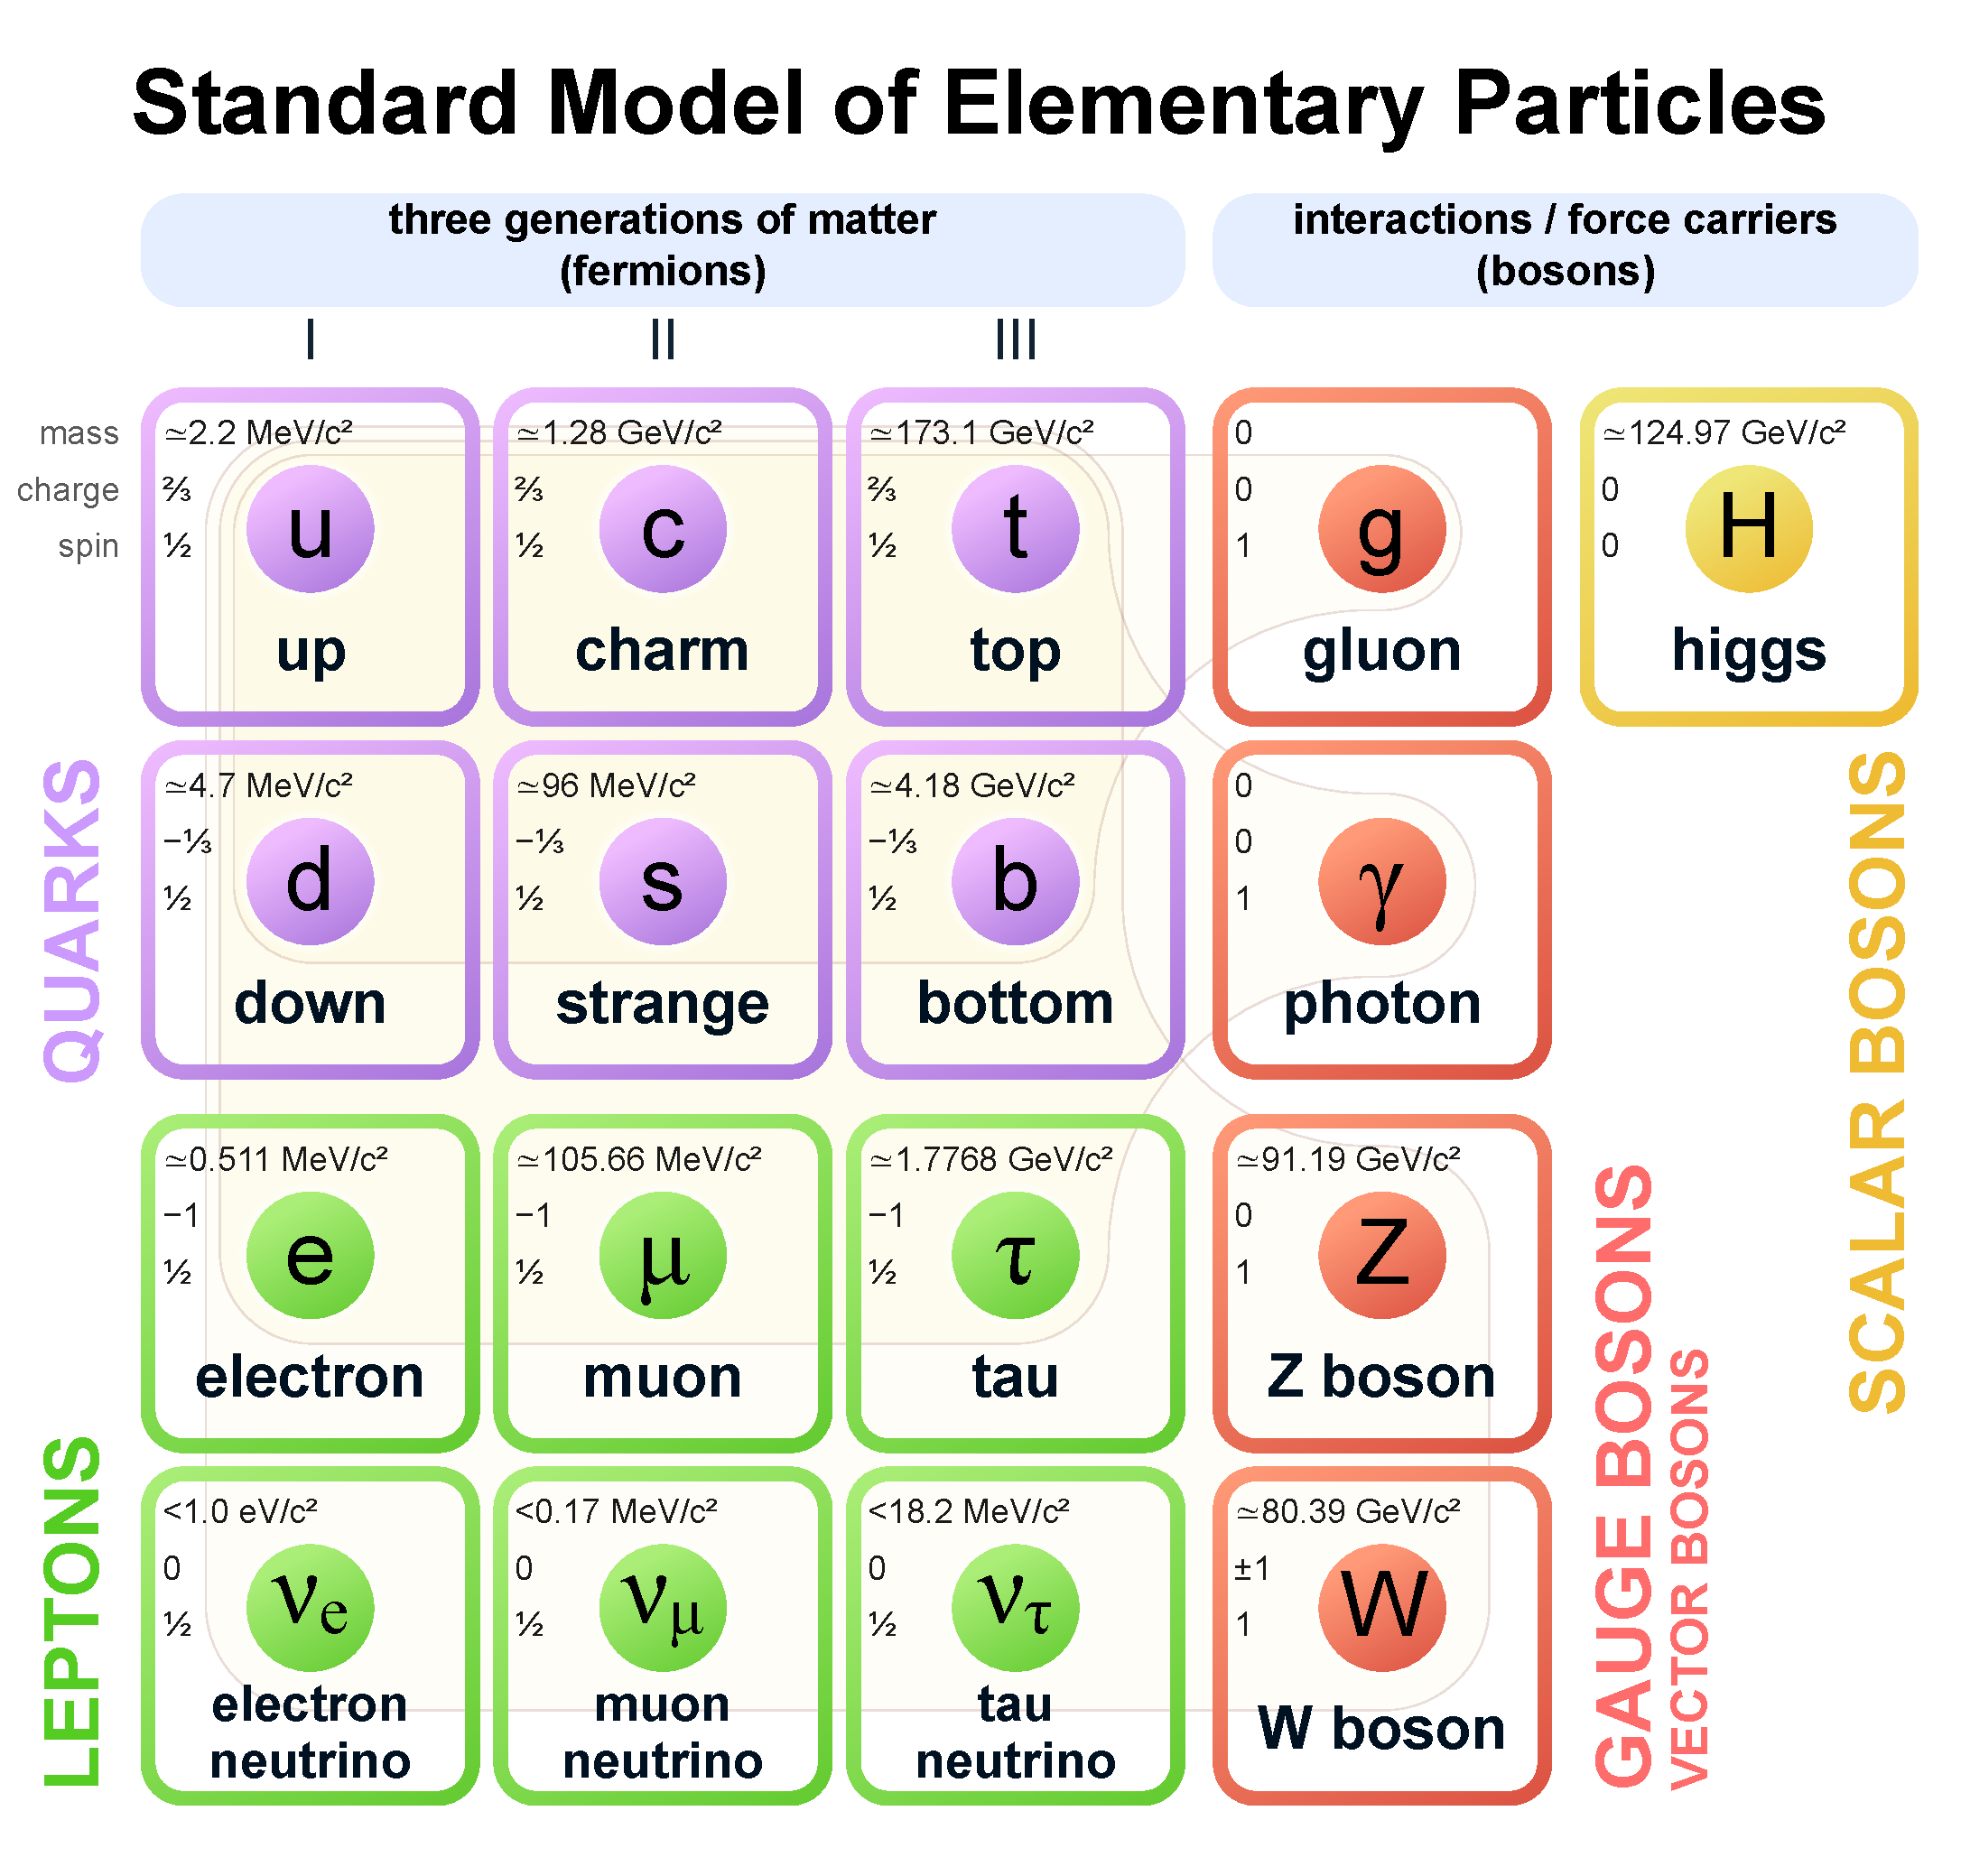
\includegraphics[width=0.8\textwidth]{figures/Standard_Model_of_Elementary_Particles.pdf}
  \caption[Standard model list of matter and interaction particles]%
  {Standard model list of matter and interaction particles~\cite{image-standard-model}}%
  \label{fig:standard-model-details}
\end{figure}

\subsection{
  Quantum Electrodynamics (QED)
}\label{ch_intro:qed}

\gls{QED} is a quantum field theory of electrodynamics, it describes
the interaction of photons to the charged fermions.
The \gls{QED} is local gauge invariant and symmetric with \( {U(1)}_{Q} \) group,
defined as,
%
\begin{align}
  {U(1)}_{Q} = \exp\left( { i Q \theta (x) } \right)
\end{align}

where \( \theta (x) \) is any spacetime function also called gauge parameter,
and \( Q \) is coupling constant of photon field to the fermions
which is equivalent to the charge of fermion.

Under this transformation, fermion spinor \( \psi (x) \) and
four-potential \( A_{\mu} \) electromagnetic tensor will transform
as,
%
\begin{align}
  \psi (x) \rightarrow {U(1)}_{Q} \psi (x) \\
  A_{\mu} \rightarrow A_{\mu} - \frac{1}{e} \partial_{\mu} \theta
\end{align}

The general Lagrangian of \gls{QED} for fermions and their interaction
with photon field is given by,
%
\begin{equation}\label{eq:lag-qed}
  {\mathcal{L}}_{QED} = \bar{\psi} ( i {\gamma}^{\mu} {D}_{\mu} - m ) \psi
  - \frac{1}{4} {F}_{\mu \nu} {F}^{\mu \nu}
\end{equation}

where \( m \) is the mass of fermion,
\( {D}_{\mu} \) is the covariant derivative,
and \( {F}_{\mu \nu} \) is the electromagnetic field tensor defined as,
%
\begin{align}
  {D}_{\mu} = \partial_{\mu} + i Q A_{\mu} \\
  {F}_{\mu \nu} = \partial_{\mu} A_{\nu} - \partial_{\nu} A_{\mu}
\end{align}

\subsection{
  Quantum Chromodynamics (QCD)
}\label{ch_intro:qcd}

The strong interactions are represented by \( {SU(3)}_{C} \) gauge group, invariant
under transformations of color charge degree of freedom, and it is based
on Yang-Mills theory~\cite{Yang-Mill:1954}. Since ``electrodynamics''
is the theory of electric charge, this theory of color (\textit{chromo} in Greek)
charge is called ``chromodynamics'', hence the name \glsfirst{QCD}.

A quark spinor in initial state can be represented as,
%
\begin{equation}
  \psi = \left( \begin{matrix}
    \psi_{red}  \\
    \psi_{blue} \\
    \psi_{green}
  \end{matrix} \right)
  = \left( \begin{matrix}
    \psi_{1} \\
    \psi_{2} \\
    \psi_{3}
  \end{matrix} \right)
\end{equation}

\( {SU(3)}_{C} \) is an exact symmetry, it means the difference between
colors cannot be measured experimentally, thus the color labels in quark spinor are arbitrary.
\( {SU(3)}_{C} \) transformation is defined as,
%
\begin{equation}
  {SU(3)}_{C} = \exp \left( {i \theta^{a}(x) \frac{\lambda^{a}}{2}} \right)
\end{equation}

where \( \lambda^{a} \) for \( a = 1,\ldots,8\),
are the Gell-Mann matrices, and \( \theta^{a}(x) \) are any gauge parameters.
These eight generators of symmetry corresponds to eight gauge vector boson gluons.

Similar to \gls{QED}, the covariant derivative for \gls{QCD} can be formed as,
%
\begin{equation}
  D_{\mu} = \partial_{\mu} + i g_s \frac{\lambda^{a}}{2} G_{\mu}^{a}
\end{equation}

where \( g_s \) is the coupling constant of gluon to the quarks,
and \( G_{\mu}^{a} \) are the eight gauge fields corresponding to gluons.

Now the corresponding field strength tensor in \gls{QCD} can be formed as,
%
\begin{equation}
  F_{\mu \nu}^{a} = \partial_{\mu} G_{\nu}^{a} - \partial_{\nu} G_{\mu}^{a}
  - g_s f^{abc} G_{\mu}^{b} G_{\nu}^{c}
\end{equation}

where \( f^{abc} \) are the structure constants of \( {SU(3)}_{C} \)
which satisfy \( [\lambda^{a}, \lambda^{b}] = i f^{abc} \lambda^{c} \) relation.

The full Lagrangian for \gls{QCD} can now be constructed as,
%
\begin{equation}
  {\mathcal{L}}_{QCD} = {\bar{\psi}}^{i}
  ( i {\gamma}^{\mu} {{D}_{\mu}}^{ij} - m \delta^{ij} )\psi^{j}
  - \frac{1}{4} {F}_{\mu \nu}^{a} {F}^{a \mu \nu}
\end{equation}

for mass \( m \), indices \( i \) and \( j \) runs from 1 to 3.

The main difference of gluon field with respect to photon field is
the presence of third term in
field strength tensor which allows triplet and quartic
self coupling of gluons.

\subsection{
  Electroweak Theory
}\label{ch_intro:ew}

The theory of weak interaction which changes the flavor of fermions is
called \gls{QFD}. Since the unification of electromagnetic
and weak interaction into \gls{EW} interaction by
Glashow, Weinberg, and Salam~\cite{Glashow1959,Weinberg1967,Salam1959},
the weak interaction is better understood in terms of \gls{EW} theory.

Weak interaction only couples to left-handed fermions and it is same
whether the fermion is charged or not. The underlying gauge group of
\gls{EW} interaction is \( {SU(2)}_{L} \otimes {U(1)}_{Y} \) and
has two transformations one for the left-handed doublet
\( L \) and the right handed singlet fermions \( \psi_R \) which are defined as,
%
\begin{align}
  {SU(2)}_{L} \otimes {U(1)}_{Y} & =
  \exp \left( {i \theta^{a}(x) \frac{\sigma^a}{2}} + {i \theta(x) \frac{Y}{2}} \right)
  , \quad (doublet)                                                                \\
                                 & = \exp \left( {i \theta(x) \frac{Y}{2}} \right)
  , \quad (singlet)
\end{align}

where \( Y \) is the hypercharge (linear combination of electric charge and weak
isospin component), and \( \sigma^{a} \) for \( a = 1,2,3 \)
are the Pauli spin matrices generator of \( SU(2) \) symmetry. Left-handed
fermion \( L \) doublets are,
%
\begin{equation}
  L = \left(\begin{matrix}
    \nu_e \\
    e_L
  \end{matrix}\right) ,
  \left(\begin{matrix}
    \nu_\mu \\
    \mu_L
  \end{matrix}\right) ,
  \left(\begin{matrix}
    \nu_\tau \\
    \tau_L
  \end{matrix}\right) ,
  \left(\begin{matrix}
    u_L \\
    d_L
  \end{matrix}\right) ,
  \left(\begin{matrix}
    c_L \\
    s_L
  \end{matrix}\right) ,
  \left(\begin{matrix}
    t_L \\
    b_L
  \end{matrix}\right)
\end{equation}

and right-handed singlets are,
%
\begin{equation}
  \psi_R = e_R, \mu_R, \tau_R, u_R, d_R, c_R, s_R, t_R, b_R
\end{equation}

The covariant
derivative of \gls{EW} is then,
%
\begin{align} \label{eq:ew-dmu}
  D_{\mu} L      & = \left( \partial_{\mu} + i g_w \frac{\sigma^{a}}{2} W^{a}_{\mu} + i g \frac{Y}{2} B_{\mu} \right) L \\
  D_{\mu} \psi_R & = \left( \partial_{\mu} + i g \frac{Y}{2} B_{\mu} \right) \psi_R
\end{align}

where \( W^{a}_{\mu} \) and \( B_{\mu} \) are the gauge fields. The \gls{EW}
Lagrangian can now written as,
%
\begin{align}
  \mathcal{L}_{EW} = i \bar{L} \gamma^{\mu} D_{\mu} L
  + i \bar{\psi}_R \gamma^{\mu} D_{\mu} \psi_R
  - \frac{1}{4} {W}_{\mu \nu}^{a} {W}^{a \mu \nu}
  - \frac{1}{4} {B}_{\mu \nu} {B}^{\mu \nu}
\end{align}

where \( B_{\mu \nu} \) and \( W^{a}_{\mu \nu} \) are fields strength,
defined as,
%
\begin{align}
  B_{\mu \nu }    & = \partial_{\mu} B_{\nu} - \partial_{\nu} B_{\mu}         \\
  W_{\mu \nu}^{a} & = \partial_{\mu} W_{\nu}^{a} - \partial_{\nu} W_{\mu}^{a}
  - g_w \epsilon^{abc} W_{\mu}^{b} W_{\nu}^{c}
\end{align}

the linear combination of \( B_{\mu} \) and \( W_{\mu} \) gauge field, with a weak mixing
angle \( \theta_w \) gives 4 vectors boson \Wplus, \Wminus, Z, and \( \gamma \) of \gls{SM},
%
\begin{align}
  W^{\pm}_{\mu} & = \frac{1}{\sqrt{2}} \left( W^{1}_{\mu} \mp W^{2}_{\mu} \right) \\
  Z_{\mu}       & = \cos \theta_w W^{3}_{\mu} - \sin \theta_w B_{\mu}             \\
  A_{\mu}       & = \sin \theta_w W^{3}_{\mu} + \cos \theta_w B_{\mu}             \\
  \tan \theta_w & = g/g_{w}
\end{align}

Similar to \gls{QCD}, the presence of third term in field strength tensor
allows the self triple (WWZ, WW\( \gamma \)) and quartic (WWWW, WWZZ,
WWZ\( \gamma \), WW\( \gamma \gamma \)) couplings.

\subsection{
  Electroweak Symmetry Breaking and Higgs Mechanism
}\label{ch_intro:ewsb}

The \textit{spontaneous symmetry breaking} is the phenomena which explains
why the ground state is not invariant under the symmetry
of the Lagrangian. The ``spontaneous'' means the symmetry
breaking is not done by external agent but rather by Lagrangian itself
in ground state.

The \gls{EW} theory unifies weak interaction and \gls{QED} but the
gauge boson in \gls{EW} theory are all massless, if we were to add mass
terms like \( - m^{2} W_{\mu} W^{\mu} \) by hand, it will no longer
be gauge invariant. The solution to this without breaking gauge invariance
is spontaneous symmetry breaking, but this requires addition of new scalar
field called Higgs field via \gls{BEH}~\cite{Englert1964,Higgs1964}, and this
symmetry breaking is known as \glsfirst{EWSB}.

\gls{BEH} introduces a complex scalar field as \( {SU(2)}_L \)
doublet with non-zero \gls{VEV},
%
\begin{equation}
  \phi = \left( \begin{matrix}
      \phi^{+} \\
      \phi^{0}
    \end{matrix} \right)
  = \frac{1}{\sqrt{2}}
  \left( \begin{matrix}
      \phi^{1} + i \phi^{2} \\
      \phi^{3} + i \phi^{3}
    \end{matrix} \right)
\end{equation}

and \gls{BEH} Lagrangian is,
%
\begin{equation}
  \mathcal{L}_{BEH} = {| D_{\mu} \phi |}^{2} - V(\phi)
\end{equation}

where \( D_{\mu} \) is same as \gls{EW} covariant derivate
in Equation~\ref{eq:ew-dmu}, and \( V(\phi) \) is,
%
\begin{equation}
  V(\phi) = \mu^{2} |\phi|^{2} + {\lambda (|\phi|^{2})}^{2}
\end{equation}

the parameter \( \lambda \) is required to be positive,
for \( \mu^2 > 0\) the minima is at 0, which is not an interesting case,
but for \( \mu^2 < 0\) vacuum state energy is given by,
%
\begin{equation}
  \phi^{\dagger} \phi = - \frac{\mu^{2}}{2 \lambda}
\end{equation}

by the choice of non-zero \gls{VEV} \( v \), scalar field can be parameterized as,
%
\begin{align}
  v        & = \sqrt{\frac{- \mu^2}{\lambda}}                 \\
  \phi (x) & = \frac{1}{\sqrt{2}} \left( \begin{matrix}
                                             0 \\
                                             h (x) + v
                                           \end{matrix} \right)
\end{align}

where \( h(x) \) is the Higgs field and \gls{BEH} spontaneously breaks electroweak symmetry,
%
\begin{equation}
  {SU(2)}_L \otimes {U(1)}_Y \rightarrow {U(1)}_{EM}
\end{equation}

Visually the Higgs potential is shown in Figure~\ref{fig:higgs-potential}. The ball position
at the center represents unbroken symmetry, and at the minima represents spontaneous
broken symmetry in the ground state of potential.
%
\begin{figure}[!ht]
  \centering
  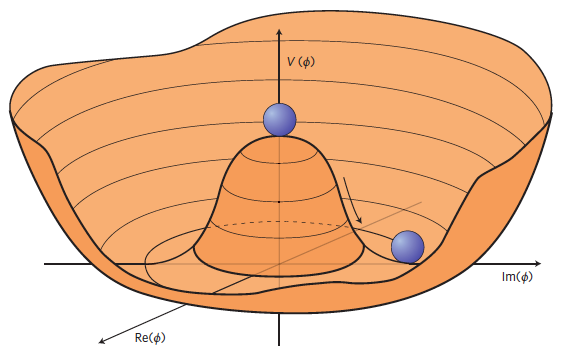
\includegraphics[width=0.7\textwidth]{figures/higgspotential.png}
  \caption[3D representation of Higgs potential]%
  {3D representation Higgs potential~\cite{image-higgs-potential}.}%
  \label{fig:higgs-potential}
\end{figure}

After \gls{EWSB}, the \gls{BEH} Lagrangian contains the following mass terms,
%
\begin{align}
  m^{2}_{W} W^{+}_{\mu} W^{- \mu}, \quad
  m^{2}{Z} Z_{\mu}Z^{\mu}, \quad m^{2} h^{2}
\end{align}

and gauge fields,
%
\begin{align}
  - \frac{1}{4} A_{\mu \nu} A^{\mu \nu}, \quad
  - \frac{1}{4} W^{+}_{\mu \nu} W^{- \mu \nu}, \quad
  - \frac{1}{4} Z_{\mu \nu} Z^{\mu \nu}, \quad
  - \frac{1}{4} {(\partial_{\mu} h)} {(\partial^{\mu} h)}
\end{align}

thus explaining existence of three massive vector boson (\Wplusminus{}, Z), one massless
vector boson (\( \gamma \)), and one massive scalar boson Higgs (H).

With experimentally measured value of \gls{VEV} \( v \) approximately 246 \GeV{},
The masses of bosons can be written in terms of \( v \) as,
%
\begin{align}
  m_A = 0, \quad
  m_W = \frac{g_{W} v}{2}, \quad
  m_Z = \frac{\sqrt{g^{2}_{W} + g^{2}} v }{2}, \quad
  m_H = \sqrt{2\lambda} v
\end{align}

\section{
  Vector Boson Scattering
 }\label{ch_intro:vbs}

The \glsfirst{VBS} is,
%
\begin{equation}
  VV \rightarrow VV
\end{equation}

that is, when you have two vector bosons in initial state and two vector
bosons in final state.

This section describes the motivation behind studying \gls{VBS}, and
the topology of scattering studied in this dissertation.

\subsection{Motivation}

A massless spin-1 boson can exists in two transverse polarization as,
%
\begin{equation}
  \varepsilon^{\mu}_{\pm} = \mp \frac{1}{\sqrt{2}} (0, 1, \pm i, 0)
\end{equation}

and massive vector bosons can also exists in one longitudinal polarization,
%
\begin{equation}
  \varepsilon^{\mu}_{L} = \frac{1}{m} (p_z, 0, 0 , E)
\end{equation}

This means the longitudinal polarized \gls{VBS} will scale as \( E/m \),
whereas the scattering of transverse polarized boson remains constant.
The Figure~\ref{fig:vbs-at-high-energies} shows the cross-section
of longitudinal polarized \gls{VBS} \( V_L V_L \to V_L V_L\)
for low to high energies. Perturbatively the cross-section of
longitudinal polarized \gls{VBS} will scale with center of mass energy
\( \sqrt{s} \) and eventually the unitarity is violated at
\( \approx 1.2 \TeV{} \) scale~\cite{Lee1977,Lee1977a}.
The Figure~\ref{fig:vbs-at-high-energies} also shows
how the existence of light Higgs boson and
inclusion of Higgs to vector boson coupling diagrams in longitudinal
polarized \gls{VBS} can restore unitarity violation, and
since the discovery of Higgs boson \( m_H = 125 \GeV{} \) in July 2012, the
\gls{VBS} studies became important and complementary to direct measurement of Higgs coupling
in \gls{SM}, and test for \gls{EWSB} at \TeV{} scale.

\begin{figure}[!ht]
  \centering
  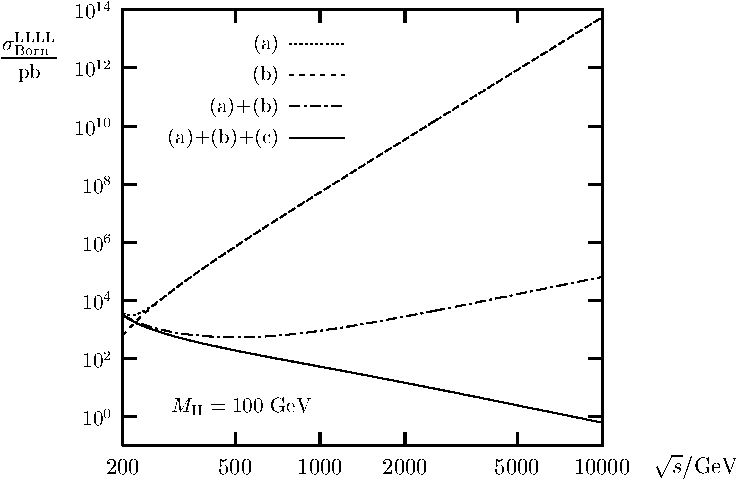
\includegraphics[width=0.7\textwidth]{figures/unitarity.pdf}
  \caption[The cross-sections for longitudinal polarized \gls{VBS} involving three
    and four-boson coupling with and without Higgs coupling included.]%
  {The cross-sections for longitudinal polarized \gls{VBS} involving three
    and four-boson coupling with and without Higgs coupling diagram included.
    (a) is for the diagrams with three-boson coupling,
    (b) is for diagrams with four-boson coupling, and (c) is for diagrams
    with Higgs to vector boson coupling.~\cite{Denner1997}}%
  \label{fig:vbs-at-high-energies}
\end{figure}

\subsection{
  Topology of VBS in Semileptonic ZV Final State
}

In proton-proton collisions, the actual interaction happens
with the constituent quarks. For \gls{VBS} to happen, the incoming
(colliding) quarks have to radiate vector boson, then the scattering
process between those vector boson can proceed via exchange of vector
boson, Higgs boson, or quartic coupling. The tree level Feynman
diagram of a VBS process in proton-proton
collision is shown in Figure~\ref{fig:feynman-vbs}.

The outgoing quarks are the signature of \gls{VBS} in hadron collider
experiments because they will have large pseudorapidity difference between
them, and will also have large invariant mass of outgoing quark pair.
Generally the jets
coming from these outgoing quarks are first tagged
as ``VBS Jets'' to filter out most of the \gls{QCD} background.

The type of leptonically decaying vector boson can be determined, i.e.
whether it was W or Z, but for the hadronically decaying vector
boson it is challenging and generally denoted by V.
This analysis looks for the \gls{VBS} signature with ZV in final state
with Z decaying to two \gls{OSSF} leptons, and V decaying to pair
of quarks.

\begin{figure}[!ht]
  \centering
  \begin{minipage}{0.5\textwidth}
    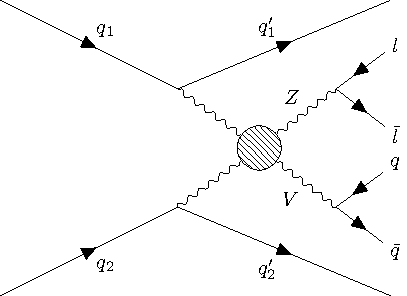
\includegraphics[width=\textwidth]{figures/feyn_vbs_0.pdf}
    \vspace{5pt}
  \end{minipage}
  \begin{minipage}{0.23\textwidth}
    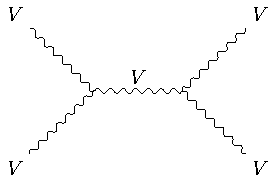
\includegraphics[width=\textwidth]{figures/feyn_vbs_2.pdf}
  \end{minipage}%
  \begin{minipage}{0.18\textwidth}
    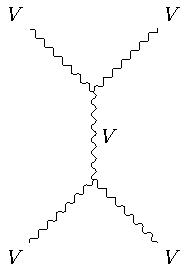
\includegraphics[width=\textwidth]{figures/feyn_vbs_4.pdf}
  \end{minipage}%
  \begin{minipage}{0.23\textwidth}
    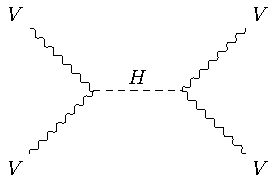
\includegraphics[width=\textwidth]{figures/feyn_vbs_3.pdf}
  \end{minipage}%
  \begin{minipage}{0.18\textwidth}
    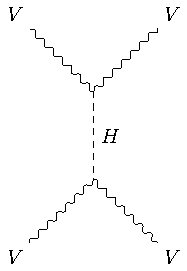
\includegraphics[width=\textwidth]{figures/feyn_vbs_5.pdf}
  \end{minipage}%
  \begin{minipage}{0.16\textwidth}
    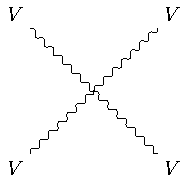
\includegraphics[width=\textwidth]{figures/feyn_vbs_1.pdf}
  \end{minipage}
  \caption[Tree level Feynman diagram of ZV VBS process at LHC]%
  {Tree level Feynman diagram of ZV VBS process at LHC\@. The top diagram
    shows the production of two vector boson being radiated from incoming
    quarks, in final state after scattering (blob), Z decays
    to pair of leptons, V (W/Z) decays to pair of quarks,
    and plus two outgoing quarks.
    The bottom row of diagram shows the tree
    level processes that can happen in scattering represented by blob in
    top diagram, starting from s and t-channel exchange of
    vector boson, Higgs boson, and the last one is quartic
    coupling of vector bosons.
  }%
  \label{fig:feynman-vbs}
\end{figure}
\chapter{
  The LHC and CMS Experiment
 }\label{ch_cms}

The physics analysis is carried out using data collected by the \gls{CMS} experiment at
\gls{CERN} \gls{LHC} accelerator. This chapter provides overview of the \gls{LHC}
and details of the CMS experiment and its sub-detectors for particle tracking
and calorimetry.

\section{
  The Large Hadron Collider
 }\label{ch_cms:lhc}

The \gls{LHC} is the largest proton-proton
collider, located at
\gls{CERN} in Geneva, Switzerland.
The main \gls{LHC} ring is 27\km{} in circumference
and 50 to 175\m{} underground.
The \gls{LHC} is built to collide protons at 14\TeV{} center-of-mass energy,
LHC delivered proton-proton collisions at 7 and 8\TeV{}
during run1 (2010--2012), and at 13\TeV{} center-of-mass energy during
run2 (2015--2018)
~\cite{Evans:2008}.

Figure~\ref{fig:lhc} describes \gls{CERN} accelerator complex.
The protons are sourced by ionizing hydrogen atoms
and then fed into a \gls{LINAC}.
The \gls{LINAC} accelerates the protons to 50\MeV{} and delivers them to the booster.
Then the booster increases the energy of the protons to 1.4\GeV{} and
feeds them to the \gls{PS} which further increases their energy to 25\GeV{}
and starts bunching them together with bunches 25\nanoseconds{} apart.
The proton bunches are passed through \gls{SPS} which brings their energy
to 450\GeV{} and bunches are then finally sent to main \gls{LHC} clockwise and counterclockwise
rings where they are accelerated to final energy required which is 6.5\TeV{}
for both bunches going clockwise and counterclockwise
to obtain collisions at 13\TeV{} center-of-mass energy.

The proton-proton collisions occurs, at four different locations where two
general purpose detectors \gls{CMS} and \gls{ATLAS}, and
two specific purpose detector \gls{ALICE} and \gls{LHCb} are located.

\begin{figure}[!ht]
  \centering
  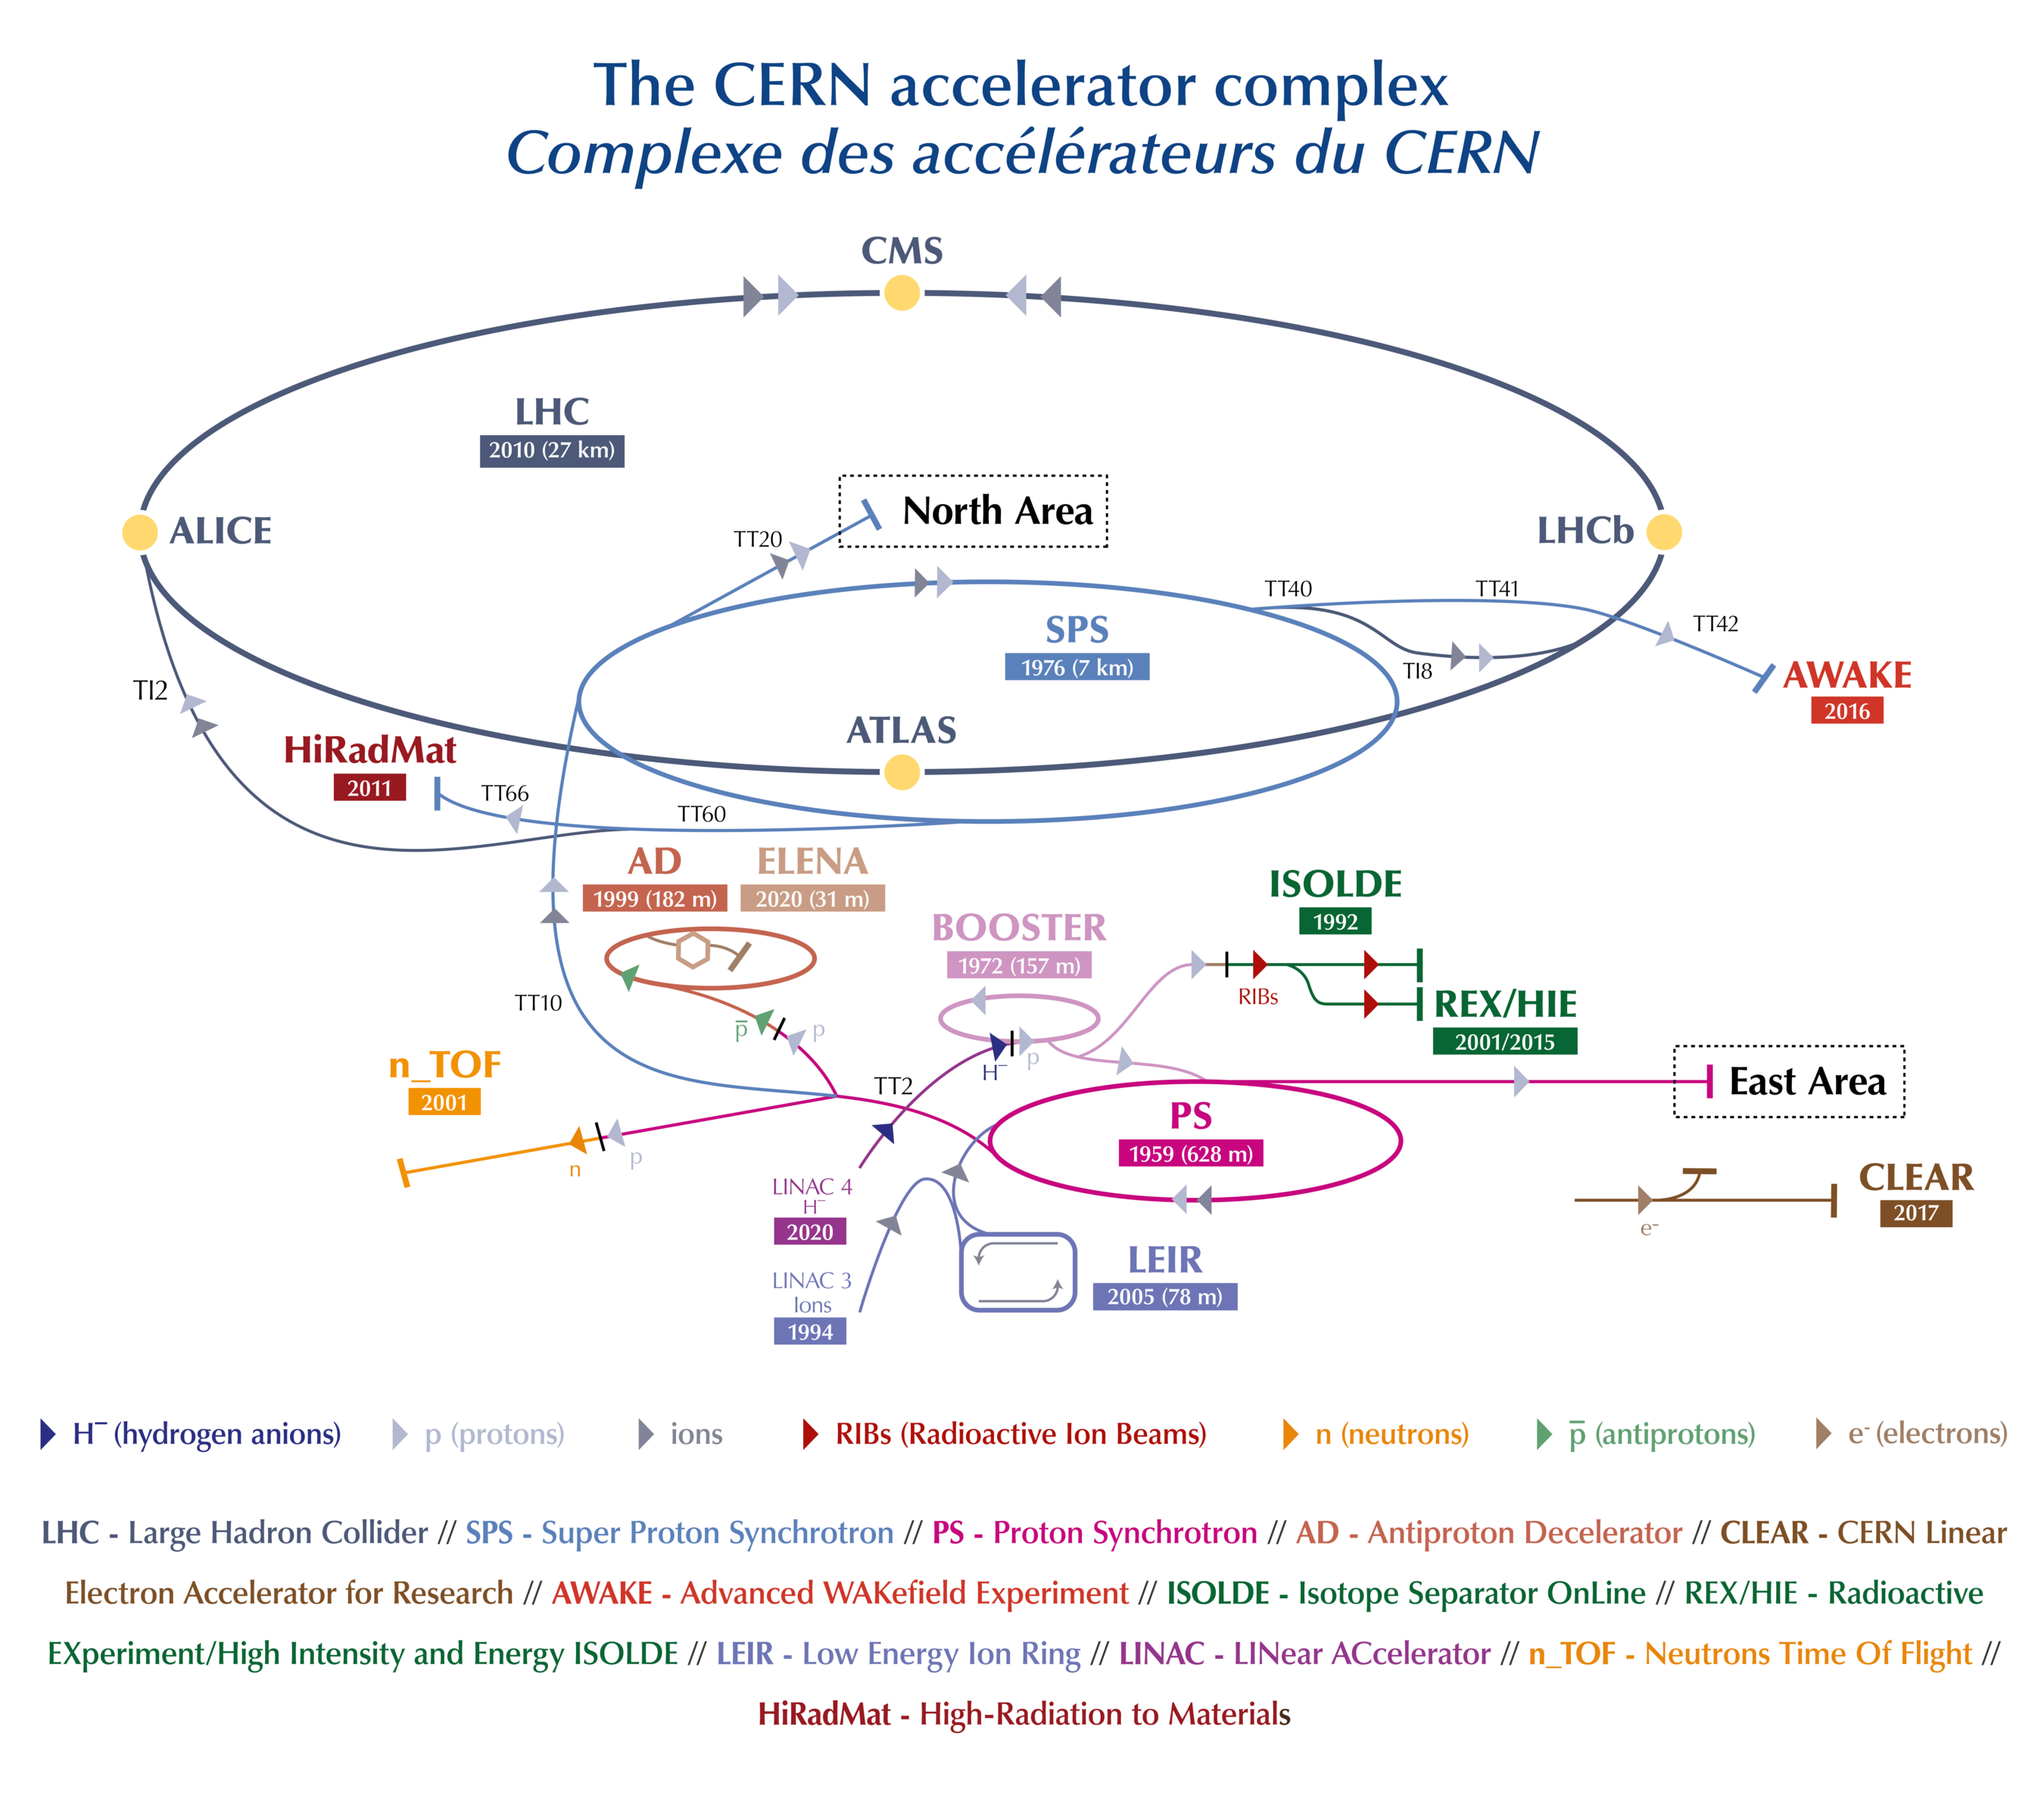
\includegraphics[width=0.98\textwidth]{figures/lhc-scheme.png}
  \caption[A schematic of the CERN accelerator complex]%
  {A schematic of the CERN accelerator complex~\cite{image-lhc-scheme}}%
  \label{fig:lhc}
\end{figure}

\subsection{
  Integrated Luminosity
}\label{ch_cms:cms-lumi}

Luminosity is a measure of how many events can happen per unit area and per
unit time for a collision or scattering process, and it is defined as,
%
\begin{equation}
  L = \frac{1}{\sigma} \frac{dN}{dt}, \quad L_{\text{int}} = \int L dt
\end{equation}

where \(\sigma \) is cross-section of the process
and \(L\) is the instantaneous luminosity (\( \cm{}^{-2} \seconds^{-1} \)),
and \( L_{\text{int}} \) is the integrated luminosity usually
expressed in inverse units of cross-section (\pbinv{}, \fbinv{}, etc.).

For proton-proton collision at \gls{LHC}
the nominal instantaneous luminosity is of the order of \( 10^{34} \cm{}^{-2} \seconds^{-1}\),
and integrated luminosity delivered and recorded by \gls{CMS} during run2\footnote{2\textsuperscript{nd} run period (2015--2018) of proton-proton collisions at LHC} operation
is shown in Figure~\ref{fig:int-lumi}.

\begin{figure}[!ht]
  \centering
  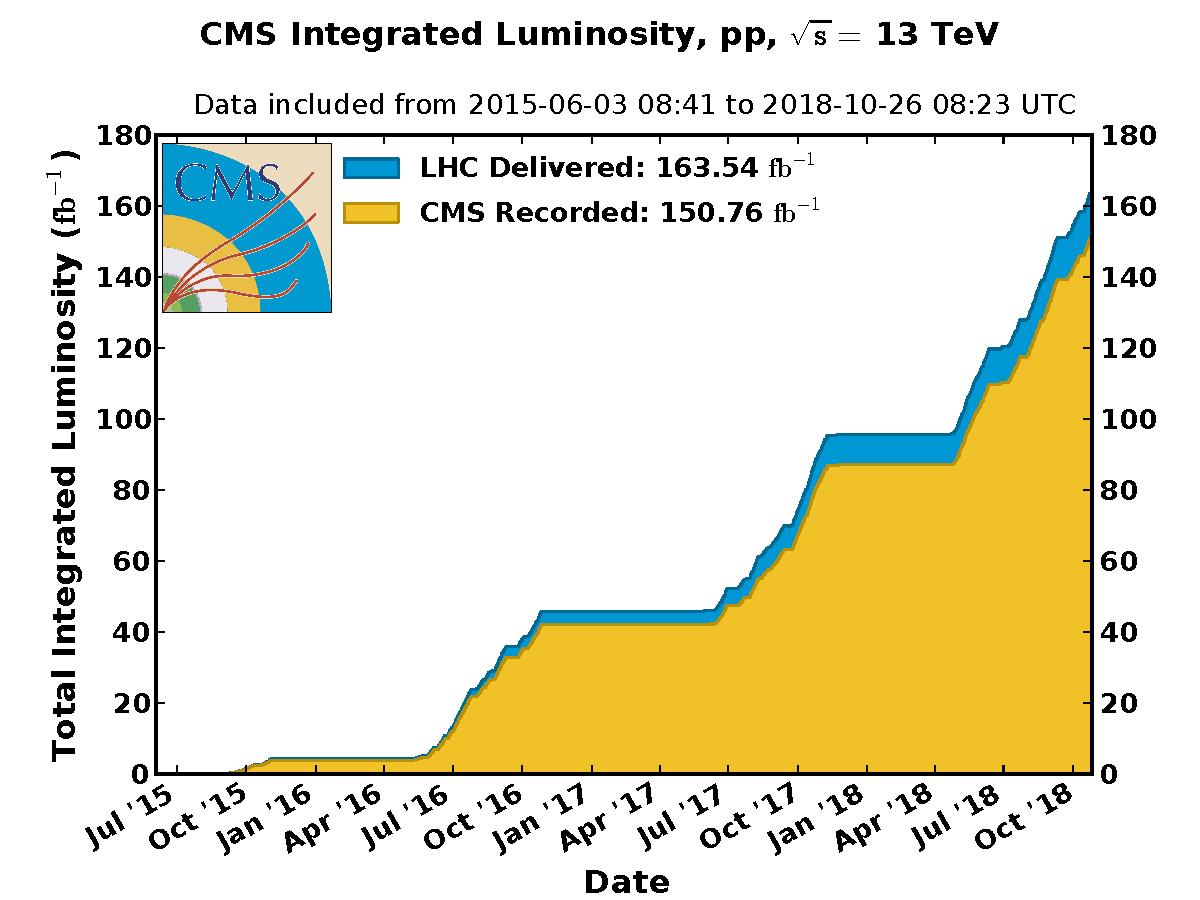
\includegraphics[width=0.60\textwidth]{figures/int_lumi_pp_run2.pdf}
  \caption[Integrated delivered and recorded luminosity
    for 2015--2018 proton-proton collisions]%
  {Integrated delivered and recorded luminosity
    for  2015--2018 proton-proton collisions~\cite{plot-cms-lumi}}%
  \label{fig:int-lumi}
\end{figure}

For run2 standard physics analysis, luminosity recorded during
2016--2018 years is considered, and only runs certified as ``golden'' by \gls{CMS}
Luminosity \gls{POG} are used for the analysis. The runs
are certified as ``golden'' if all the subdetector, triggers and
physics objects perform as expected. The total
integrated luminosity for run2
standard physics is 137.19\fbinv{} (35.92\fbinv{} during 2016, 41.53\fbinv{}
during 2017, and 59.74\fbinv{} during 2018 period)
~\cite{CMS-PAS-LUM-17-001,CMS-PAS-LUM-17-004,CMS-PAS-LUM-18-002}.

\section{
  The CMS Detector
 }\label{ch_cms:cms}

The \gls{CMS} detector is a general purpose high energy particle physics detector.
A cutaway view of the detector is shown in Figure~\ref{fig:cms-cutaway}.
The detector is cylindrical with dimensions: 21 meters long, and 15 meters
in diameter, with the whole detector weighing about 14000 tonnes.
The detector is built in slices with central region called the ``barrel'',
and the two enclosing sides called ``endcaps''.
A superconducting solenoid generates magnetic field of 3.8\Tesla{} inside
and 2\Tesla{} outside. To contain the magnetic field outside of solenoid
and support structure of the detector, massive steel yokes are used.

\begin{figure}[!ht]
  \centering
  \includegraphics[width=\textwidth]{figures/cms_cutway_ME4_2.pdf}
  \caption[The CMS detector cutaway view]%
  {The CMS detector cutaway view~\cite{image-cms-cutway}}%
  \label{fig:cms-cutaway}
\end{figure}

Figure~\ref{fig:cms-slice} shows a schematic view of the \gls{CMS} detector, and
how different particles leave signature in various sub-detectors.
Neutral particles such as photons, neutrinos, and neutral hadrons will leave no track
in the \gls{ST}, and are identified only by the energy deposited
in the calorimeters or the missing energy in an event.
Electrons are identified from the track in the \gls{ST} and energy deposit
in the \gls{ECAL}. Since hadrons are heavier and they pass through the \gls{ECAL}
and deposit their most of energy in the \gls{HCAL}, leaving only small fraction
of energy in the \gls{ECAL}.
Since muons are \glspl{MIP}, they pass through whole detector with very small
fraction of the energy deposited in the \gls{ECAL} and \gls{HCAL}.

This following section gives an overview of the subsystems of \gls{CMS} detector.
For detailed technical description refer to~\cite{CMS-JINST-S08004}.

\begin{figure}[!ht]
  \centering
  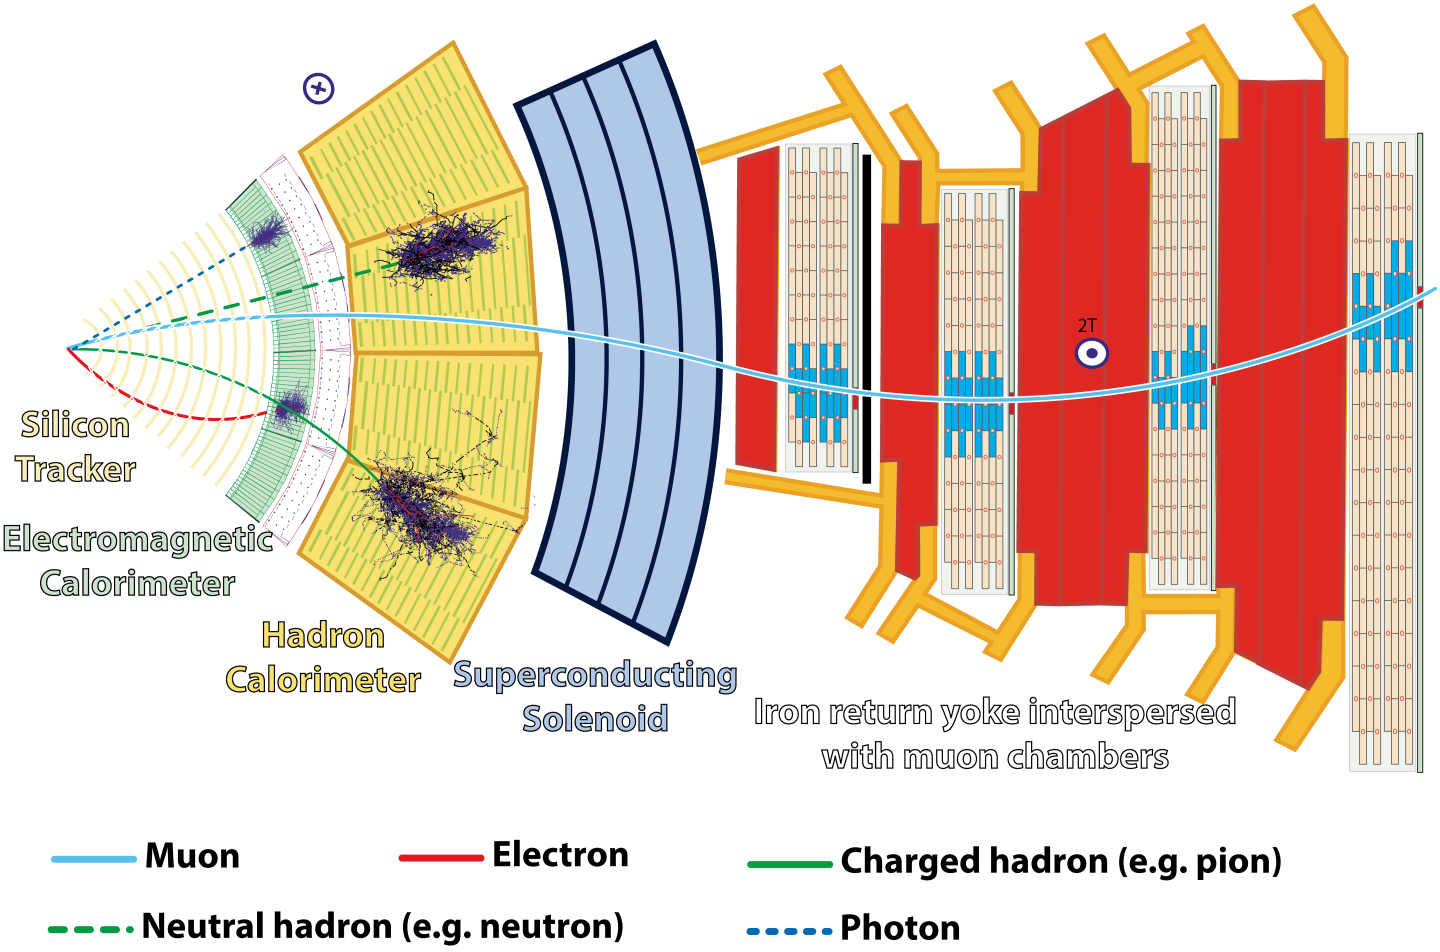
\includegraphics[width=\textwidth]{figures/cms_slice.png}
  \caption[Schematic view of the CMS detector]%
  {Schematic view of the CMS detector~\cite{image-cms-slice}}%
  \label{fig:cms-slice}
\end{figure}

\clearpage{}
\subsection{
  The CMS Coordinate System
}\label{ch_cms:cms-coordinate}

CMS uses \gls{IP} of the collisions as origin to define the right-handed
coordinate system. The \( z \)-axis is along the beamline,
the \( x \)-axis points toward the center of the \gls{LHC},
and the \( y \)-axis points upwards toward the Earth's surface.
The transverse plane \( x - y \) is used to calculate
most commonly used quantities like transverse momentum \( p_{T} \)
and energy \( E_{T} \).

To describe the direction of particles leaving the \gls{IP},
azimuthal \( \phi \) and polar \( \theta \) angles are used.
\( \phi \) is measured around the beam axis,
and \( \theta \) is measured from the beam axis.
In collider physics, pseudorapidity \( \eta \) (Lorentz invariant) is used
to describe direction from beam pipe instead of \( \theta \) as,
%
\begin{equation}
  \eta = - \ln[\tan{\theta/2}]
\end{equation}

and sometimes in terms of rapidity \( y \) as,
%
\begin{equation}
  y = \frac{1}{2} \ln{\frac{E+p_{z}}{E-p_{z}}}
\end{equation}

Particle kinematics can be completely described in terms of
\( p_{T} \), \( \eta \), \( \phi \), and \( E_{T} \) or mass.
The distance between the two particles in \( \eta - \phi \) plane
is described as \( \Delta R \),
%
\begin{equation}
  \Delta R = \sqrt{ {(\Delta \eta)}^{2} + {(\Delta \phi)}^{2} }
\end{equation}

\subsection{
  The Superconducting Magnet
}

The superconducting magnet is the central part of the \gls{CMS} detector, it is
12.5 meters long and 6.3 meters in diameter. The magnet is cooled to
4.5\,\text{K}\xspace and a 20\,\text{kA}\xspace current flows through it to
generate 3.8\Tesla{} of magnetic field with stored energy of 2.6\,\text{GJ}\xspace.

Figure~\ref{fig:cms-magnet} shows the
installation (in 2007) of the superconducting magnet with iron yoke in the underground
cavern.

The key purpose of the magnet is to help determine the momentum and the sign of charged
particles by bending them. The momentum resolution of the particles
decreases with increase in their \(p_T \). Constant magnetic field of 3.8\Tesla{}
gives momentum resolution of \(\Delta p /p \approx 10 \% \). This resolution
is enough to determine unambiguously the sign of muons with
momentum of \(\approx 1\TeV{}/c \).

\begin{figure}[!ht]
  \centering
  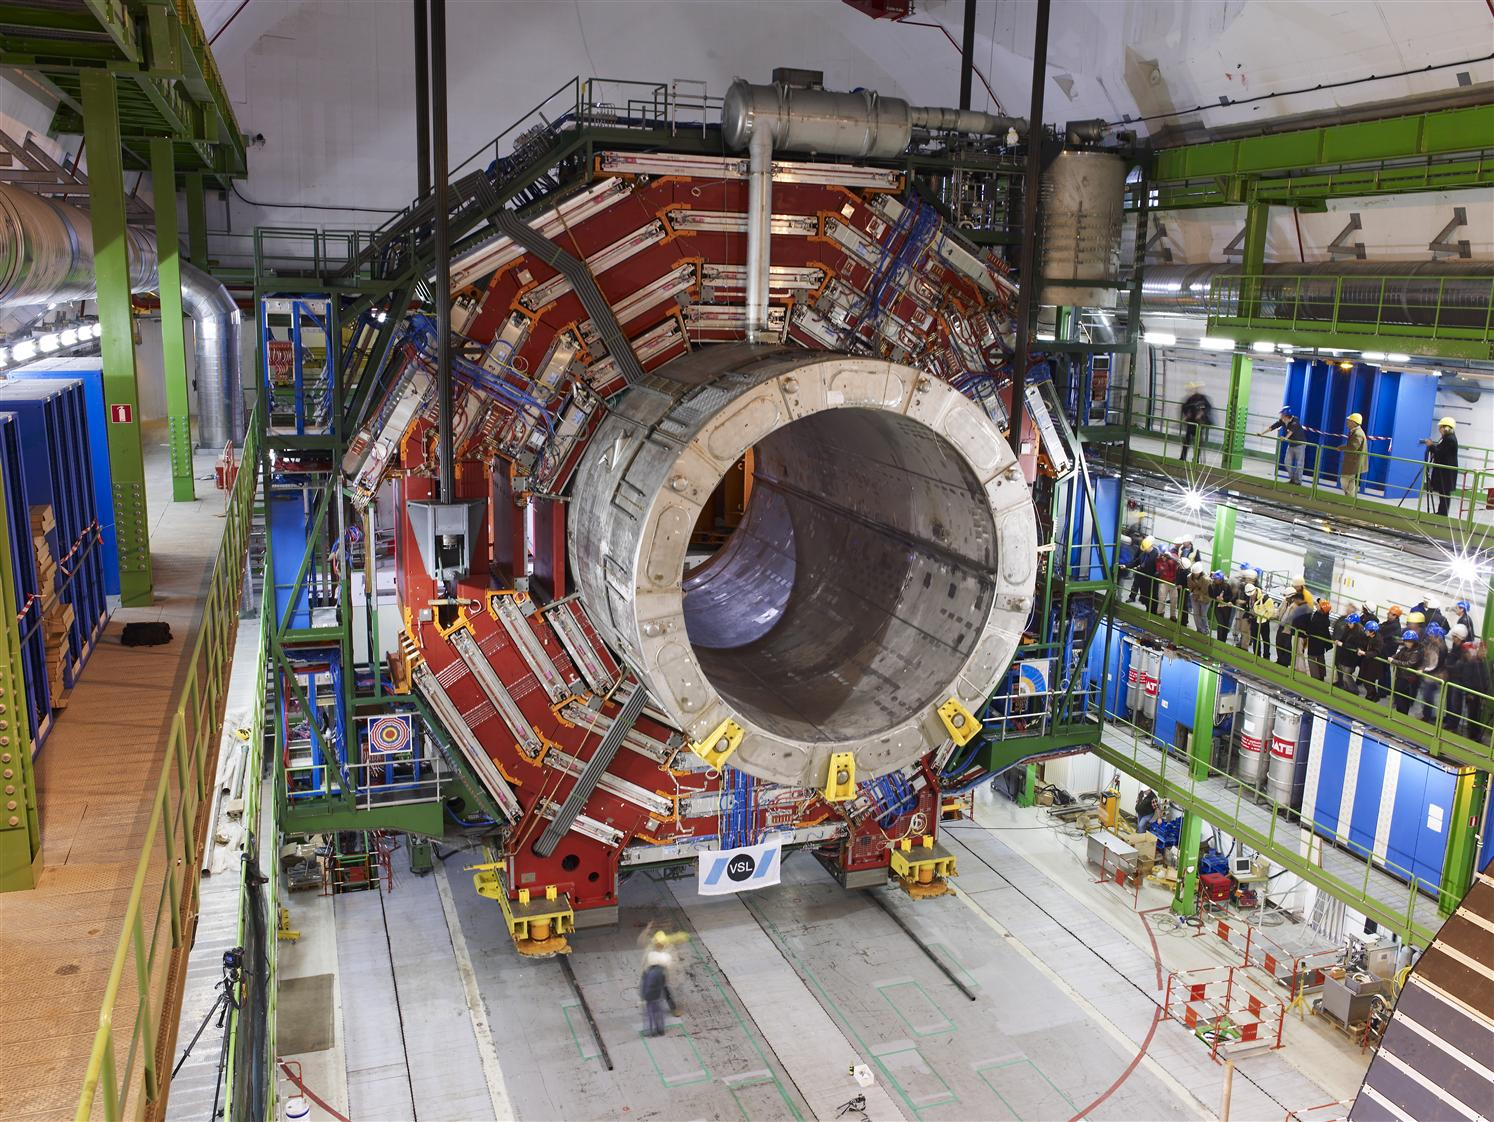
\includegraphics[width=0.75\textwidth]{figures/cms_magnet_lowered.jpg}
  \caption%
  [The picture of the CMS detector central part when lowered in underground
    cavern with superconducting magnet and iron
    yoke]%
  {The picture of the CMS detector central part when lowered in underground
    cavern with superconducting magnet and iron
    yoke~\cite{image-cms-magnet}.}%
  \label{fig:cms-magnet}
\end{figure}


\subsection{
  The Tracking System
}

The \gls{CMS} tracking system \gls{ST} is the innermost part of the detector, it
is made up of pixel and strip detectors. The main goal of \gls{ST} is to
reconstruct the tracks of the charged particles with high precision in high pileup
environment.

Silicon is most commonly used material for making tracking systems because of it's
semiconductor properties, and high radiation hardness which is essential for the
innermost detector. When a p-n junction is built on silicon substrate it creates
a depletion zone with no charge carriers at the junction, and whenever
a charged particle passes through the depletion zone it creates a electron-hole pair.
Under reverse bias this electron-hole generates an electrical signal. The \gls{CMS}
tracker consists of about 124 million channels of such junctions in the
pixel detector and 10 million in the strip detector.

The pixel detector was upgraded in 2017 and the comparison of layers before
and after the upgrade is shown in Figure~\ref{fig:cms-pixel}. It is made up of
four barrel layers and three endcaps, with nearest barrel layer being 3\cm{}
away from the beamline for precise measurement of the \gls{IP}.
Because of the large number of pixel channels, the readout is done by \glspl{ASIC}.

\begin{figure}[!ht]
  \centering
  \begin{minipage}[c]{.62\textwidth}
    \includegraphics[trim={80pt 0 80pt 0},clip,width=\textwidth]%
    {figures/cms_pixel_phase1.pdf}
  \end{minipage}
  \begin{minipage}[c]{.35\textwidth}
    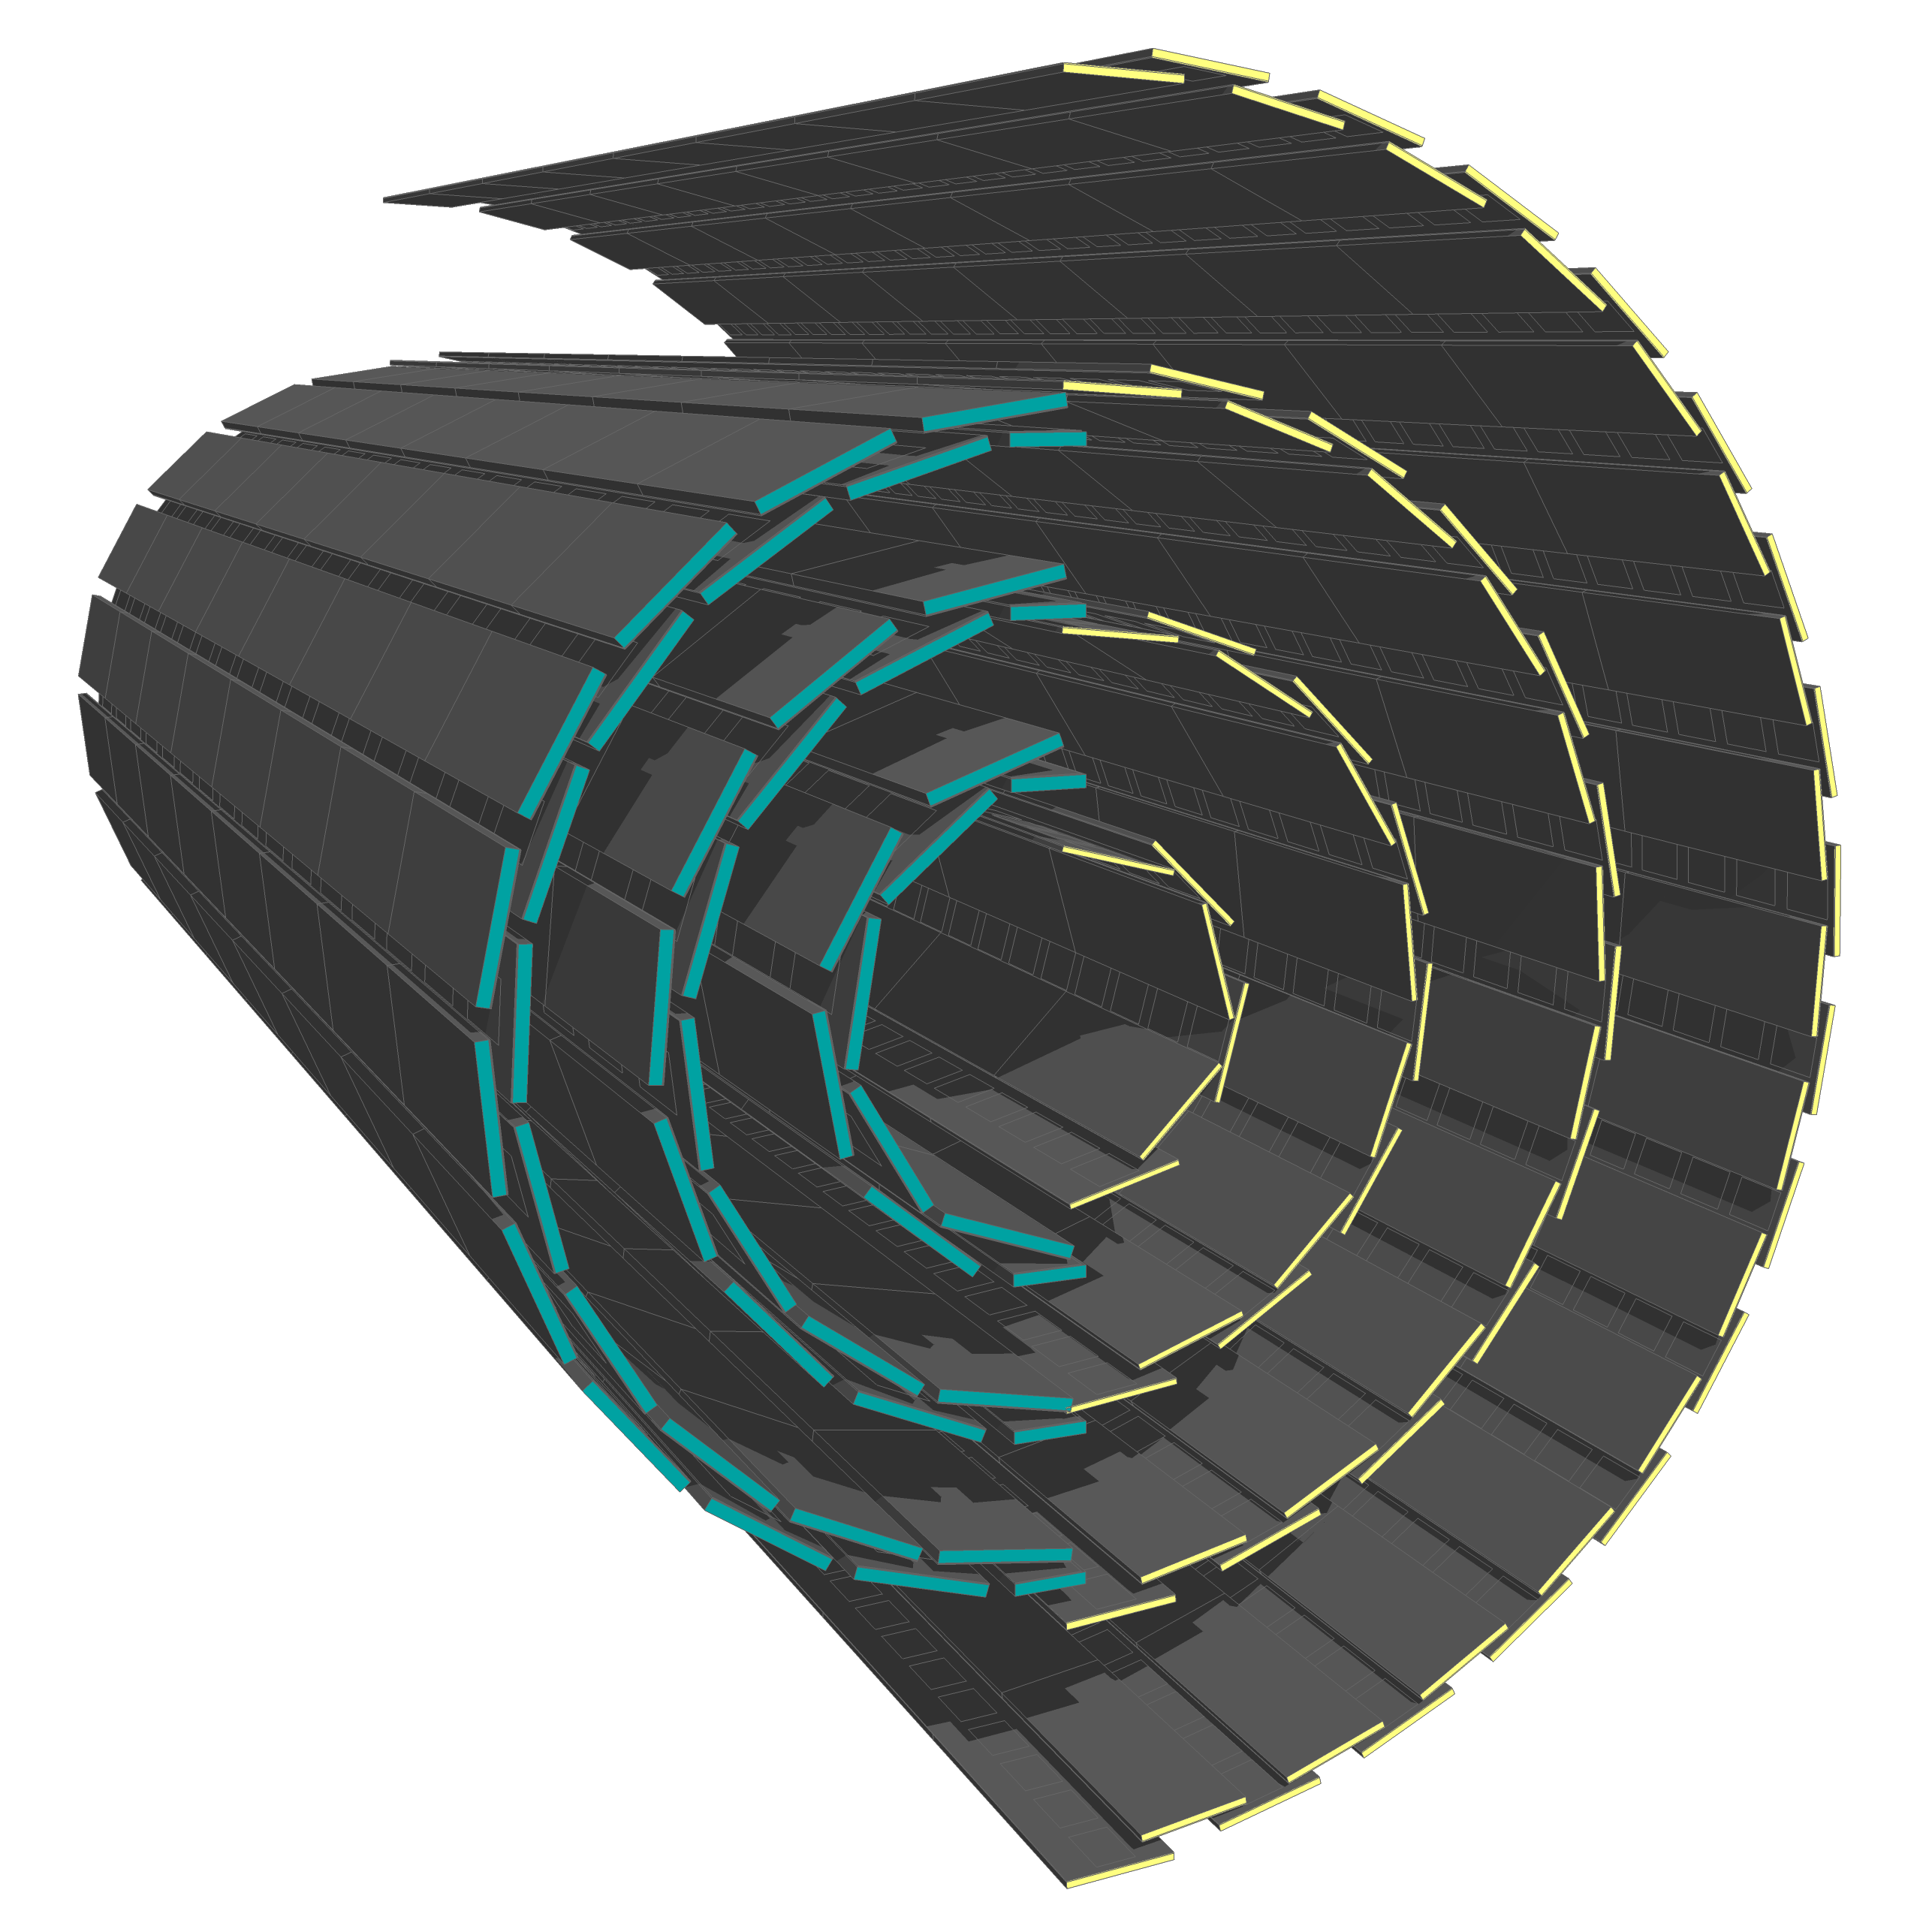
\includegraphics[width=\textwidth]{figures/cms_pixel_phase1_04.png}
  \end{minipage}
  \caption[The CMS pixel upgrade]%
  {The CMS pixel upgrade. The left is cross sectional view of pixel detector
    layers before upgrade (bottom) and after Phase 1 upgrade (top).
    The right is view pixel barrel before upgrade (left)
    and after upgrade (right)~\cite{image-cms-pixel}.}%
  \label{fig:cms-pixel}
\end{figure}

The outermost part of \gls{ST} detector is made up of silicon strips. It allows for large
coverage by reducing number of readout channels. It has 10 layers in barrel region
and 12 discs in endcap region. For better signal-to-noise ratio and radiation
tolerance both pixel and strip detector are operated at -20\,\de\text{C}\xspace.

\subsection{
  The Electromagnetic Calorimeter
}

The \gls{ECAL} active material is made of lead tungstate (PbWO\textsubscript{4})
scintillating crystals and two layers silicon strip for preshower
in front of the endcaps. The crystals in central barrel section are mounted
in quasi-projective geometry pointing towards \gls{IP} and cover
\( |\eta| < 1.48 \). The two endcaps extends the coverage to
\( |\eta| = 3.0 \). The schematic layout of \gls{ECAL} is shown in Figure~\ref{fig:cms-ecal-schematic}
and the picture of endcap quadrant when assembled is shown in Figure~\ref{fig:cms-ecal-ee}

The main purpose of the \gls{ECAL} is to determine energy and positions of
electromagnetically interacting particles.
Except electron and photons all other particles pass
through \gls{ECAL} crystals with only small fraction of energy signature in the crystals.
When electron and photon interacts with PbWO\textsubscript{4} it starts an process
of electromagnetic shower which continues until the energy the energy of the incident
particle is below threshold, which is about 1\MeV{}.

\begin{figure}[!ht]
  \centering
  \begin{minipage}[c]{.60\textwidth}
    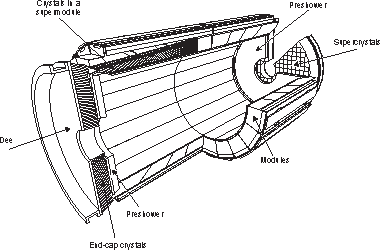
\includegraphics[width=\textwidth]{figures/cms_ecal_schematic.pdf}
  \end{minipage}
  \begin{minipage}[c]{.38\textwidth}
    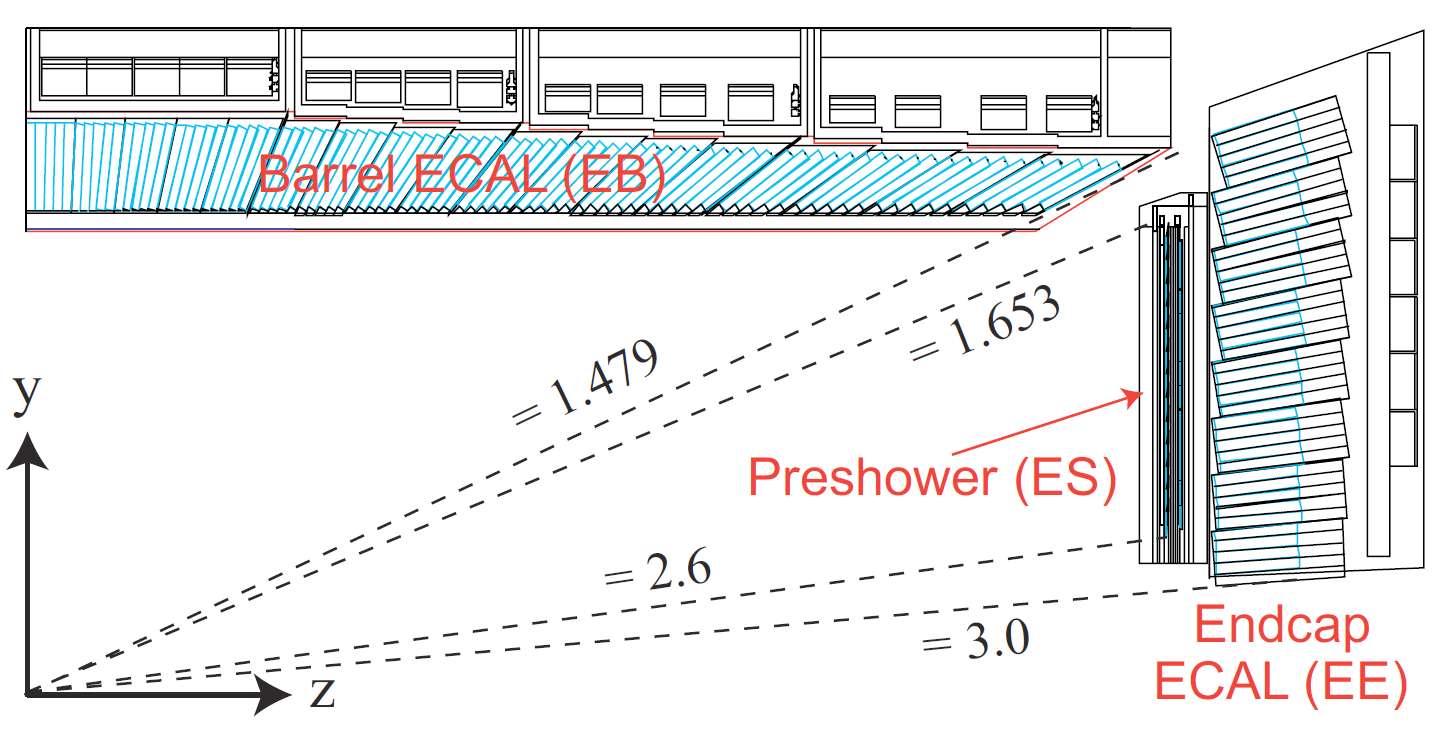
\includegraphics[width=\textwidth]{figures/cms_ecal_layout.png}
  \end{minipage}
  \caption[The CMS \gls{ECAL} schematic layout]%
  {The \gls{CMS} \gls{ECAL} schematic layout. The left schematic shows the arrangement of
    superclusters in barrel and endcap (with preshower layers). On the right is the \(y-z \)
    plane quarter view of \gls{ECAL} layout~\cite{image-cms-ecal-layout}.}%
  \label{fig:cms-ecal-schematic}
\end{figure}

\begin{figure}[!ht]
  \centering
  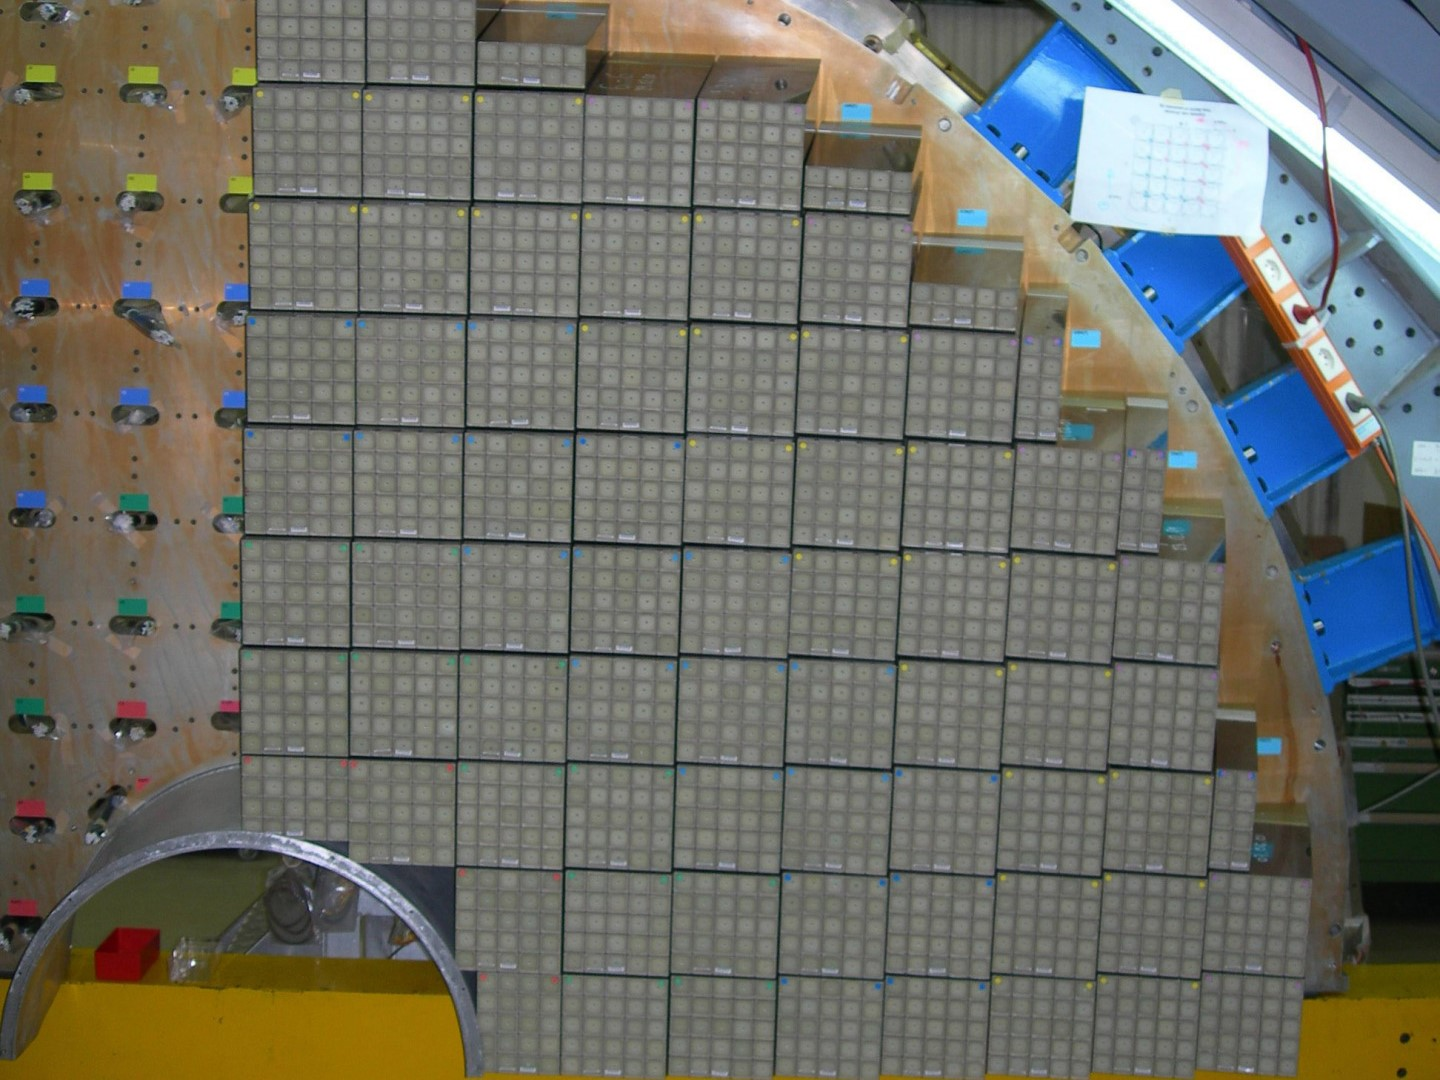
\includegraphics[width=0.60\textwidth]{figures/cms_ecal_ee_quadrant.jpg}
  \caption[The \gls{ECAL} endcap quadrant assembled view]%
  {The \gls{ECAL} endcap quadrant assembled view~\cite{image-cms-ecal-ee-quadrant}.}%
  \label{fig:cms-ecal-ee}
\end{figure}

The fractional resolution of the \gls{ECAL} energy measurements can be described as,
%
\begin{equation}
  {\left( \frac{\sigma}{E} \right)}^2
  = {\left( \frac{S}{\sqrt{E}} \right)}^2
  + {\left( \frac{N}{E} \right)}^2
  + C^2
\end{equation}

where \(S \) is the stochastic term, \(N \) is related to the noise,
and C is a constant offset. The energy resolution in the central
region of \gls{ECAL} barrel (\( |\eta| < 0.8 \)) for electrons from \textit{Z}
decays was 2\% and 2--5\% elsewhere. The energy resolution for photons
from Higgs decay varied from 1.1\% to 2.6\% in the barrel region and
from 2.2\% to 5\% in the endcaps~\cite{energy-ecal-7tev}.

\subsection{
  The Hadronic Calorimeter
}

Similar to \gls{ECAL}, the purpose of \gls{HCAL}
is to shower hadrons, and measure their energy and position.
The first half of barrel \gls{HCAL} inserted into solenoid during installation
is shown in Figure~\ref{fig:cms-hcal-inserted}.

\gls{HCAL} is made up of
towers pointing towards \gls{IP} where each tower is made up of sampling layers;
with alternating layers of plastic scintillator and brass.
Brass acts as absorber in the \gls{HCAL} and causes hadrons to shower.
Scintillators emits light when secondary particles
from hadronic shower pass through them.
The light output collected from the scintillator layers, combined with
total absorption length of Brass layers
gives the total energy deposited in the \gls{HCAL}.
In phase 1 upgrade the \gls{HCAL} was upgraded
to give energy deposit as a function of depth.
The depth segmentation schematic is
show in Figure~\ref{fig:cms-hcal-depth} and the details of upgrade are in technical design
report~\cite{cms-hcal-upgrade}.

\begin{figure}[!ht]
  \centering
  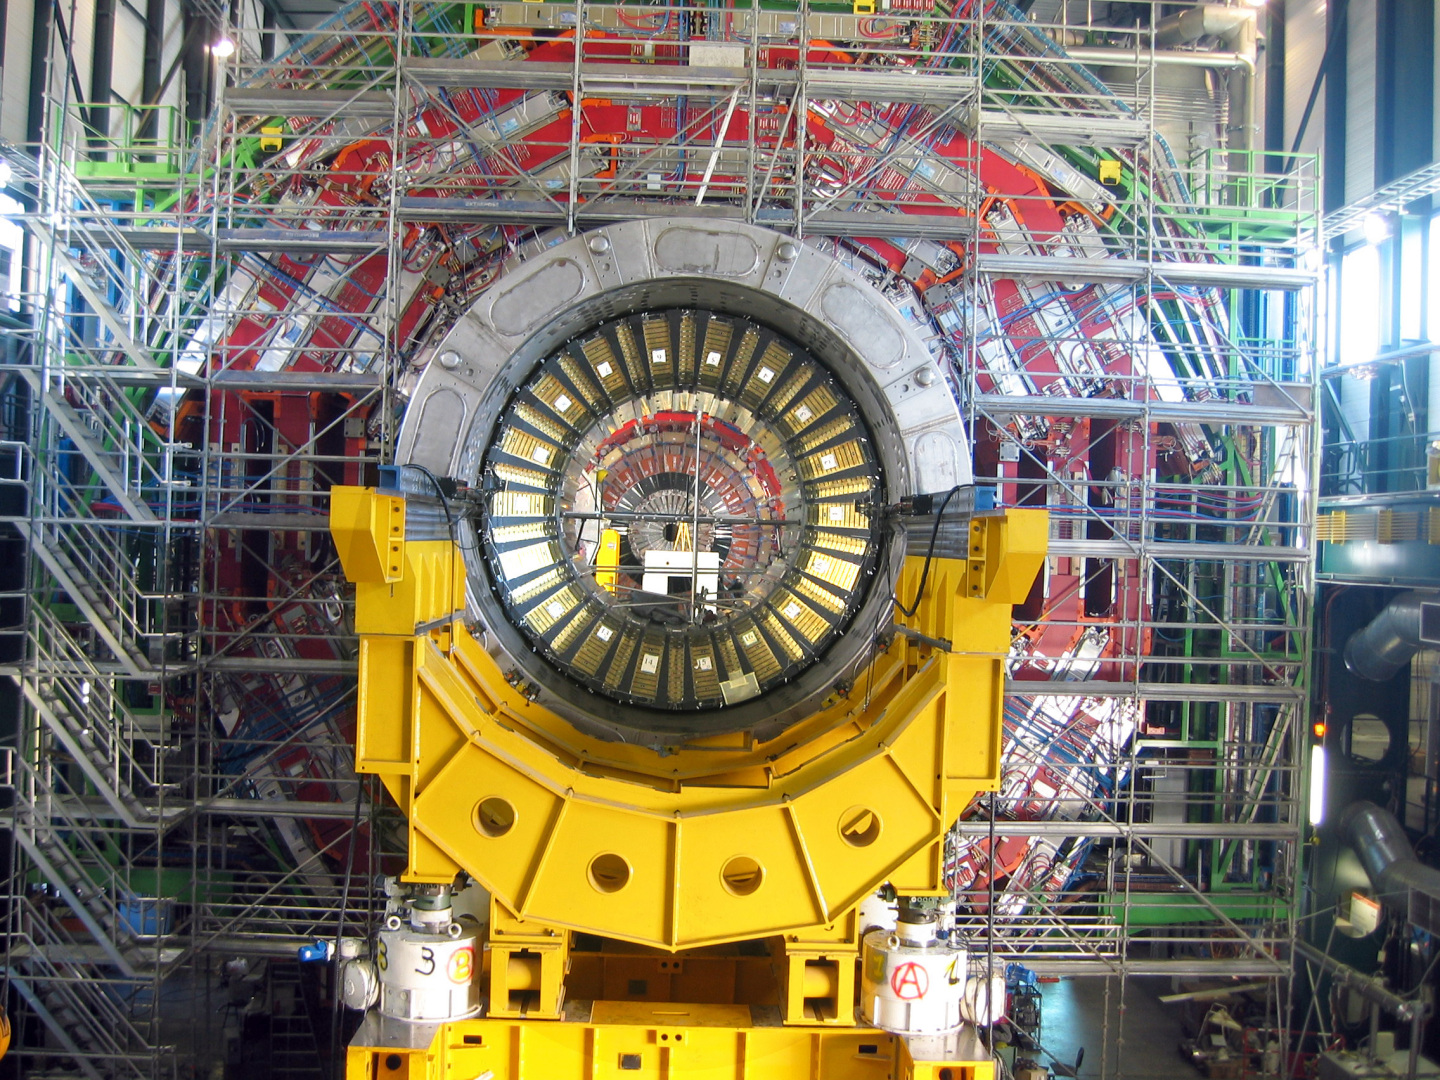
\includegraphics[width=\textwidth]{figures/cms_hcal_hb_inserted.jpg}
  \caption[The first half of the barrel \gls{HCAL} inserted into the
    superconducting solenoid (April 2006)]%
  {The first half of the barrel \gls{HCAL} inserted into the
    superconducting solenoid (April 2006)~\cite{image-cms-hcal-inserted}.}%
  \label{fig:cms-hcal-inserted}
\end{figure}

\gls{HCAL} consists barrel (HB) and two endcaps (HE) located inside solenoid.
These two subsystems combined provides
coverage of \( |\eta| \le 3.0 \).
There are two other subsystems of \gls{HCAL} outside solenoid,
a forward \gls{HCAL} (HF) and outer barrel \gls{HCAL} (HO).
HO was added to ensure there is no leakage from the particles that
make it past the solenoid. HF extends the coverage
to \(|\eta| \le 5.0\). HF is based on Cherenkov radiation principle
and uses quartz fiber as active material with steel absorbers.

\begin{figure}[!ht]
  \centering
  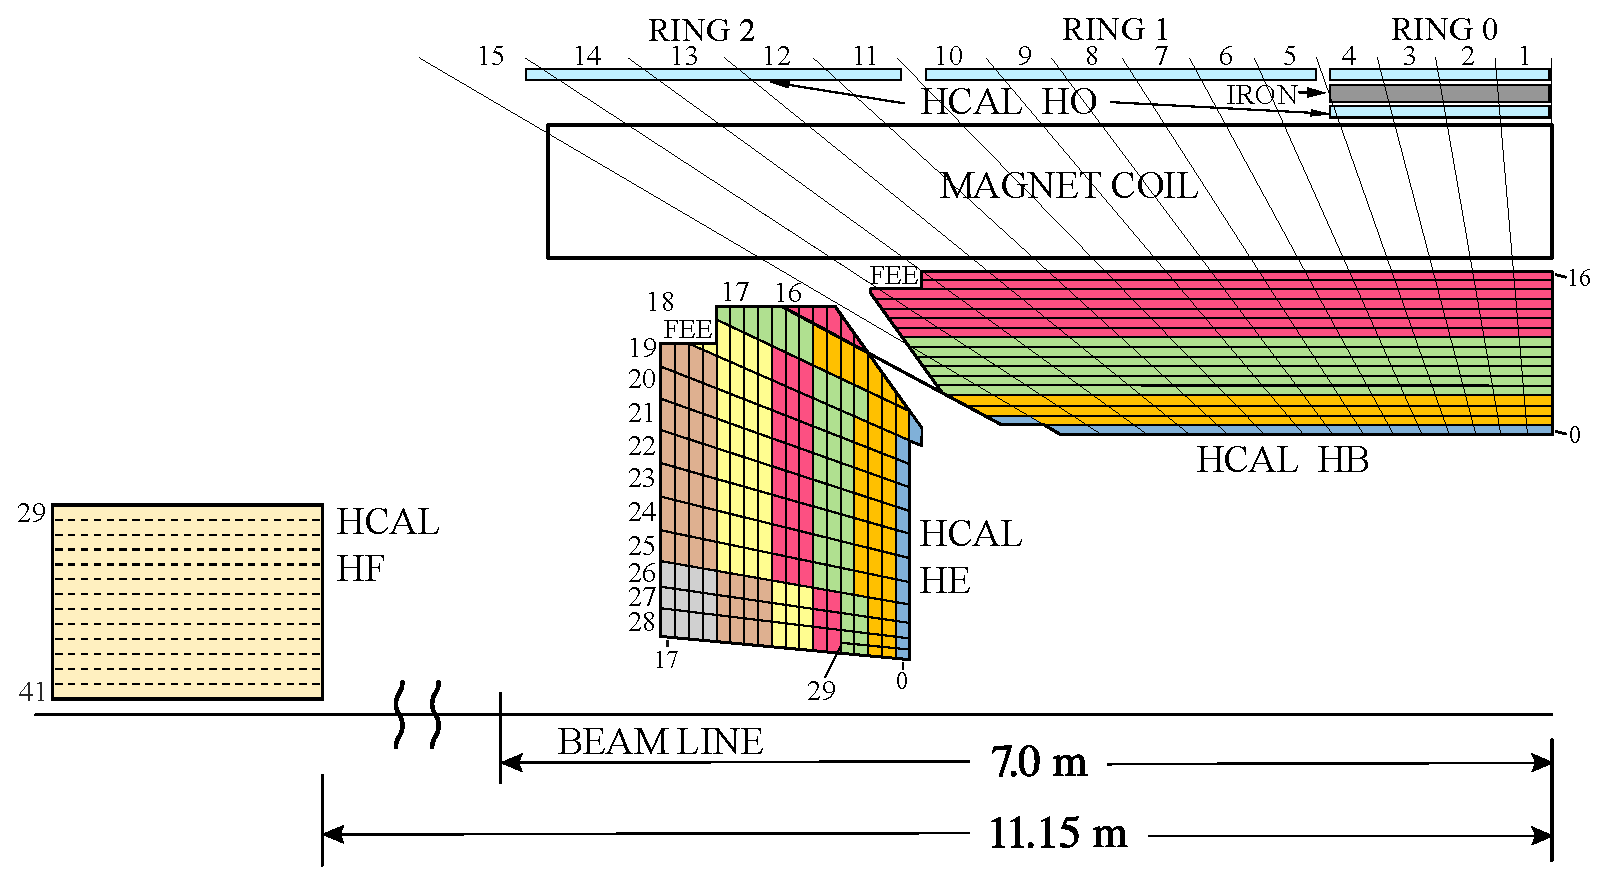
\includegraphics[width=\textwidth]{figures/cms_hcal_depth_seg.pdf}
  \caption[The \gls{HCAL} depth segmentation after phase 1 upgrade]%
  {The \gls{HCAL} depth segmentation after phase 1 upgrade~\cite{image-cms-hcal-depth}.}%
  \label{fig:cms-hcal-depth}
\end{figure}

\subsection{
  Muon Detector
}

The outermost subsystem in the \gls{CMS} detector is the muon detector.
Unlike electrons, muons are \glspl{MIP} i.e.
they do not lose much of their energy
while passing through tracker, calorimeter and solenoid.
Muon detector is built to identify, measure momentum and trigger the events
with muons. Like other subsystems, the muon detector consists of a barrel and endcap
detector. The schematic layout is highlighted in the Figure~\ref{fig:cms-muon-system}.
As shown in the schematic, the muon detector consists of three subsystems \glspl{DT}, \glspl{CSC} and
\glspl{RPC}.

The \glspl{DT} are wire gas detectors filled with Argon and composed of
many tube cells of about 4\cm{}. Muon passing through these tubes
ionize Argon and the free electron is detected on the wire cathode.
Each DT is about 2 meters by 2.5 meters in size, and there are four layers
of the \glspl{DT} interleaved with the iron yoke, parallel to
the beam pipe in barrel region. The drift time is the order of about 380\nanoseconds.

\begin{figure}[!ht]
  \centering
  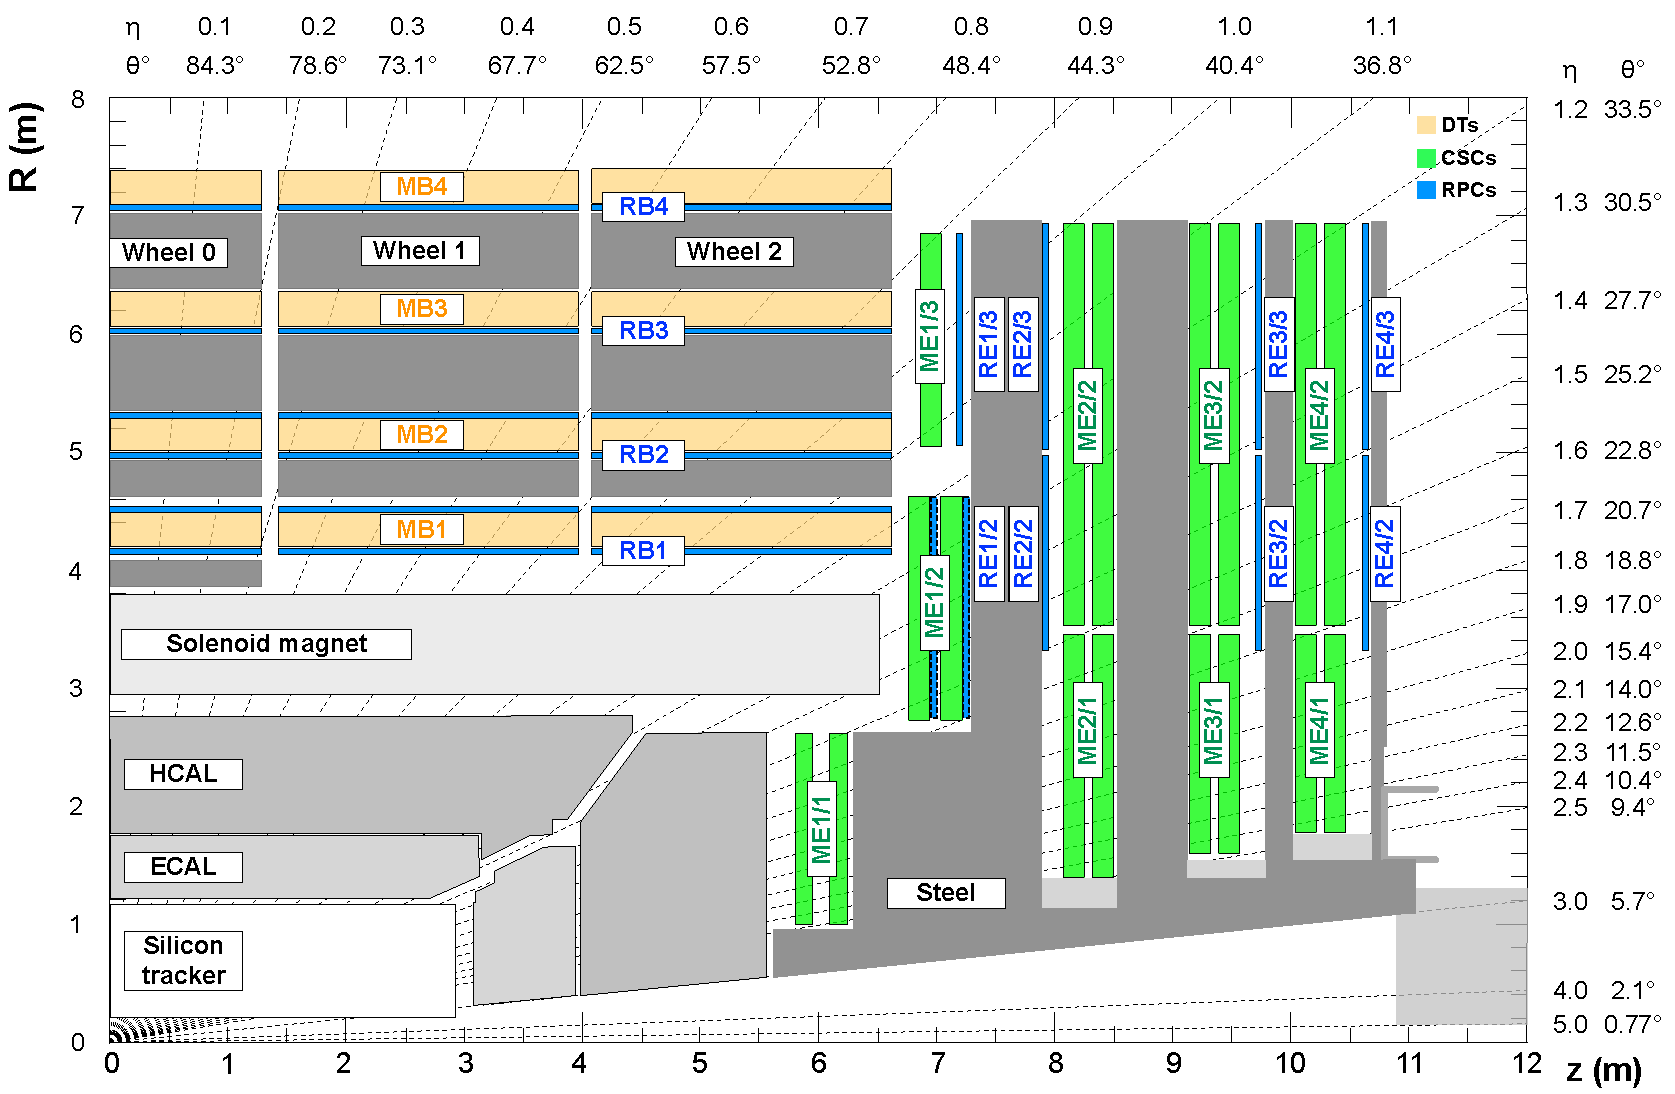
\includegraphics[width=0.9\textwidth]{figures/cms_muon_system.pdf}
  \caption[The quadrant view of CMS subdetectors layout, and
    the coverage of the muon detector \glspl{DT}, \glspl{CSC},
    and \glspl{RPC} highlighted]%
  {The quadrant view of CMS subdetectors layout, and
    the coverage of the muon detector \glspl{DT}, \glspl{CSC},
    and \glspl{RPC} highlighted~\cite{image-cms-muon-system}.}%
  \label{fig:cms-muon-system}
\end{figure}

The \glspl{CSC} are based on same principle as \glspl{DT},
and are made of multi-wire proportional chambers consisting of
6 anode planes interleaved with 7 cathode planes. They have time resolution
better than 5\nanoseconds. The \glspl{CSC} are used in endcap region,
where radiation hardness is required, and non uniform magnetic field does not
effects the measurement.

The \glspl{RPC} are made up of two oppositely charged high resistive parallel
plates with a gas\footnote{mixture of 96.2\% \( C_{2}H_{2}F_{4} \), 3.5\% Iso-\( C_{4}H_{10} \),
0.3\% \( S{F}_{6} \)} volume between them.
When a charged particles passes through, it ionizes the gas, and it creates
an avalanche. The charge is collected by metallic readout strips.
\glspl{RPC} have poor position resolution but fast readout of the order of 1\nanoseconds,
which is fast compared to \glspl{DT}, this is the reason there are 1 or 2 \glspl{RPC}
attached to both \glspl{DT}, and \glspl{CSC}.

\subsection{
  Trigger
}\label{ch_cms:L1T}

Since proton-proton collisions occurs every bunch crossing which are
25\nanoseconds{} apart; equivalent to a 40\,\text{MHz}\xspace collisions rate.
At this collisions rate, the data storage required will be enormous
and \gls{CMS} can only record up to 1000 events per second. Since most of events
do not contain interesting physics events, they can be thrown away.
To do this \gls{CMS} has two tier trigger system \gls{L1T}, and \gls{HLT}.

The \gls{L1T} is the first electronic processing system through
which event information is processed before it is passed to
second trigger system: \gls{HLT}.
The \gls{L1T} is designed to make fast decisions in about 3.8\mus,
and only uses \gls{ECAL}, \gls{HCAL} and muon system to make a decision
regarding throwing or keeping an event.
\gls{L1T} cut downs the data rate from 40\,\text{MHz}\xspace to
100\,\text{kHz}\xspace. The \gls{L1T} electronics is placed next to
the detector in underground cavern for fast transfer of data.

Events accepted by \gls{L1T} are passed to the \gls{HLT}.
The \gls{HLT} further reduces the data rate from 100\,\text{kHz}\xspace to
about 1\,\text{kHz}\xspace using a computer farm with nearly 26000 cores.
\gls{HLT} uses all the available information from the event to make
decision in about 300 ms. \gls{HLT} is modular by design
to allow the use of information from different systems to construct
multiple paths called \gls{HLT} paths, for example the single muon \gls{HLT}
path will save event with at least one muon passing the selection criteria
set in \gls{HLT} path. Events passing at least on \gls{HLT} path are
saved for offline physics analysis.

\chapter{
  Event Simulation and Reconstruction
 }\label{ch_reco}

The proton-proton collision at \gls{LHC} produces shower of particles, before
the event information can be easily used in an analysis, the data collected goes
through iterative process of reconstruct particles produced in collision.
\gls{CMS} uses \gls{PF} algorithm to reconstruct 4-vectors of muons, electrons,
photons, hadrons, jets and missing transverse momentum~\cite{cms-particle-flow-2017}.

To analyze the data collected and compare it with theoretical model, events are
simulated using \gls{MC} event generators and are passed through detector simulation
and \gls{PF} so that \gls{MC} events can be treated same as real events.

This chapter describes the basic ingredients for object reconstruction, \gls{PF}
candidates and \gls{MC} event generators used in this analysis.

\section{
  Track Reconstruction
 }

\gls{KF}~\cite{cms-track-reco} \GEANTfour{}

\section{
  Calorimeter Clustering
 }

\section{
  Particles Flow Candidates
 }

\subsection{
  Muons
}

\subsection{
  Electrons and Photons
}

\subsection{
  Hadrons and Jets
}

\subsection{
  Missing transverse momentum
}

\section{
  Monte Carlo Simulation
 }

\subsection{
  Generators
}

\subsection{
  Hadronization
}

\chapter{
  VBS Measurement in ZVjj Final State
 }\label{ch_vbs}

As discussed in Section~\ref{ch_intro:vbs} this analysis targets
\gls{VBS} of ZV with two jets in final state. The goal of the analysis
is to reduce contribution from background processes as much as possible
without loosing much of signal, and measure signal strength and significance.

Since Z decays leptonically and V is decaying hadronically,
the phase-space of this analysis can be either
\( l^+ l^- jjjj \) or \( l^+ l^- J jj\), where \( l \) are leptons,
\( j \) are narrow jets and \( J \) is a boosted (wider) jet.
The phase-space is divided into two broad regions signal and controlled,
signal region is constructed based on theory such that it is mostly signal process
and controlled region is basically orthogonal to the signal region
where we expect contributions mostly from background processes.

The analysis is performed ``blind'' to avoid intrinsic bias
i.e.\ until the analysis procedure is finalized, the collision data is only used
in controlled regions. Once the analysis technique is optimized using \gls{MC}
samples and validated against collision data in controlled regions. Once the
analysis technique is satisfactory and approved by \gls{CMS} Physics Group
then the results are ``un-blinded'' i.e.\ measurements are done
using collision data in signal region.

\section{
  Dataset and Simulation
 }

As discussed in Section~\ref{ch_cms:L1T} only events those pass Level-1
Trigger and \gls{HLT} paths are saved for further processing, \gls{MC}
simulation also have these identical step during event generation to mimic
Level-1 Trigger and \gls{HLT} paths.

\gls{CMS} collaboration processes the datasets centrally and provides various
tiers of datasets such as ``RECO'' datasets, which contains reconstructed
objects and no skimming. Average size of an event saved at ``RECO'' tier is
480 kB per event and on average an analysis will process
3 billion events, which makes this tier not practical in terms of computer processing
time and storage if each analysis starts from ``RECO''. \gls{CMS} centrally
processes these datasets further and removes certain objects
or features to reduce the average event size but still covering
majority of the analysis to make use of the reduced datasets.

This analysis uses \NanoAOD{} tier with version ``v7'' of datasets
which has average event size of 2--3 kB.

\subsection{
  Data
}

The collision data events used in this analysis are all certified
by \gls{CMS} \gls{DQM} and \gls{DC} group. The primary trigger object in
\gls{HLT} paths are leptons \( p_{T} \) threshold, and since in our final state
we are looking for Z boson decaying into two leptons, we require single and
double lepton trigger for our analysis. Depending on the detector
conditions and \gls{LHC} storage capacity we have slightly different threshold
in triggers across different years. The Table~\ref{tab:hlt-paths} contains the list of
\gls{HLT} paths used in this analysis.

\begin{table}[!ht]
  \centering
  \caption{Trigger paths used to select events in CMS collision data}
  \begin{tabular}{cll}%
    \toprule
    Dataset & Year                  & HLT Path                                          \\
    \midrule
    \multirow{4}{*}{Single Muon}
            & \multirow{2}{*}{2016} & \url{HLT_IsoMu24}                                 \\
            &                       & \url{HLT_IsoTkMu24}                               \\
    \cmidrule(lr){2-3}
            & \multirow{1}{*}{2017} & \url{HLT_IsoMu27}                                 \\
    \cmidrule(lr){2-3}
            & \multirow{1}{*}{2018} & \url{HLT_IsoMu24}                                 \\
    \midrule
    \multirow{4}{*}{Single Electron}
            & \multirow{2}{*}{2016} & \url{HLT_Ele27_WPTight_Gsf}                       \\
            &                       & \url{HLT_Ele25_eta2p1_WPTight_Gsf}                \\
    \cmidrule(lr){2-3}
            & \multirow{1}{*}{2017} & \url{HLT_Ele35_WPTight_Gsf}                       \\
    \cmidrule(lr){2-3}
            & \multirow{1}{*}{2018} & \url{HLT_Ele32_WPTight_Gsf}                       \\
    \midrule
    \multirow{6}{*}{Double Muon}
            & \multirow{3}{*}{2016} & \url{HLT_Mu17_TrkIsoVVL_Mu8_TrkIsoVVL_DZ}         \\
            &                       & \url{HLT_Mu17_TrkIsoVVL_TkMu8_TrkIsoVVL_DZ}       \\
            &                       & \url{HLT_TkMu17_TrkIsoVVL_TkMu8_TrkIsoVVL_DZ}     \\
    \cmidrule(lr){2-3}
            & \multirow{2}{*}{2017} & \url{HLT_Mu17_TrkIsoVVL_Mu8_TrkIsoVVL_DZ_Mass8}   \\
            &                       & \url{HLT_Mu17_TrkIsoVVL_Mu8_TrkIsoVVL_DZ_Mass3p8} \\
    \cmidrule(lr){2-3}
            & \multirow{1}{*}{2018} & \url{HLT_Mu17_TrkIsoVVL_Mu8_TrkIsoVVL_DZ_Mass3p8} \\
    \midrule
    \multirow{4}{*}{Double Electron}
            & \multirow{2}{*}{2016} & \url{HLT_Ele23_Ele12_CaloIdL_TrackIdL_IsoVL_DZ}   \\
            &                       & \url{HLT_Ele23_Ele12_CaloIdL_TrackIdL_IsoVL}      \\
    \cmidrule(lr){2-3}
            & \multirow{1}{*}{2017} & \url{HLT_Ele23_Ele12_CaloIdL_TrackIdL_IsoVL}      \\
    \cmidrule(lr){2-3}
            & \multirow{1}{*}{2018} & \url{HLT_Ele23_Ele12_CaloIdL_TrackIdL_IsoVL}      \\
    \bottomrule
  \end{tabular}\label{tab:hlt-paths}
\end{table}

\subsection{
  MC Simulations
}

The \gls{EW} \gls{VBS} process which is our signal is
generated with \MADGRAPH{}5+\PYTHIA{}8 at \gls{LO} with \( \alpha_{EW}^{6} \) order
i.e.
all vertices in tree level Feynman diagram are \gls{EW} vertices.
The \gls{QCD} induced \gls{VBS} background process which is very
similar to our signal is generated with same configuration
but with \( \alpha_{EW}^{4} \alpha_{QCD}^{2} \) order i.e.
two of the six vertices are \gls{QCD}. The dominant background to analysis
\gls{DY} + Jets and, top-quark based processes consisting of
single top-quark (t and s-channel),
single top-quark in association with W boson (tW) and top-quark pair (t\=t) production.
The \gls{DY} + Jets are generated at \gls{LO} with \MADGRAPH{}5+\PYTHIA{}8
in bins of HT i.e.
scalar sum of all the jets \( p_{T} \) in the event, to have more statistics
for higher HT bins. Top-quark background process are generated at \gls{NNLO},
s-channel is generated with \MADGRAPH{}\_\MCATNLO{}5+\PYTHIA{}8 and others
t-channel, tW, t\=t are generated with \POWHEG{}+\PYTHIA{}8.
The complete list of Table~\ref{tab:mc-list-1},~\ref{tab:mc-list-2},~\ref{tab:mc-list-3} contains
the list of Signal and Background MC samples used for modeling in this analysis.

\begin{sidewaystable}[!ht]
  \centering
  \caption{List of MC samples for Signal and Background modeling}
  \resizebox{\textwidth}{!}{%
    \begin{tabular}{llll}%
      \toprule
      Process & Year       & Dataset Name                                                                      & Cross Section (pb) \\
      \midrule
      \midrule
      \multirow{6}{1.1in}{
        VBS\_EWK (Signal)}
              & 2016       & \url{WminusTo2JZTo2LJJ_EWK_LO_SM_MJJ100PTJ10_TuneCUETP8M1_13TeV-madgraph-pythia8} & 0.02982            \\
              & 2016       & \url{WplusTo2JZTo2LJJ_EWK_LO_SM_MJJ100PTJ10_TuneCUETP8M1_13TeV-madgraph-pythia8}  & 0.05401            \\
              & 2016       & \url{ZTo2LZTo2JJJ_EWK_LO_SM_MJJ100PTJ10_TuneCUETP8M1_13TeV-madgraph-pythia8}      & 0.01589            \\
      \cmidrule(lr){2-4}
              & 2017, 2018 & \url{WminusTo2JZTo2LJJ_EWK_LO_SM_MJJ100PTJ10_TuneCP5_13TeV-madgraph-pythia8}      & 0.02982            \\
              & 2017, 2018 & \url{WplusTo2JZTo2LJJ_EWK_LO_SM_MJJ100PTJ10_TuneCP5_13TeV-madgraph-pythia8}       & 0.05401            \\
              & 2017, 2018 & \url{ZTo2LZTo2JJJ_EWK_LO_SM_MJJ100PTJ10_TuneCP5_13TeV-madgraph-pythia8}           & 0.01589            \\
      \midrule
      \midrule
      \multirow{6}{1.1in}{
        VBS\_QCD (Background)}
              & 2016       & \url{WminusTo2JZTo2LJJ_QCD_LO_SM_MJJ100PTJ10_TuneCUETP8M1_13TeV-madgraph-pythia8} & 0.3488             \\
              & 2016       & \url{WplusTo2JZTo2LJJ_QCD_LO_SM_MJJ100PTJ10_TuneCUETP8M1_13TeV-madgraph-pythia8}  & 0.575              \\
              & 2016       & \url{ZTo2LZTo2JJJ_QCD_LO_SM_MJJ100PTJ10_TuneCUETP8M1_13TeV-madgraph-pythia8}      & 0.3449             \\
      \cmidrule(lr){2-4}
              & 2017, 2018 & \url{WminusTo2JZTo2LJJ_QCD_LO_SM_MJJ100PTJ10_TuneCP5_13TeV-madgraph-pythia8}      & 0.3488             \\
              & 2017, 2018 & \url{WplusTo2JZTo2LJJ_QCD_LO_SM_MJJ100PTJ10_TuneCP5_13TeV-madgraph-pythia8}       & 0.575              \\
              & 2017, 2018 & \url{ZTo2LZTo2JJJ_QCD_LO_SM_MJJ100PTJ10_TuneCP5_13TeV-madgraph-pythia8}           & 0.3449             \\
      \midrule
      \midrule
      \multirow{16}{1.1in}{
        DY + Jets LO (Background)}
              & 2016       & \url{DYJetsToLL_M-50_HT-70to100_TuneCUETP8M1_13TeV-madgraphMLM-pythia8}           & 169.9              \\
              & 2016       & \url{DYJetsToLL_M-50_HT-100to200_TuneCUETP8M1_13TeV-madgraphMLM-pythia8}          & 147.4              \\
              & 2016       & \url{DYJetsToLL_M-50_HT-200to400_TuneCUETP8M1_13TeV-madgraphMLM-pythia8}          & 41.04              \\
              & 2016       & \url{DYJetsToLL_M-50_HT-400to600_TuneCUETP8M1_13TeV-madgraphMLM-pythia8}          & 5.674              \\
              & 2016       & \url{DYJetsToLL_M-50_HT-600to800_TuneCUETP8M1_13TeV-madgraphMLM-pythia8}          & 1.358              \\
              & 2016       & \url{DYJetsToLL_M-50_HT-800to1200_TuneCUETP8M1_13TeV-madgraphMLM-pythia8}         & 0.6229             \\
              & 2016       & \url{DYJetsToLL_M-50_HT-1200to2500_TuneCUETP8M1_13TeV-madgraphMLM-pythia8}        & 0.1512             \\
              & 2016       & \url{DYJetsToLL_M-50_HT-2500toInf_TuneCUETP8M1_13TeV-madgraphMLM-pythia8}         & 0.003659           \\
      \cmidrule(lr){2-4}
              & 2017       & \url{DYJetsToLL_M-50_HT-70to100_TuneCP5_13TeV-madgraphMLM-pythia8}                & 167.33             \\
              & 2017       & \url{DYJetsToLL_M-50_HT-100to200_TuneCP5_13TeV-madgraphMLM-pythia8}               & 161.1              \\
              & 2017       & \url{DYJetsToLL_M-50_HT-200to400_TuneCP5_13TeV-madgraphMLM-pythia8}               & 48.66              \\
              & 2017       & \url{DYJetsToLL_M-50_HT-400to600_TuneCP5_13TeV-madgraphMLM-pythia8}               & 6.968              \\
              & 2017       & \url{DYJetsToLL_M-50_HT-600to800_TuneCP5_13TeV-madgraphMLM-pythia8}               & 1.743              \\
              & 2017       & \url{DYJetsToLL_M-50_HT-800to1200_TuneCP5_13TeV-madgraphMLM-pythia8}              & 0.8052             \\
              & 2017       & \url{DYJetsToLL_M-50_HT-1200to2500_TuneCP5_13TeV-madgraphMLM-pythia8}             & 0.1933             \\
              & 2017       & \url{DYJetsToLL_M-50_HT-2500toInf_TuneCP5_13TeV-madgraphMLM-pythia8}              & 0.003468           \\
      \bottomrule
    \end{tabular}%
  }\label{tab:mc-list-1}
\end{sidewaystable}

\begin{sidewaystable}[!ht]
  \centering
  \caption{List of MC samples for Signal and Background modeling}
  \resizebox{\textwidth}{!}{%
    \begin{tabular}{llll}%
      \toprule
      Process & Year & Dataset Name                                                                         & Cross Section (pb) \\
      \midrule
      \midrule
      \multirow{8}{1.1in}{
        DY + Jets LO (Background)}
              & 2018 & \url{DYJetsToLL_M-50_HT-70to100_TuneCP5_PSweights_13TeV-madgraphMLM-pythia8}         & 167.33             \\
              & 2018 & \url{DYJetsToLL_M-50_HT-100to200_TuneCP5_PSweights_13TeV-madgraphMLM-pythia8}        & 161.1              \\
              & 2018 & \url{DYJetsToLL_M-50_HT-200to400_TuneCP5_PSweights_13TeV-madgraphMLM-pythia8}        & 48.66              \\
              & 2018 & \url{DYJetsToLL_M-50_HT-400to600_TuneCP5_PSweights_13TeV-madgraphMLM-pythia8}        & 6.968              \\
              & 2018 & \url{DYJetsToLL_M-50_HT-600to800_TuneCP5_PSweights_13TeV-madgraphMLM-pythia8}        & 1.743              \\
              & 2018 & \url{DYJetsToLL_M-50_HT-800to1200_TuneCP5_PSweights_13TeV-madgraphMLM-pythia8}       & 0.8052             \\
              & 2018 & \url{DYJetsToLL_M-50_HT-1200to2500_TuneCP5_PSweights_13TeV-madgraphMLM-pythia8}      & 0.1933             \\
              & 2018 & \url{DYJetsToLL_M-50_HT-2500toInf_TuneCP5_PSweights_13TeV-madgraphMLM-pythia8}       & 0.003468           \\
      \midrule
      \midrule
      \multirow{21}{1.1in}{
        Top (Background)}
              & 2016 & \url{ST_tW_antitop_5f_NoFullyHadronicDecays_13TeV_PSweights-powheg-pythia8}          & 38.06              \\
              & 2016 & \url{ST_tW_antitop_5f_inclusiveDecays_TuneCP5_PSweights_13TeV-powheg-pythia8}        & 34.97              \\
              & 2016 & \url{ST_tW_top_5f_NoFullyHadronicDecays_13TeV_PSweights-powheg-pythia8}              & 38.09              \\
              & 2016 & \url{ST_tW_top_5f_inclusiveDecays_TuneCP5_PSweights_13TeV-powheg-pythia8}            & 34.91              \\
              & 2016 & \url{ST_t-channel_antitop_4f_InclusiveDecays_TuneCP5_PSweights_13TeV-powheg-pythia8} & 67.91              \\
              & 2016 & \url{ST_t-channel_top_4f_InclusiveDecays_TuneCP5_PSweights_13TeV-powheg-pythia8}     & 113.3              \\
              & 2016 & \url{ST_s-channel_4f_leptonDecays_13TeV_PSweights-amcatnlo-pythia8}                  & 3.365              \\
              & 2016 & \url{ST_s-channel_4f_hadronicDecays_TuneCP5_PSweights_13TeV-amcatnlo-pythia8}        & 11.24              \\
              & 2016 & \url{ST_s-channel_4f_InclusiveDecays_13TeV-amcatnlo-pythia8}                         & 10.12              \\
              & 2016 & \url{TTToHadronic_TuneCP5_PSweights_13TeV-powheg-pythia8}                            & 377.96             \\
              & 2016 & \url{TTToSemiLeptonic_TuneCP5_PSweights_13TeV-powheg-pythia8}                        & 365.34             \\
              & 2016 & \url{TTTo2L2Nu_TuneCP5_PSweights_13TeV-powheg-pythia8}                               & 88.29              \\
      \cmidrule(lr){2-4}
              & 2017 & \url{TTToSemiLeptonic_TuneCP5_13TeV-powheg-pythia8}                                  & 365.34             \\
              & 2017 & \url{TTTo2L2Nu_TuneCP5_13TeV-powheg-pythia8}                                         & 86.99              \\
              & 2017 & \url{TTToHadronic_TuneCP5_13TeV-powheg-pythia8}                                      & 377.96             \\
              & 2017 & \url{ST_s-channel_antitop_leptonDecays_13TeV-PSweights_powheg-pythia}                & 1.33               \\
              & 2017 & \url{ST_s-channel_top_leptonDecays_13TeV-PSweights_powheg-pythia}                    & 2.13               \\
              & 2017 & \url{ST_t-channel_antitop_5f_TuneCP5_PSweights_13TeV-powheg-pythia8}                 & 27.19              \\
              & 2017 & \url{ST_t-channel_top_5f_TuneCP5_13TeV-powheg-pythia8}                               & 45.7               \\
              & 2017 & \url{ST_tW_antitop_5f_inclusiveDecays_TuneCP5_13TeV-powheg-pythia8}                  & 12.04              \\
              & 2017 & \url{ST_tW_top_5f_inclusiveDecays_TuneCP5_13TeV-powheg-pythia8}                      & 12.04              \\
      \bottomrule
    \end{tabular}%
  }\label{tab:mc-list-2}
\end{sidewaystable}

\begin{sidewaystable}[!ht]
  \centering
  \caption{List of MC samples for Signal and Background modeling}
  \resizebox{\textwidth}{!}{%
    \begin{tabular}{llll}%
      \toprule
      Process & Year & Dataset Name                                                           & Cross Section (pb) \\
      \midrule
      \midrule
      \multirow{9}{1.1in}{
        Top (Background)}
              & 2018 & \url{TTToSemiLeptonic_TuneCP5_13TeV-powheg-pythia8}                    & 365.34             \\
              & 2018 & \url{TTTo2L2Nu_TuneCP5_13TeV-powheg-pythia8}                           & 86.99              \\
              & 2018 & \url{TTToHadronic_TuneCP5_13TeV-powheg-pythia8}                        & 377.96             \\
              & 2018 & \url{ST_s-channel_antitop_leptonDecays_13TeV-PSweights_powheg-pythia}  & 1.33               \\
              & 2018 & \url{ST_s-channel_top_leptonDecays_13TeV-PSweights_powheg-pythia}      & 2.13               \\
              & 2018 & \url{ST_t-channel_antitop_5f_TuneCP5_13TeV-powheg-pythia8}             & 27.19              \\
              & 2018 & \url{ST_t-channel_top_5f_TuneCP5_13TeV-powheg-pythia8}                 & 45.7               \\
              & 2018 & \url{ST_tW_DS_antitop_5f_inclusiveDecays_TuneCP5_13TeV-powheg-pythia8} & 12.04              \\
              & 2018 & \url{ST_tW_DS_top_5f_inclusiveDecays_TuneCP5_13TeV-powheg-pythia8}     & 12.04              \\
      \bottomrule
    \end{tabular}%
  }\label{tab:mc-list-3}
\end{sidewaystable}

\clearpage
\section{
  Event Selection
 }

In first stage of selection events are selected if an events has minimum number
of objects for analysis categories i.e.
at least two leptons of same flavor (\( p_T > 10 \GeV{} \)), and either
four narrow jets (AK4) (Resolved ZV category) or two narrow jets (AK4)
plus one wider jet (AK8) (Boosted ZV category).

After initial skimming step, leptons are selected with \gls{OSSF} for Z candidate
with following selections for muon and electron channels:
\begin{itemize}
  \item \textbf{Muons}: Muons with \( p_T < 10 \GeV{} \), \( |\eta| > 2.4 \),
        failing loose ID, and \gls{PF} relative isolation in cone \( R = 0.4 \) (``pfRelIso04'') more than
        \( 0.40 \) are vetoed~\cite{cms-muon-id}.
        Then exactly two tight muons with opposite charge are selected with \( p_T > 20 \GeV{} \), passing
        tight ID, ``pfRelIso04'' less than 0.15 and impact parameters \( d_{xy} < 0.01, d_z < 0.1 \),
        for all the years.
  \item \textbf{Electrons}: Electrons with \( p_T < 10 \GeV{} \), \( |\eta| > 2.5 \),
        and failing ``cutBased\_HLTPreSel'' 2016 or loose ``cutBased'' for 2017, 2018~\cite{cms-egamma-id}.
        Tight selection of electron is different 2016 and 2017--2018,
        with \( p_T > 20 \GeV \) same for all years, for 2016 year electrons with
        passing ``mvaSpring16GP\_WP90'' and, ``pfRelIso03\_all'' less than \( 0.0571 \) for
        \( |\eta| > 1.479 \) and less than \( 0.0588 \) otherwise,
        for 2017 and 2018 years, electrons passing ``mvaFall17V2Iso\_WP90'' and ``pfRelIso03\_all''
        less than \( 0.06 \) is required.
\end{itemize}

After lepton selection, Z candidates kinematics are calculated using \( p_T \), \( \eta \),
\( \phi \), mass of the leptons and events with Z mass in range \( [76, 106] \GeV{} \)
are kept.



\begin{itemize}
  \item VBS Tagged Jets
  \item V Jet Candidate
\end{itemize}

\subsection{
  Boosted ZV DY+Jets Control Region
}

\begin{figure}[!ht]
  \centering
  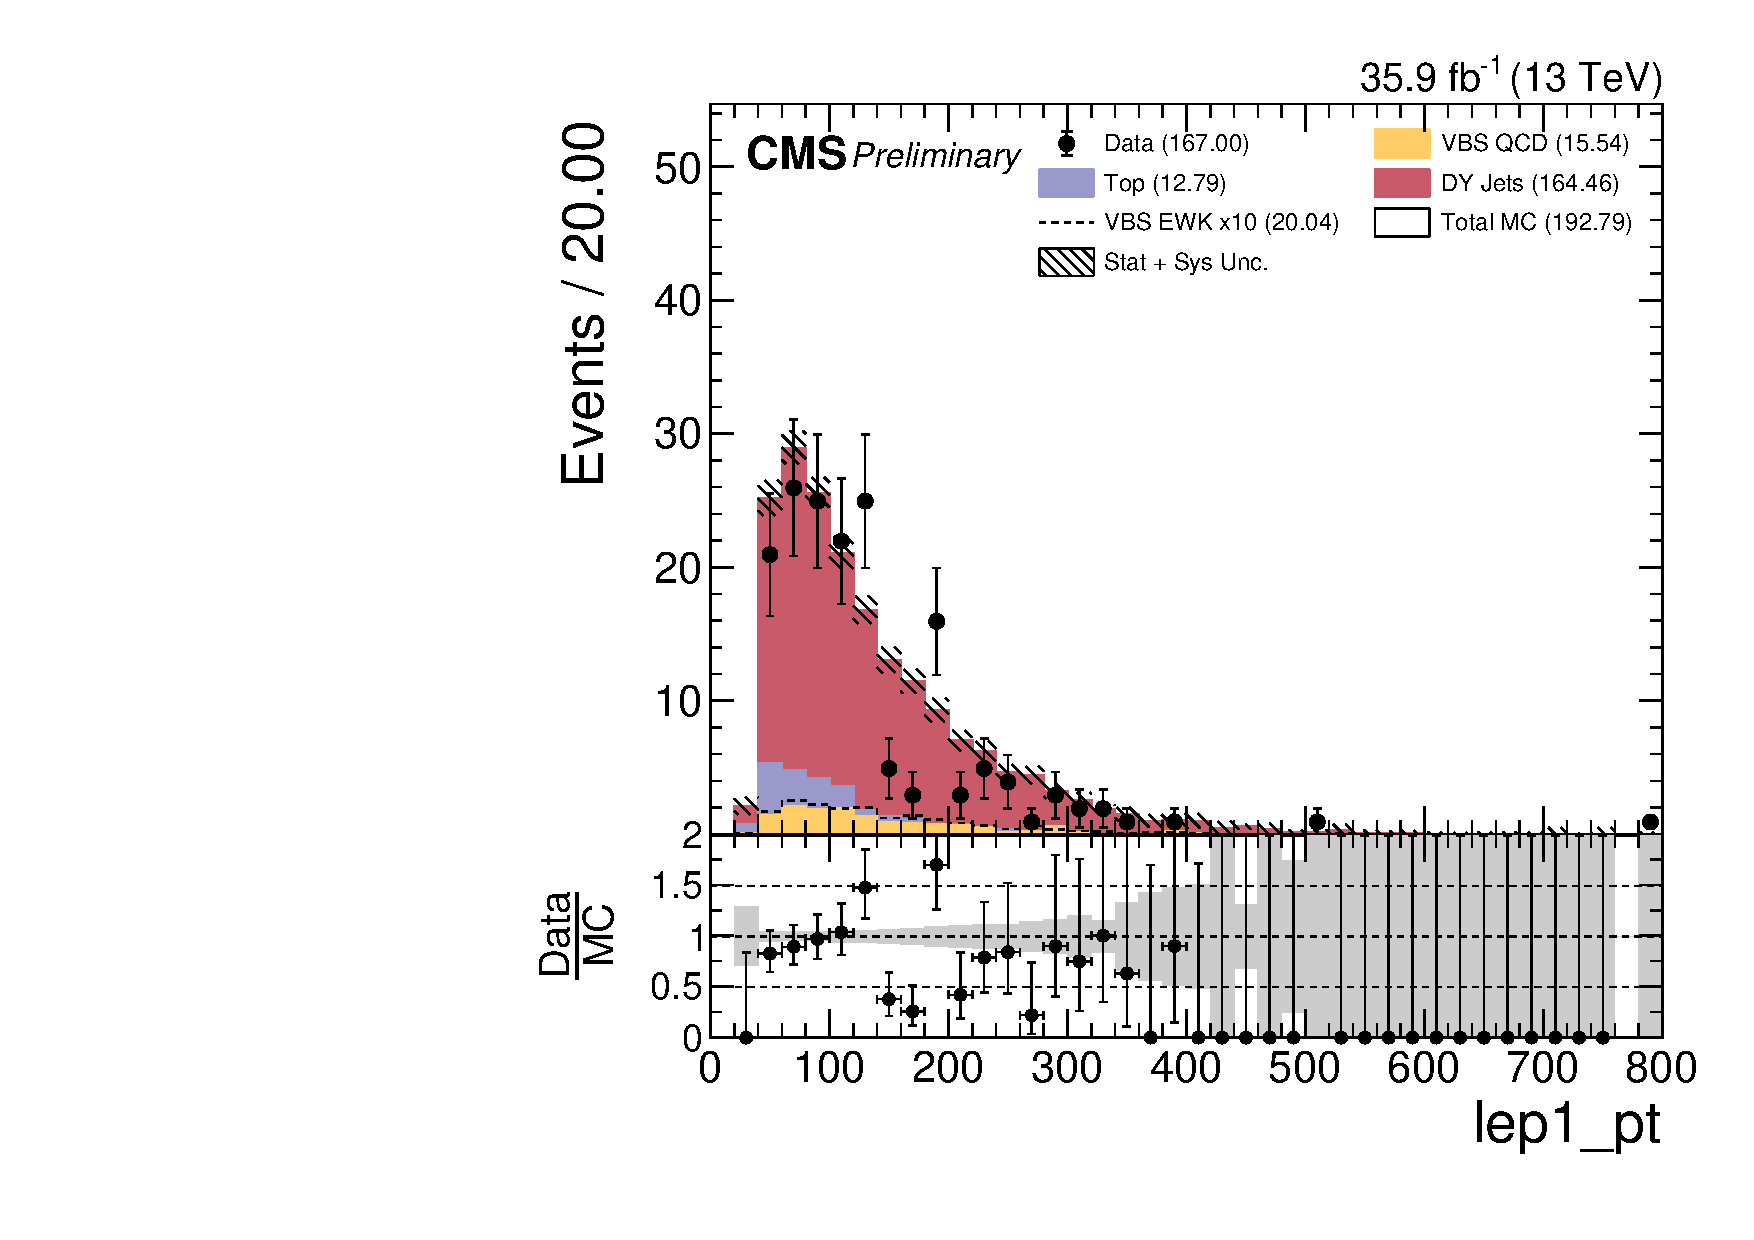
\includegraphics[width=0.30\textwidth]{analysis_plots/2016_zv/cr_vjets_e/lep1_pt.pdf}
  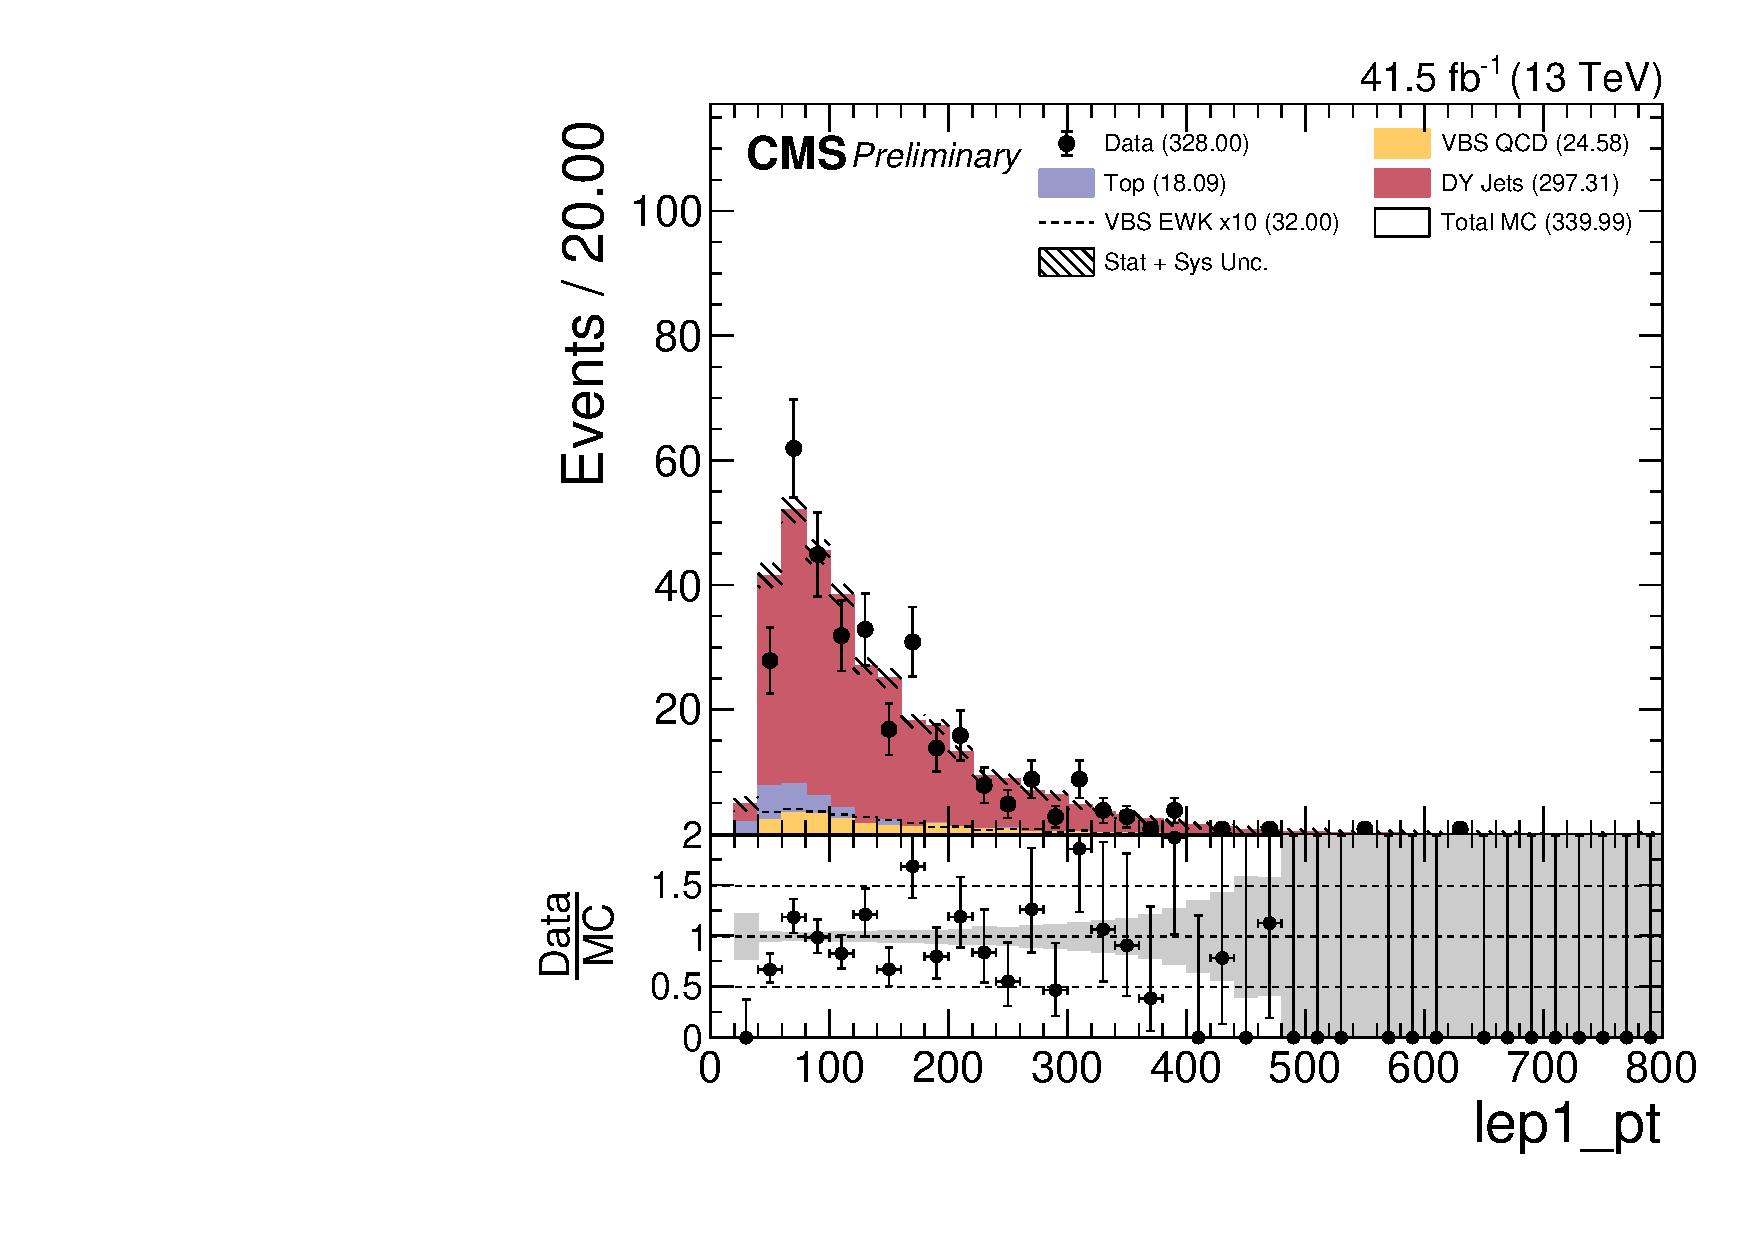
\includegraphics[width=0.30\textwidth]{analysis_plots/2017_zv/cr_vjets_e/lep1_pt.pdf}
  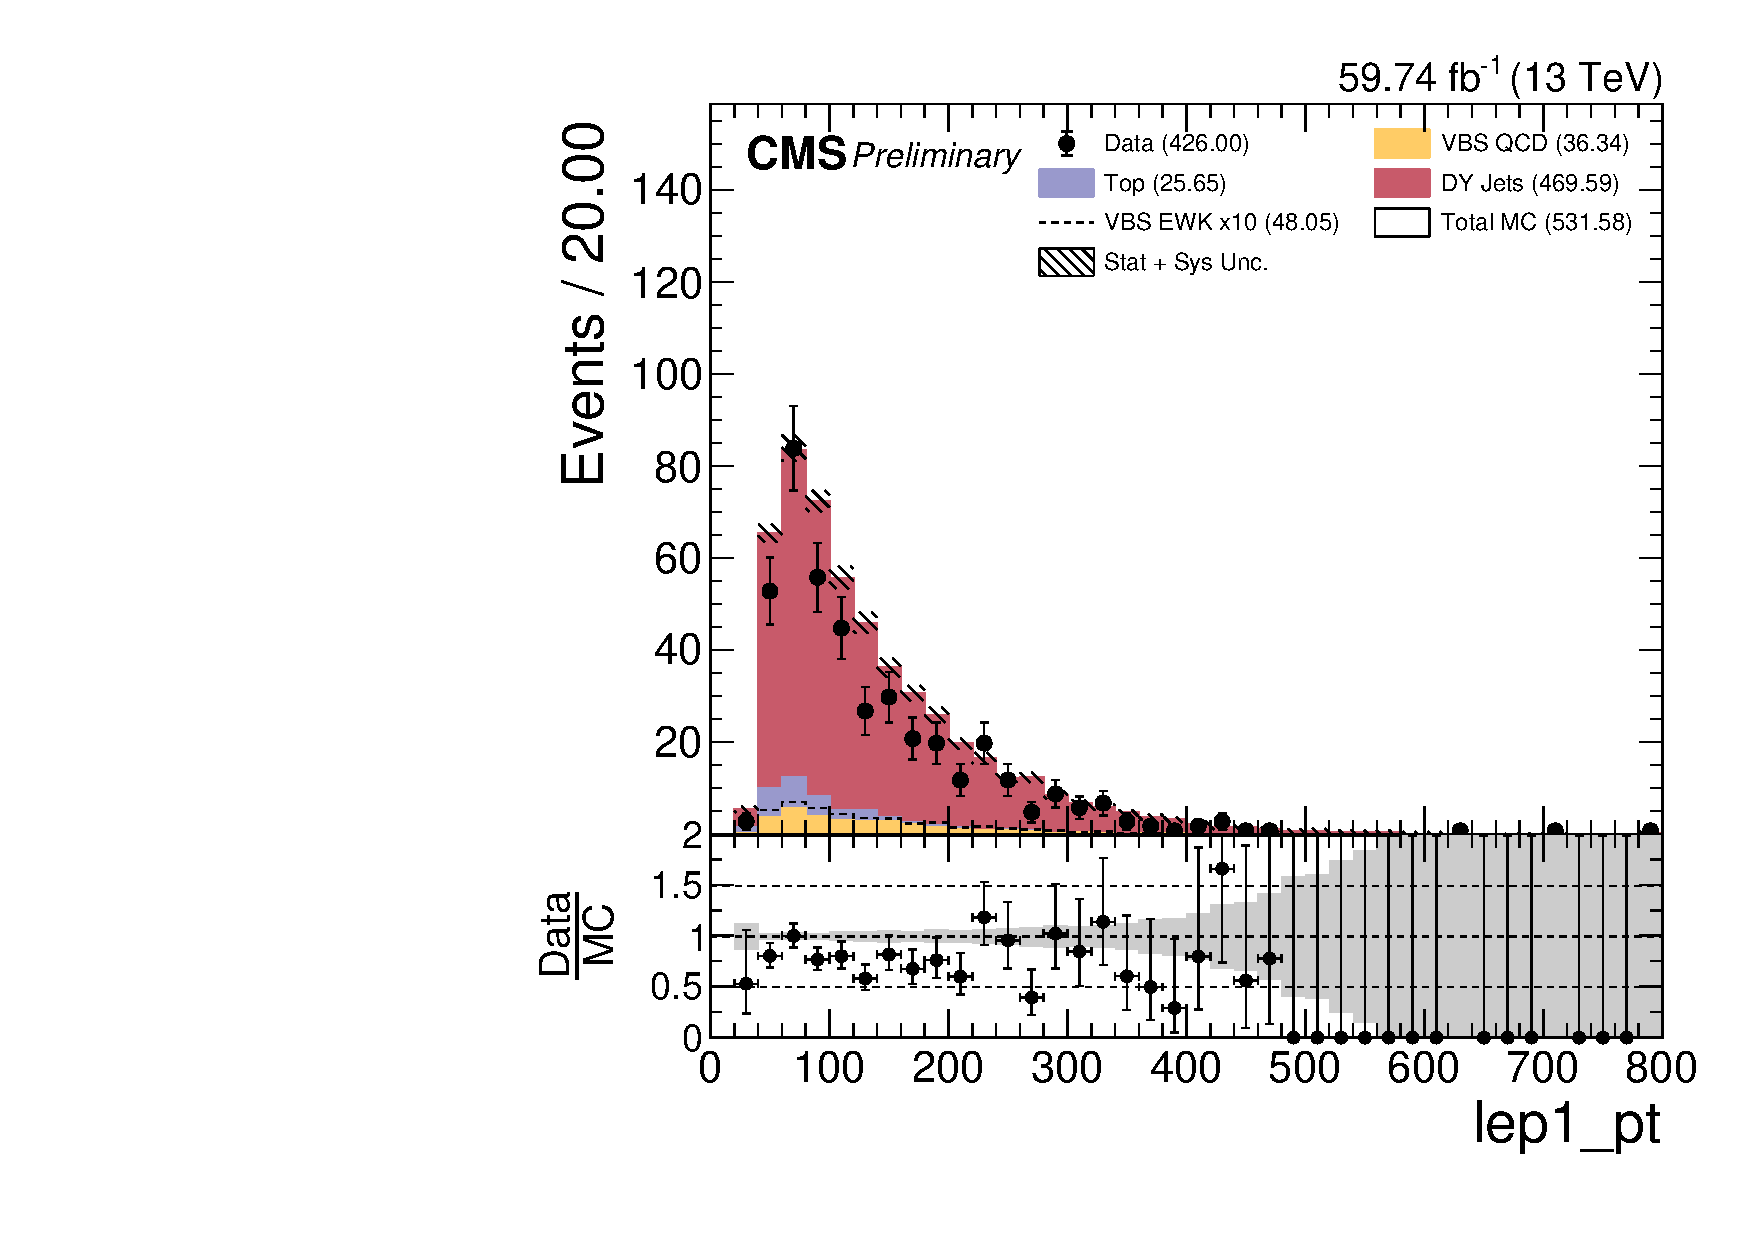
\includegraphics[width=0.30\textwidth]{analysis_plots/2018_zv/cr_vjets_e/lep1_pt.pdf} \\
  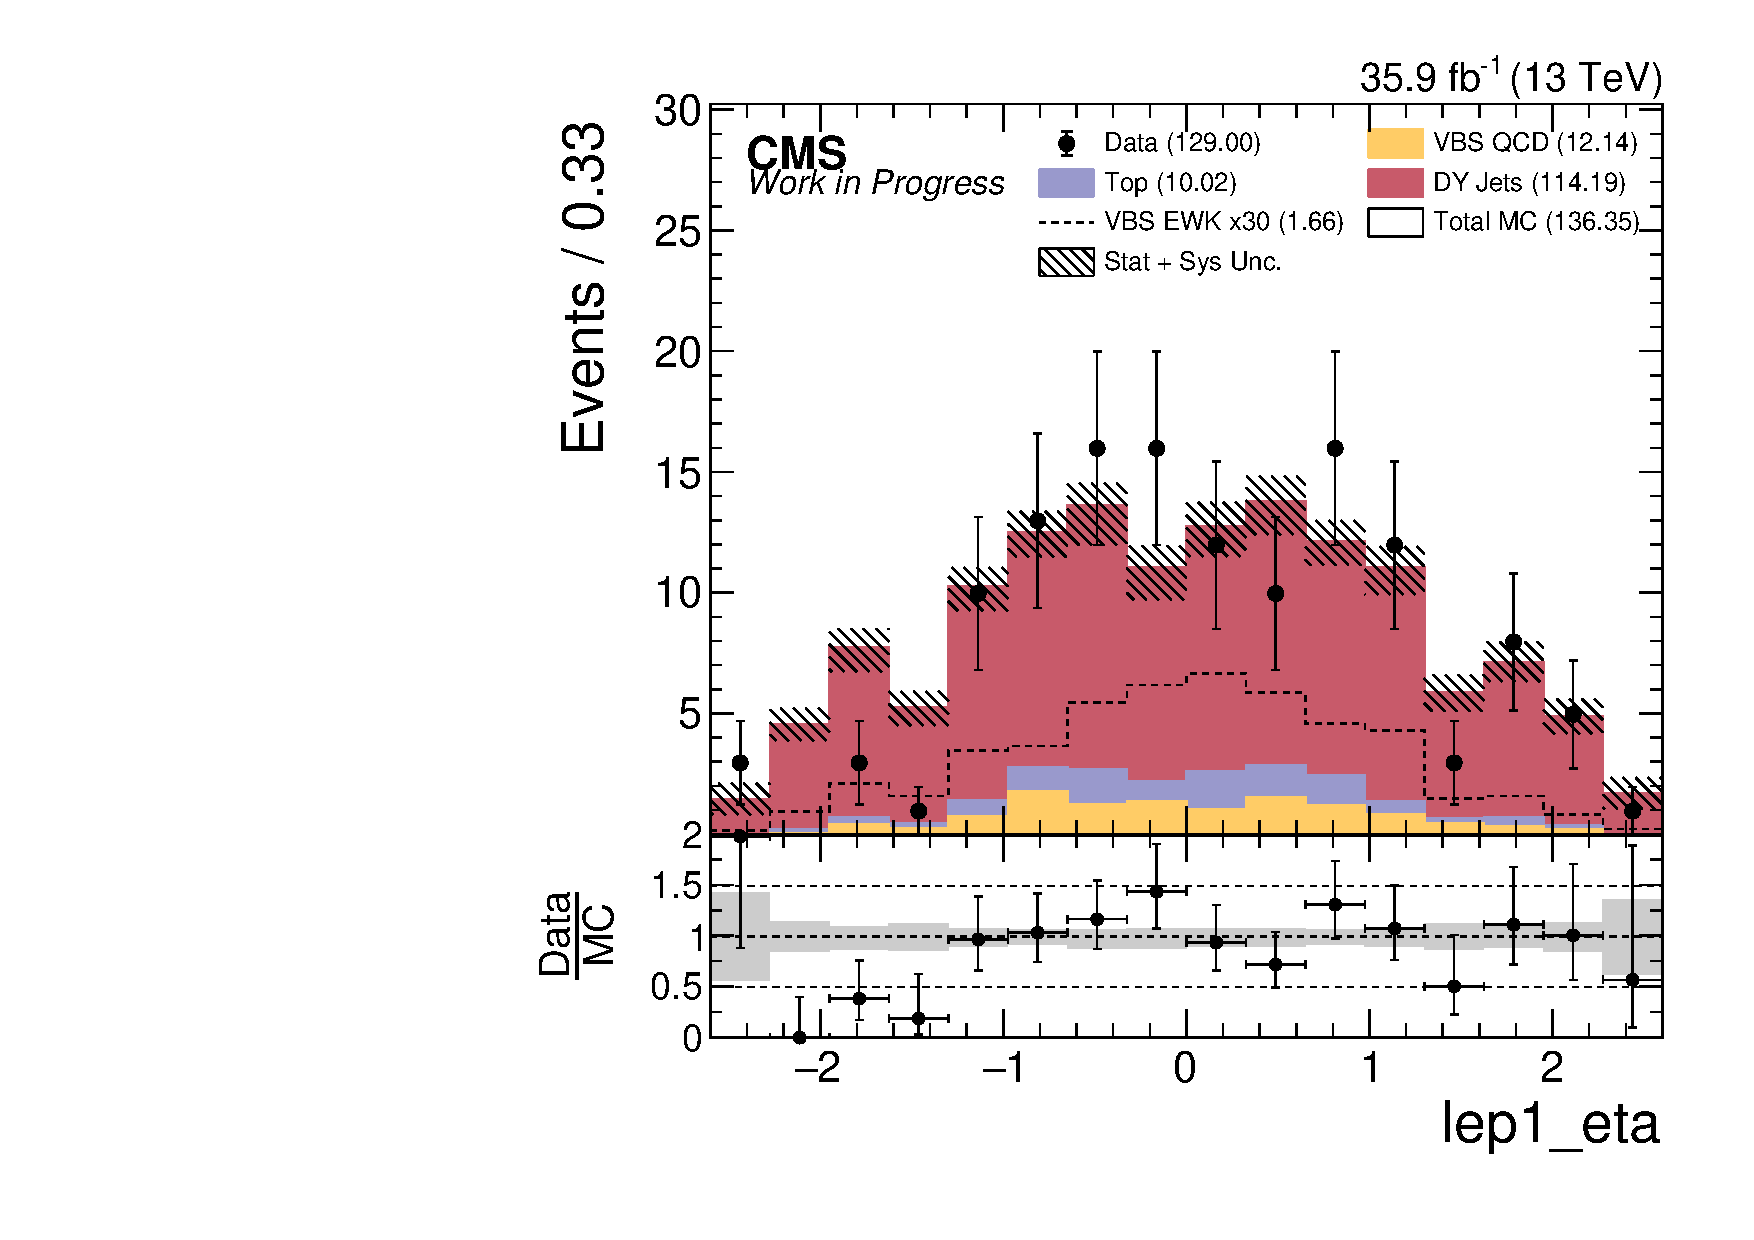
\includegraphics[width=0.30\textwidth]{analysis_plots/2016_zv/cr_vjets_e/lep1_eta.pdf}
  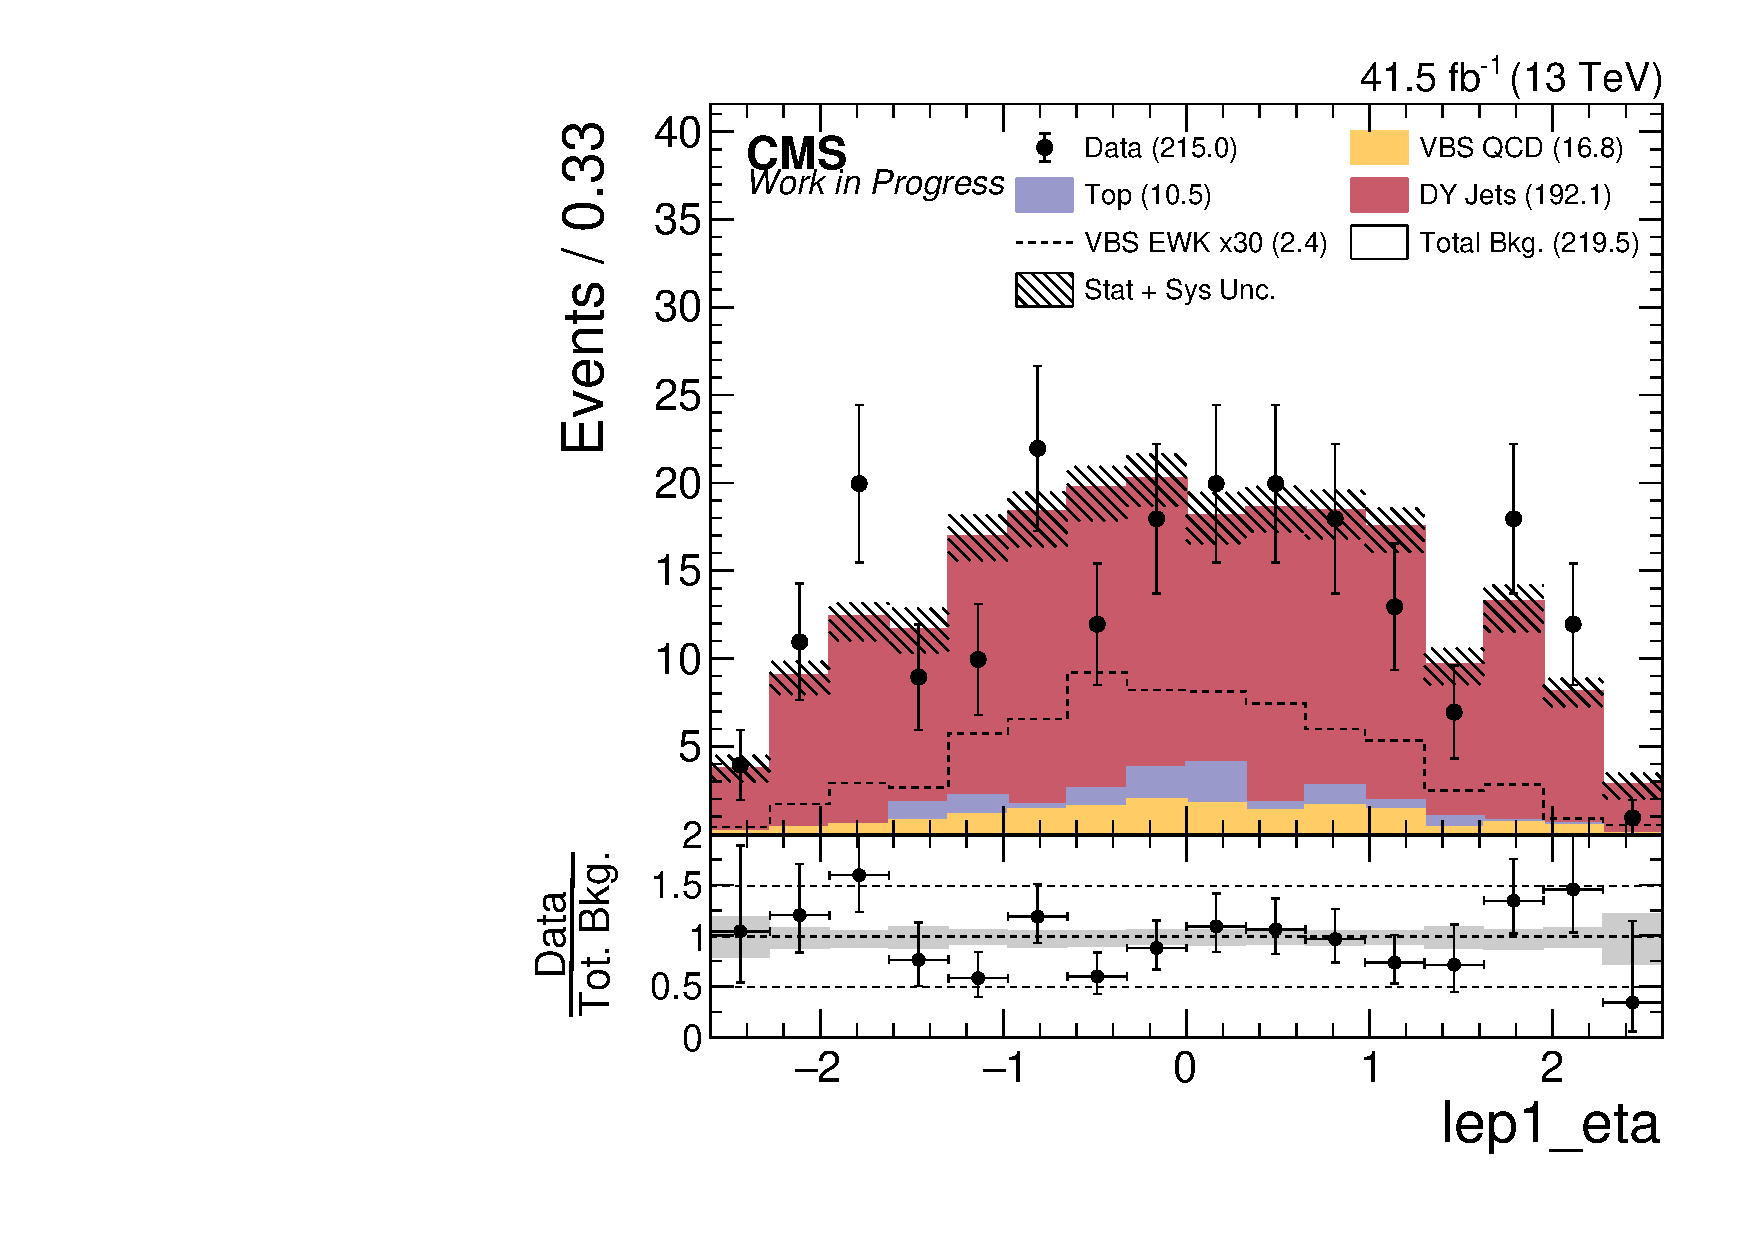
\includegraphics[width=0.30\textwidth]{analysis_plots/2017_zv/cr_vjets_e/lep1_eta.pdf}
  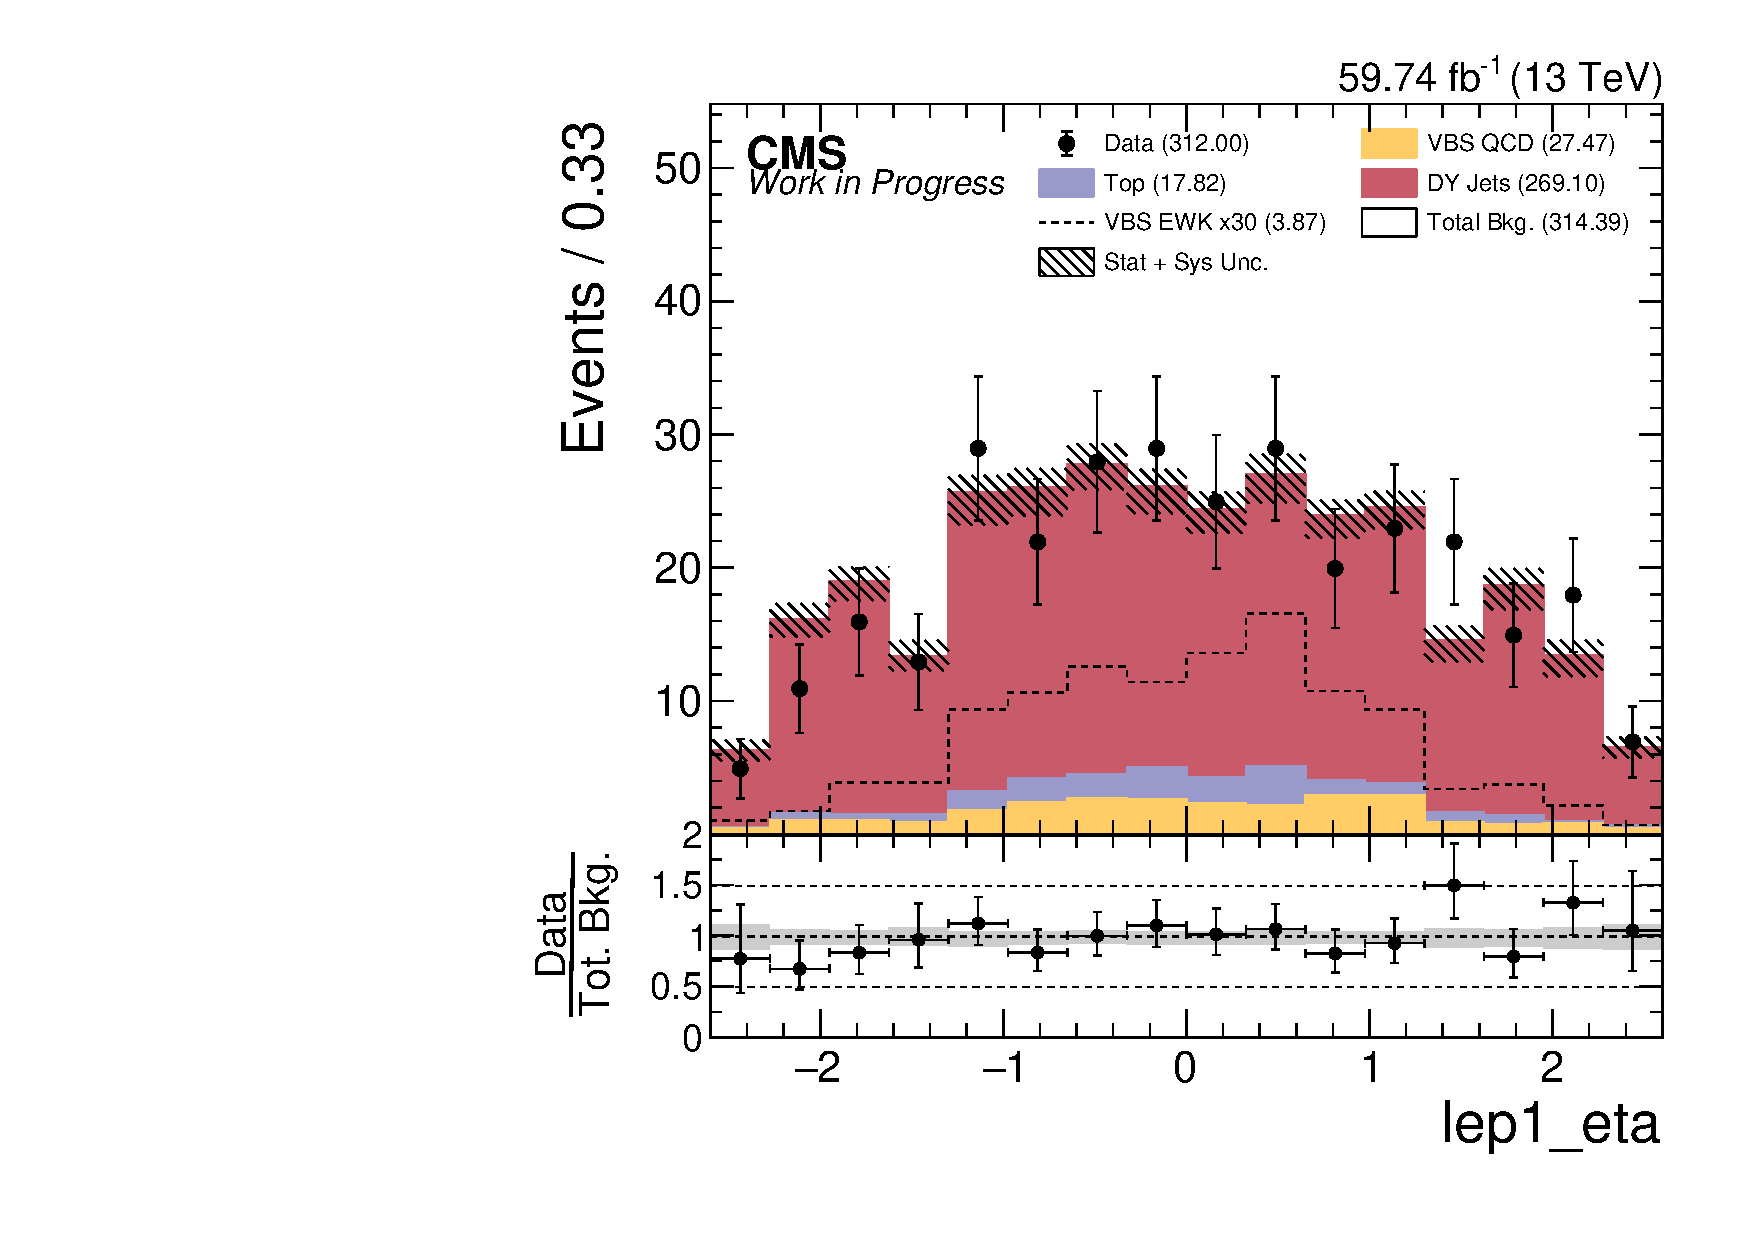
\includegraphics[width=0.30\textwidth]{analysis_plots/2018_zv/cr_vjets_e/lep1_eta.pdf} \\
  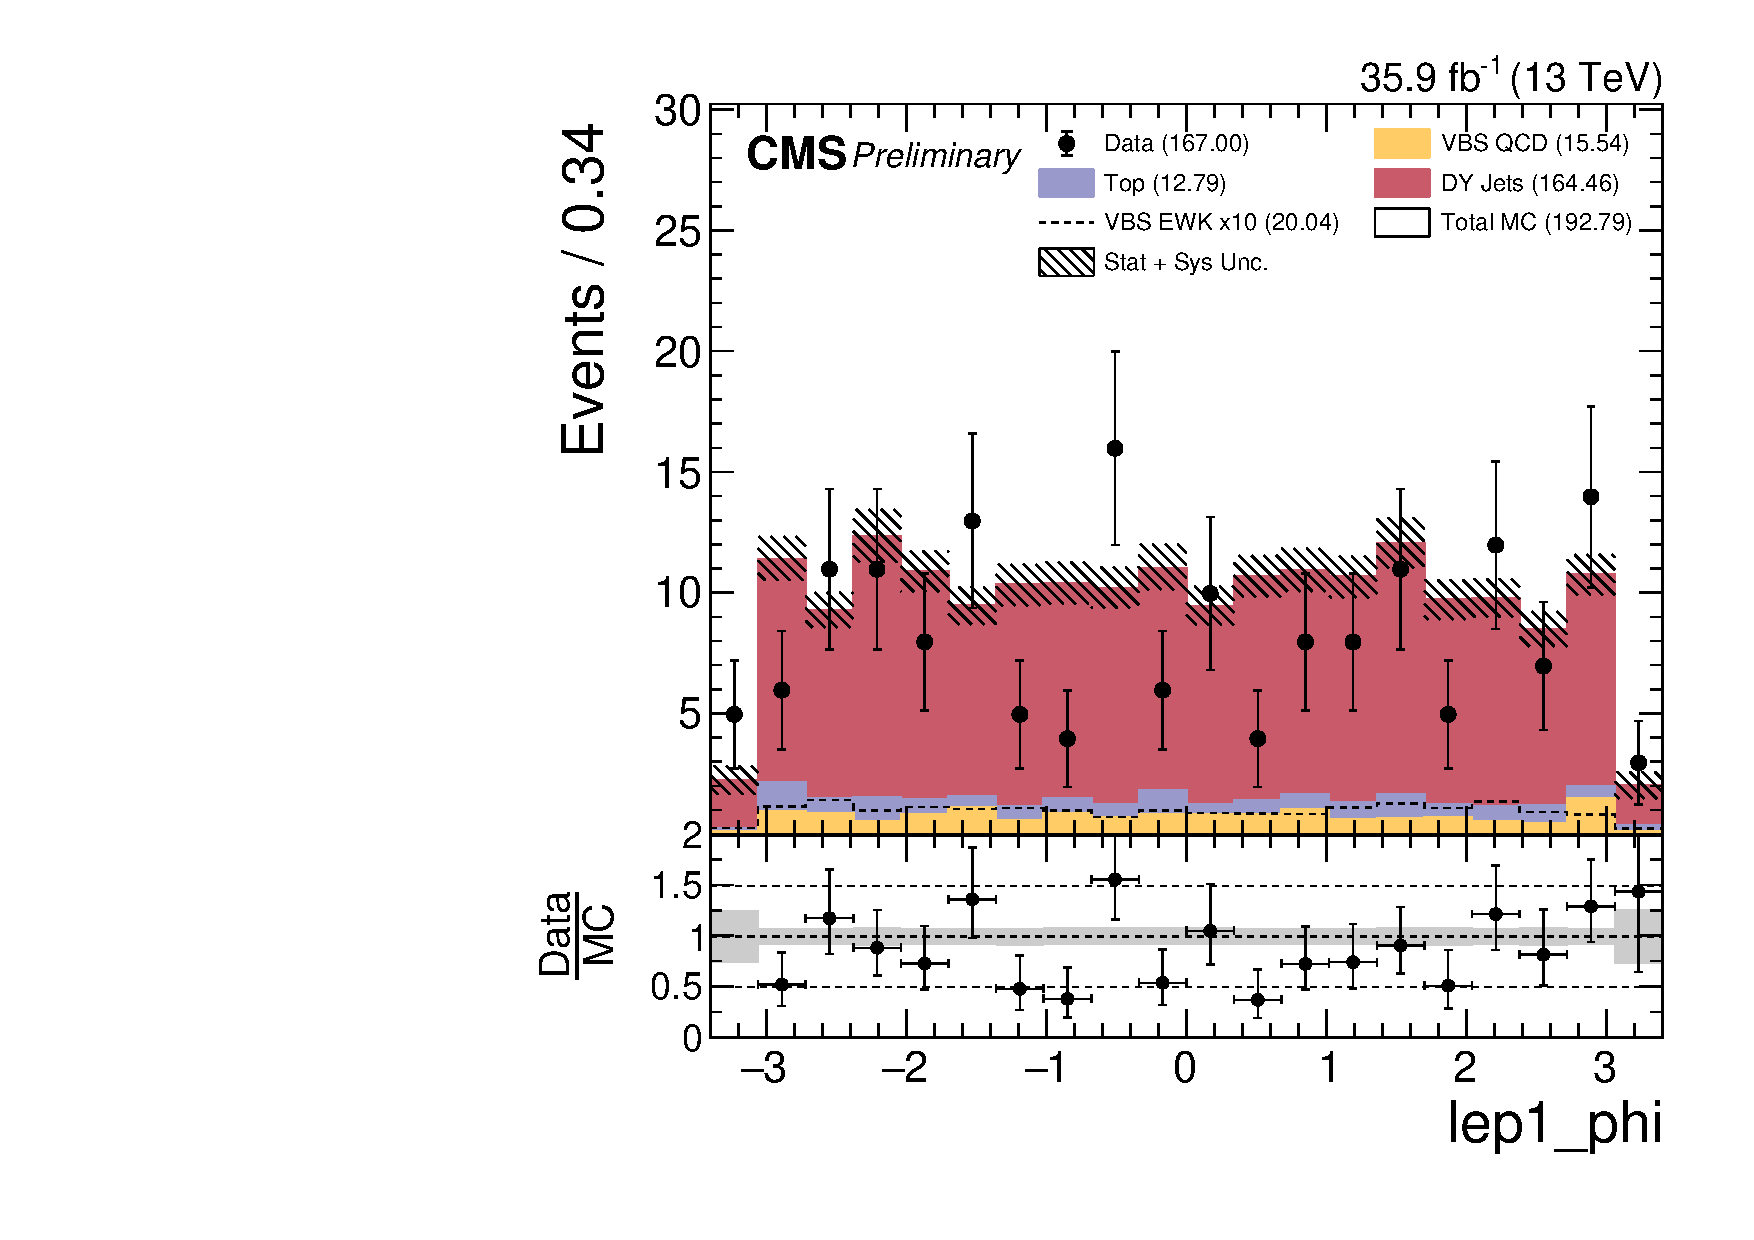
\includegraphics[width=0.30\textwidth]{analysis_plots/2016_zv/cr_vjets_e/lep1_phi.pdf}
  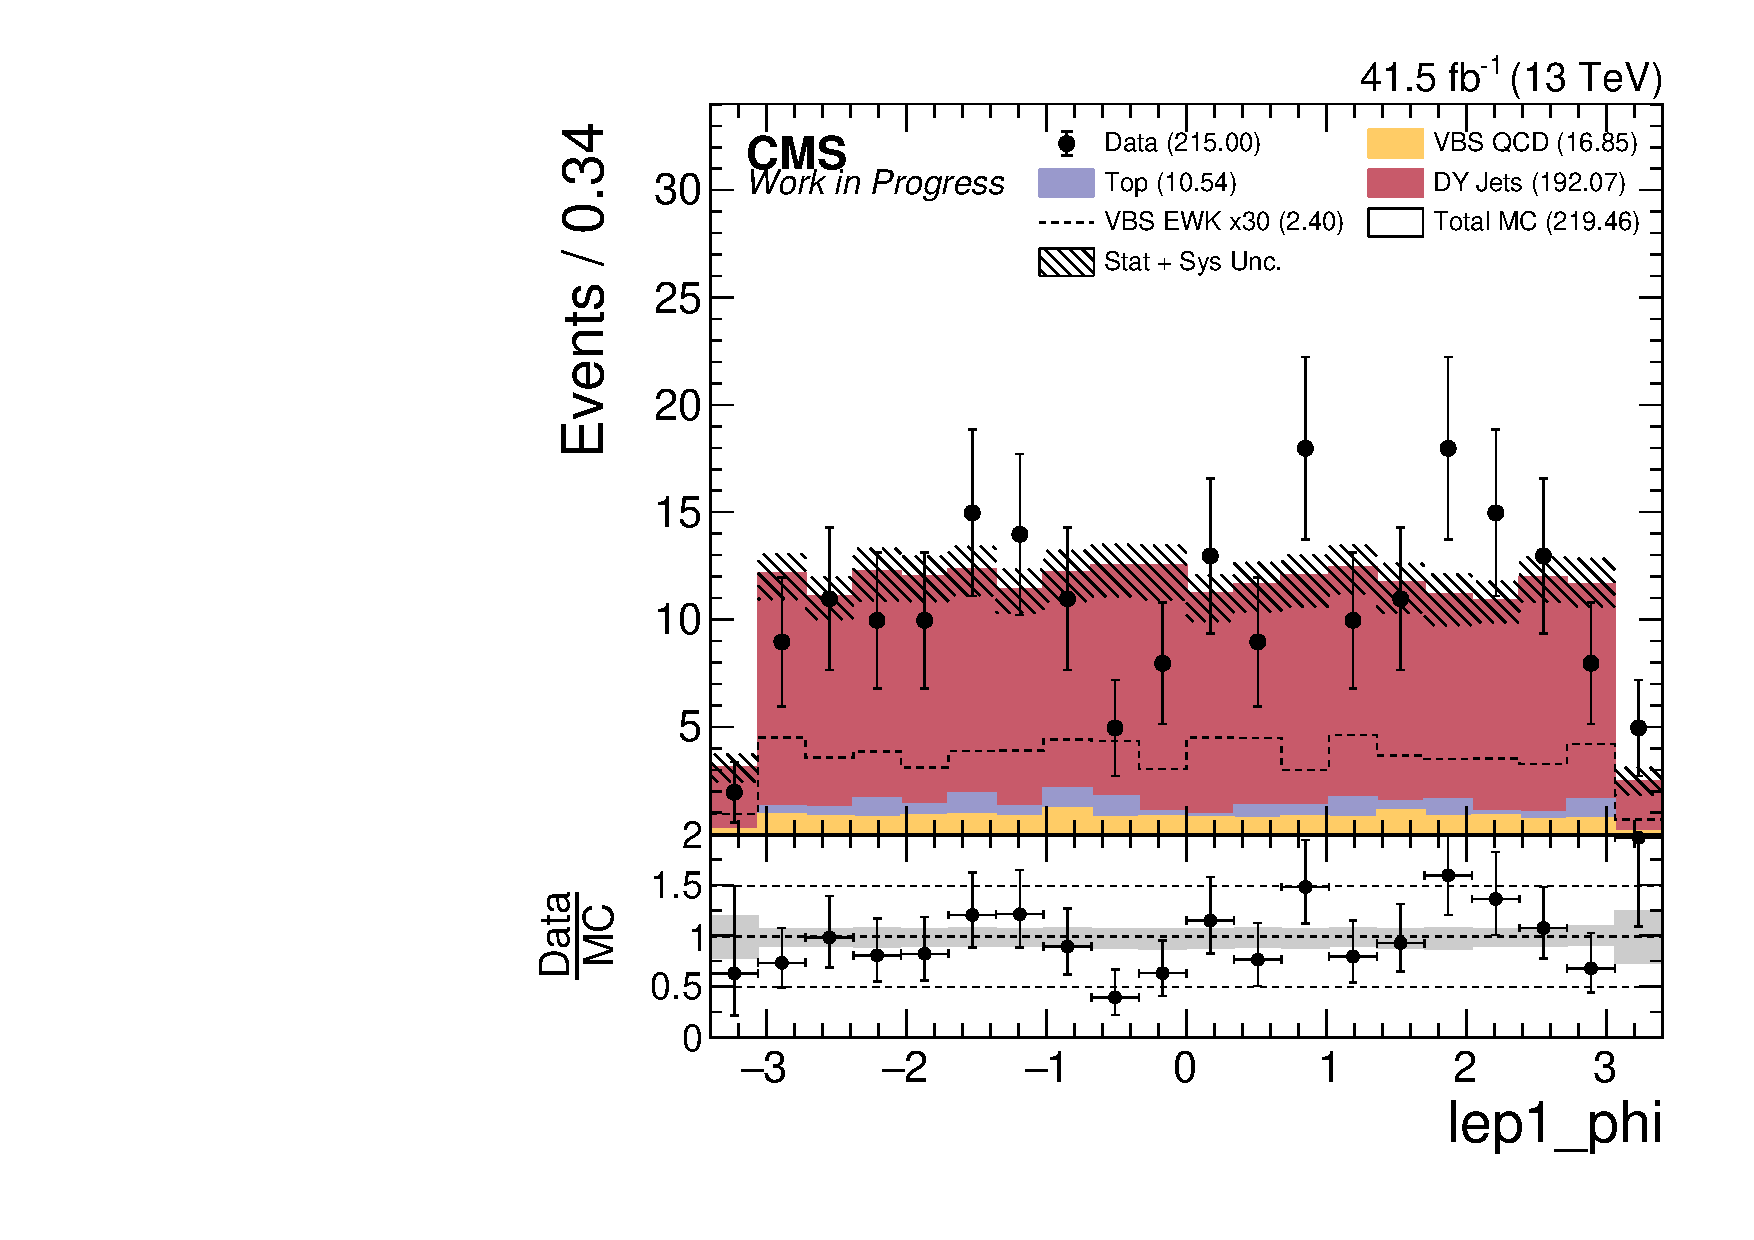
\includegraphics[width=0.30\textwidth]{analysis_plots/2017_zv/cr_vjets_e/lep1_phi.pdf}
  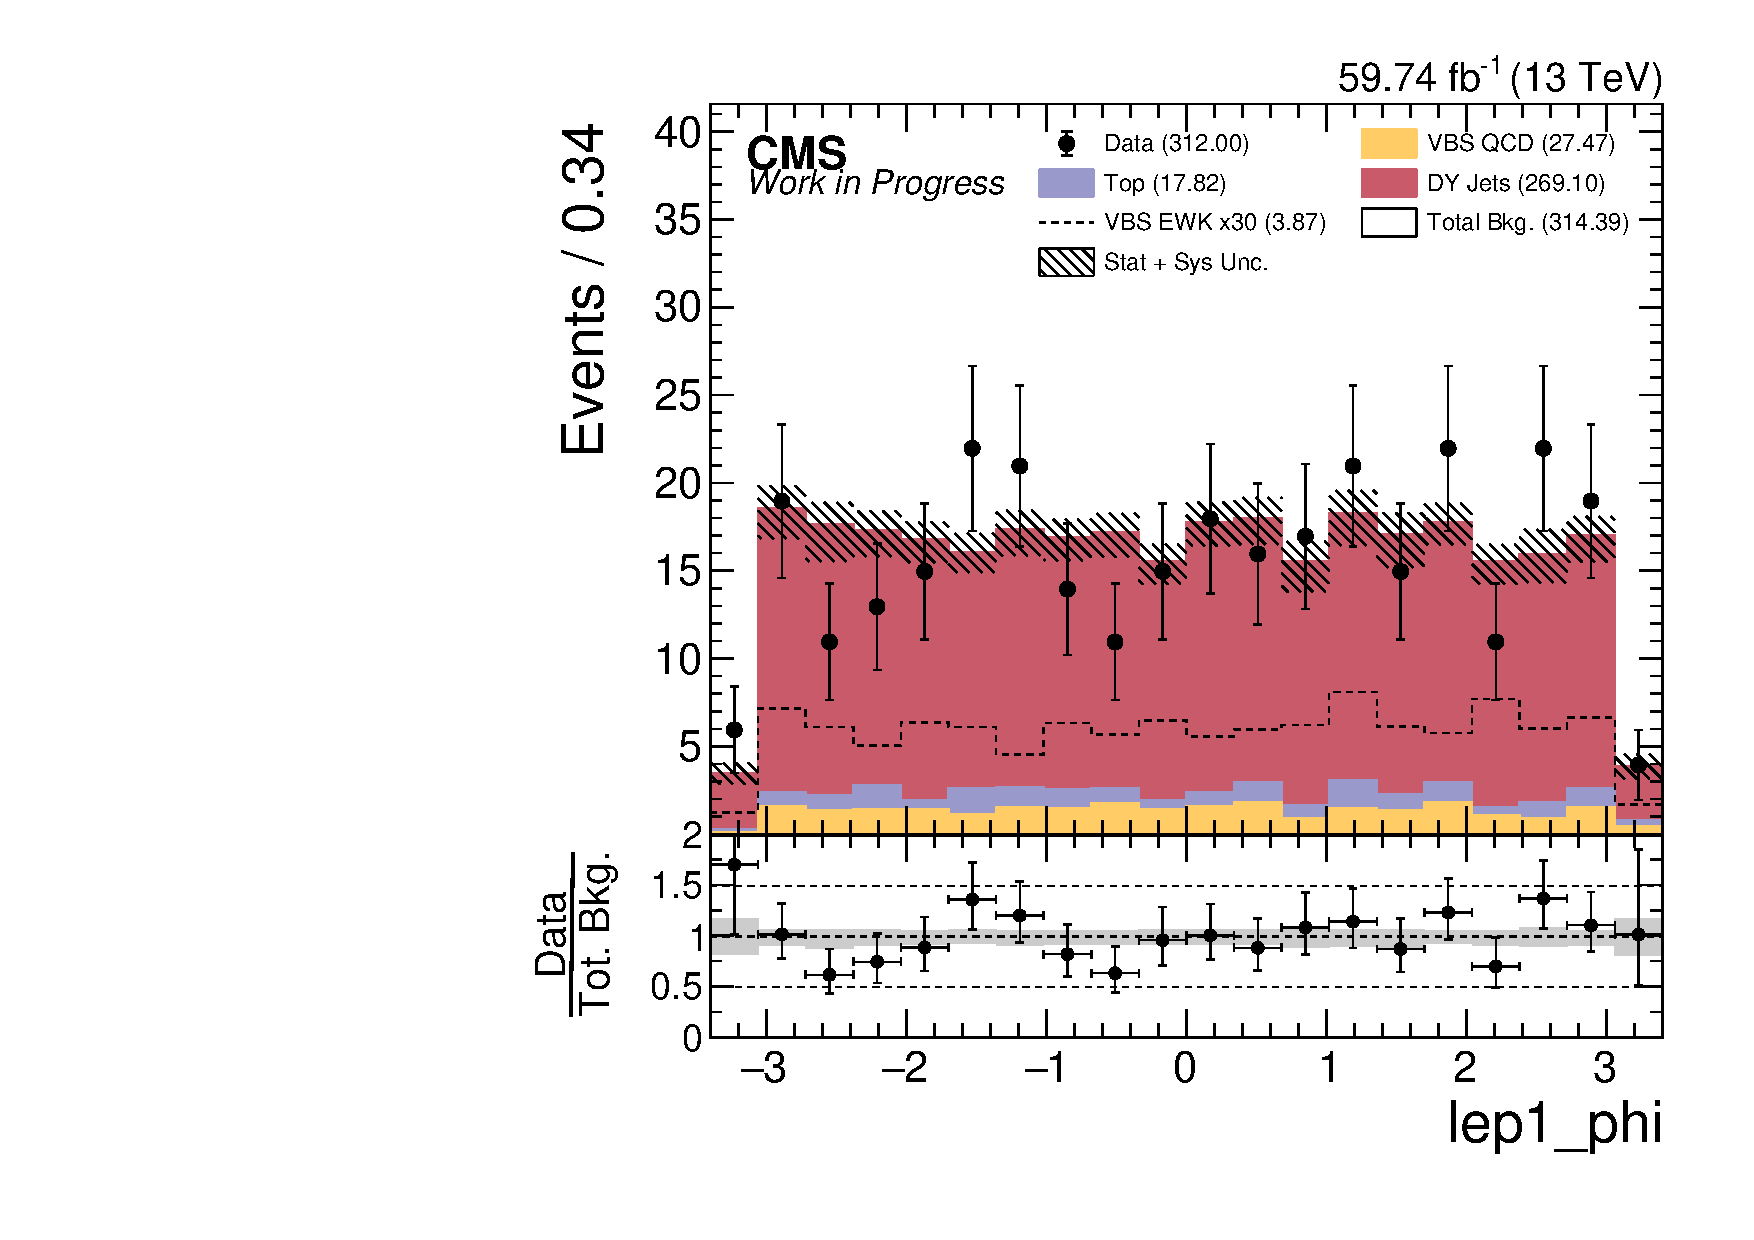
\includegraphics[width=0.30\textwidth]{analysis_plots/2018_zv/cr_vjets_e/lep1_phi.pdf} \\
  \caption[DY+Jets Control Region: Leading electron kinematics in Boosted ZV Channel]%
  {DY+Jets Control Region: Leading electron kinematics in Boosted ZV Channel. From Left to Right: 2016,
    2017, and 2018. From Top to Bottom: \( p_T \), \( \eta \), \( \phi \).}%
  \label{fig:zv-cr-vjets-e-lep1-pt-eta-phi}
\end{figure}

\begin{figure}[!ht]
  \centering
  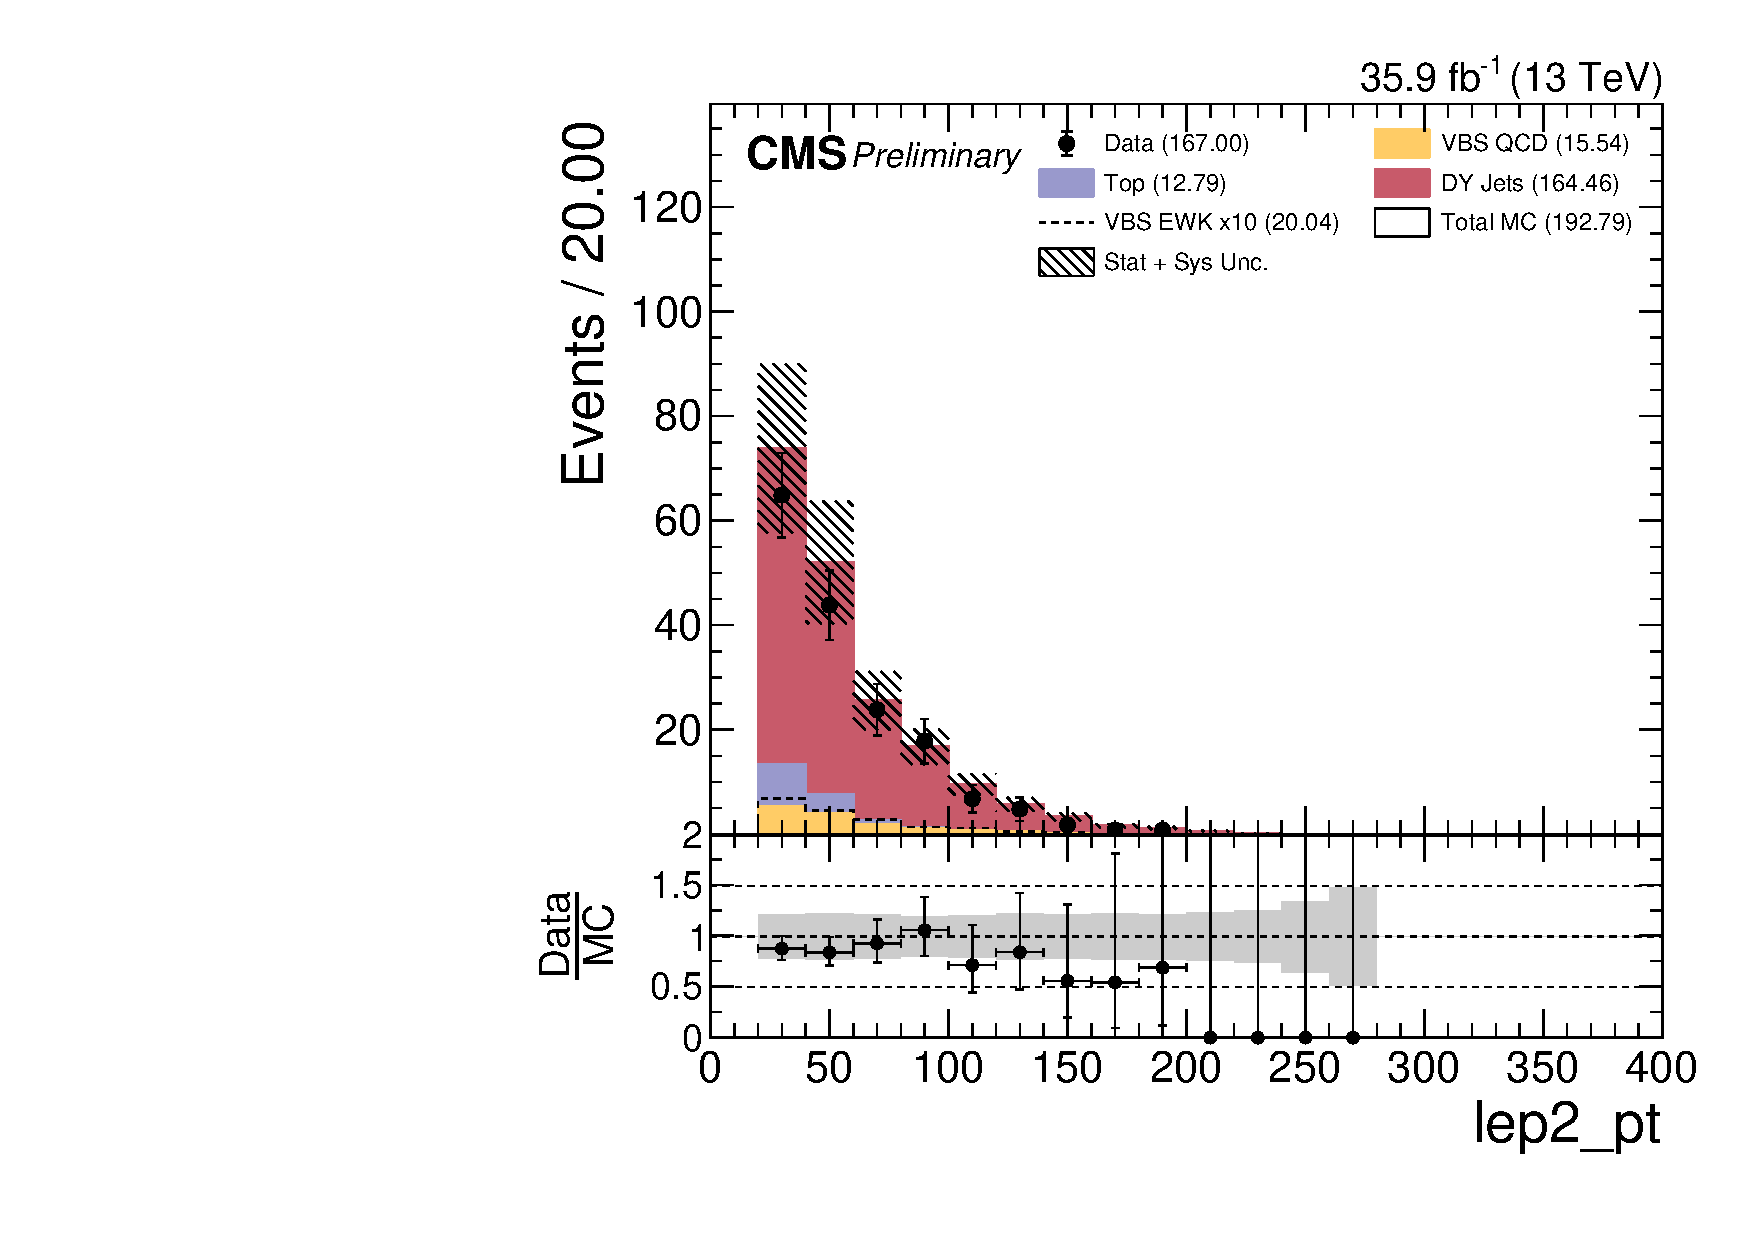
\includegraphics[width=0.30\textwidth]{analysis_plots/2016_zv/cr_vjets_e/lep2_pt.pdf}
  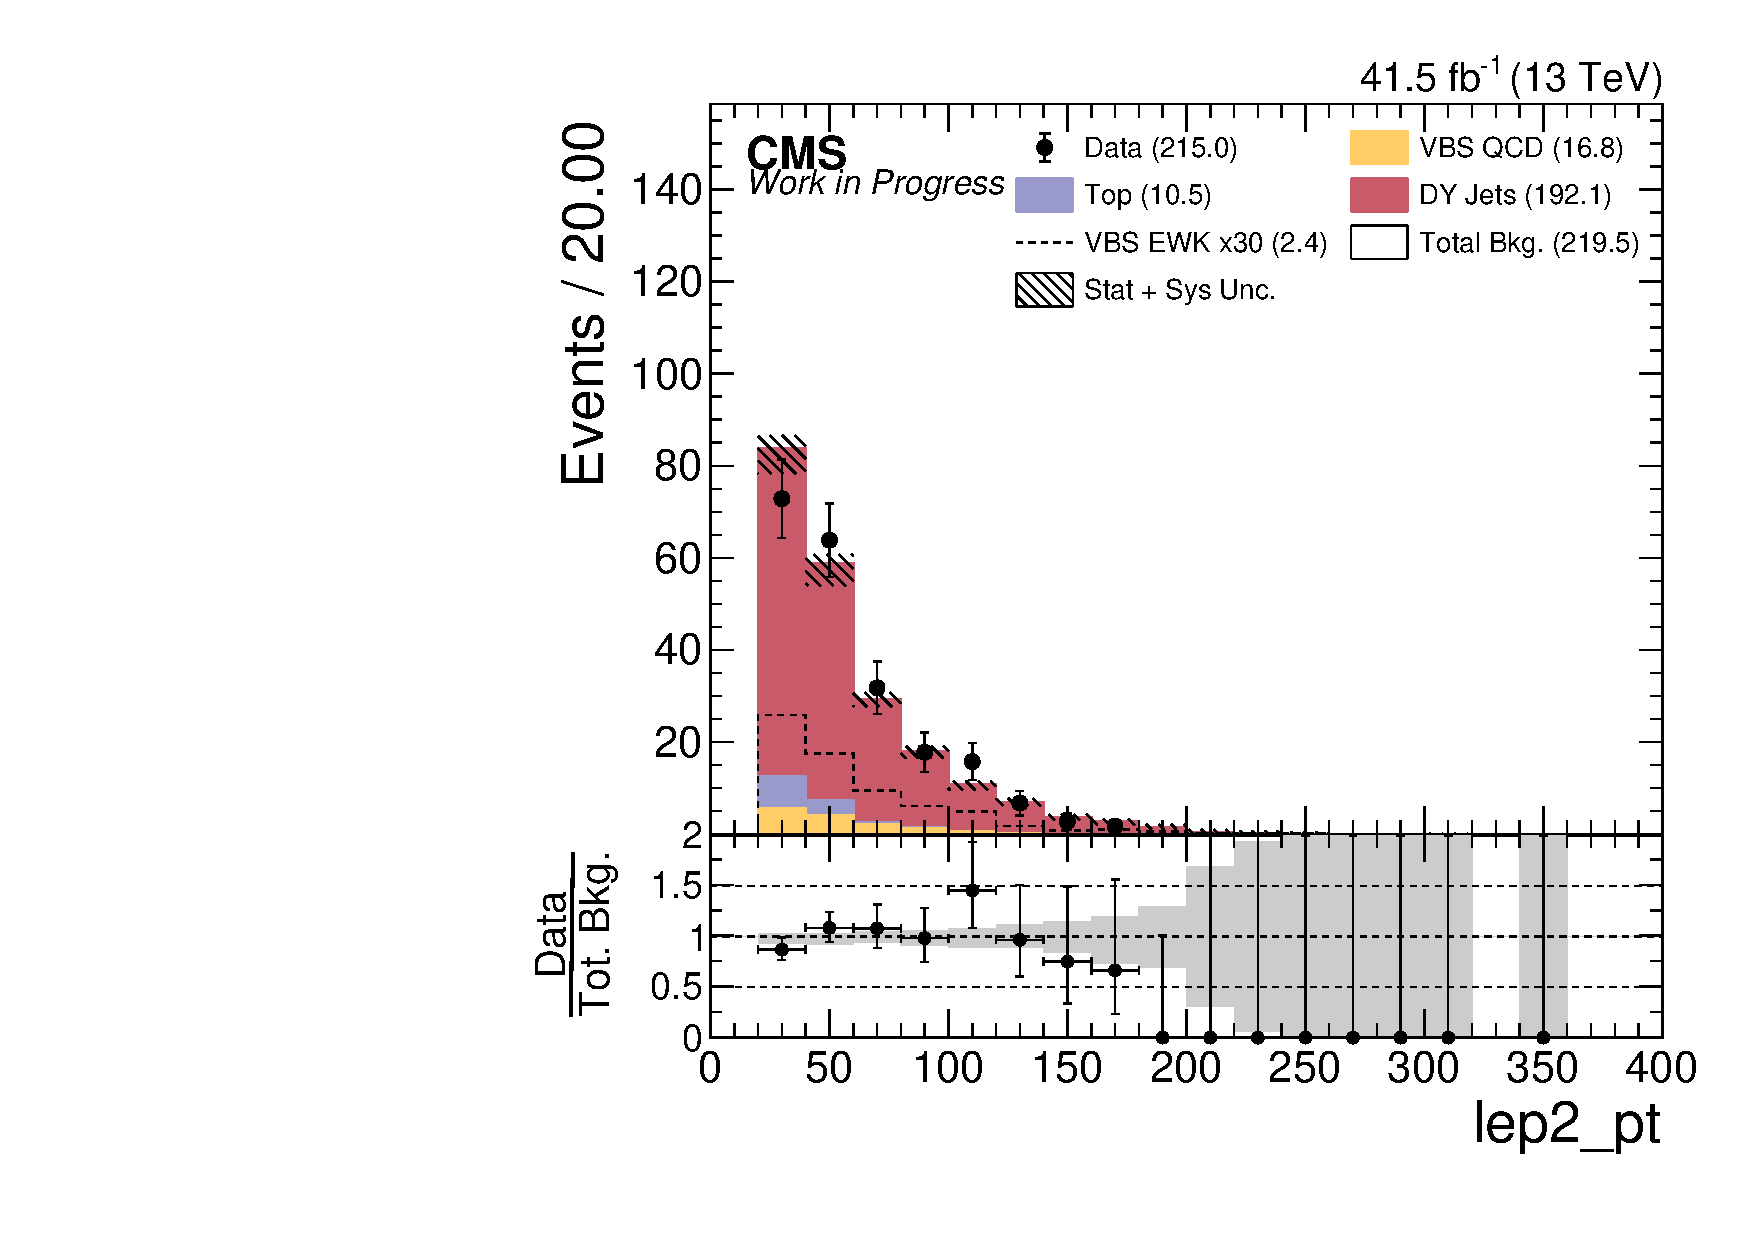
\includegraphics[width=0.30\textwidth]{analysis_plots/2017_zv/cr_vjets_e/lep2_pt.pdf}
  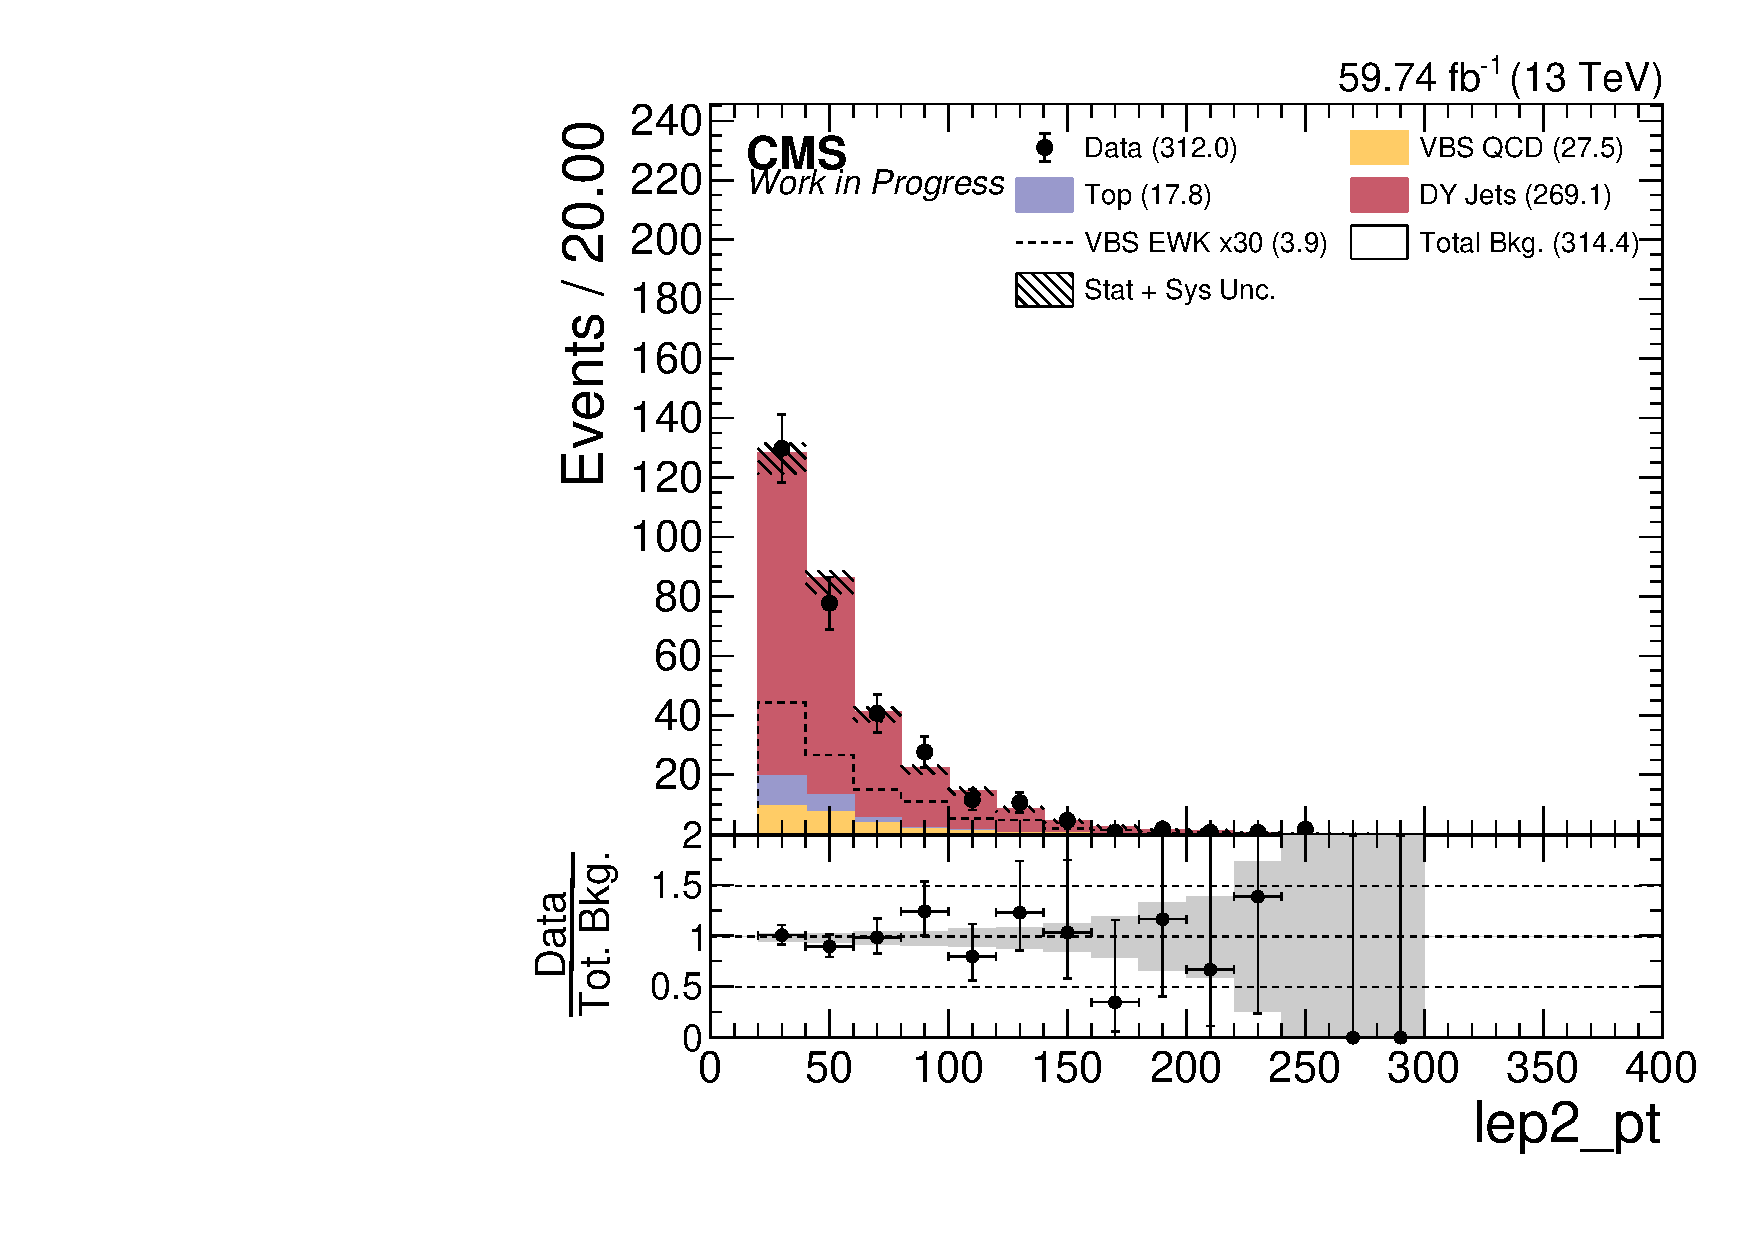
\includegraphics[width=0.30\textwidth]{analysis_plots/2018_zv/cr_vjets_e/lep2_pt.pdf} \\
  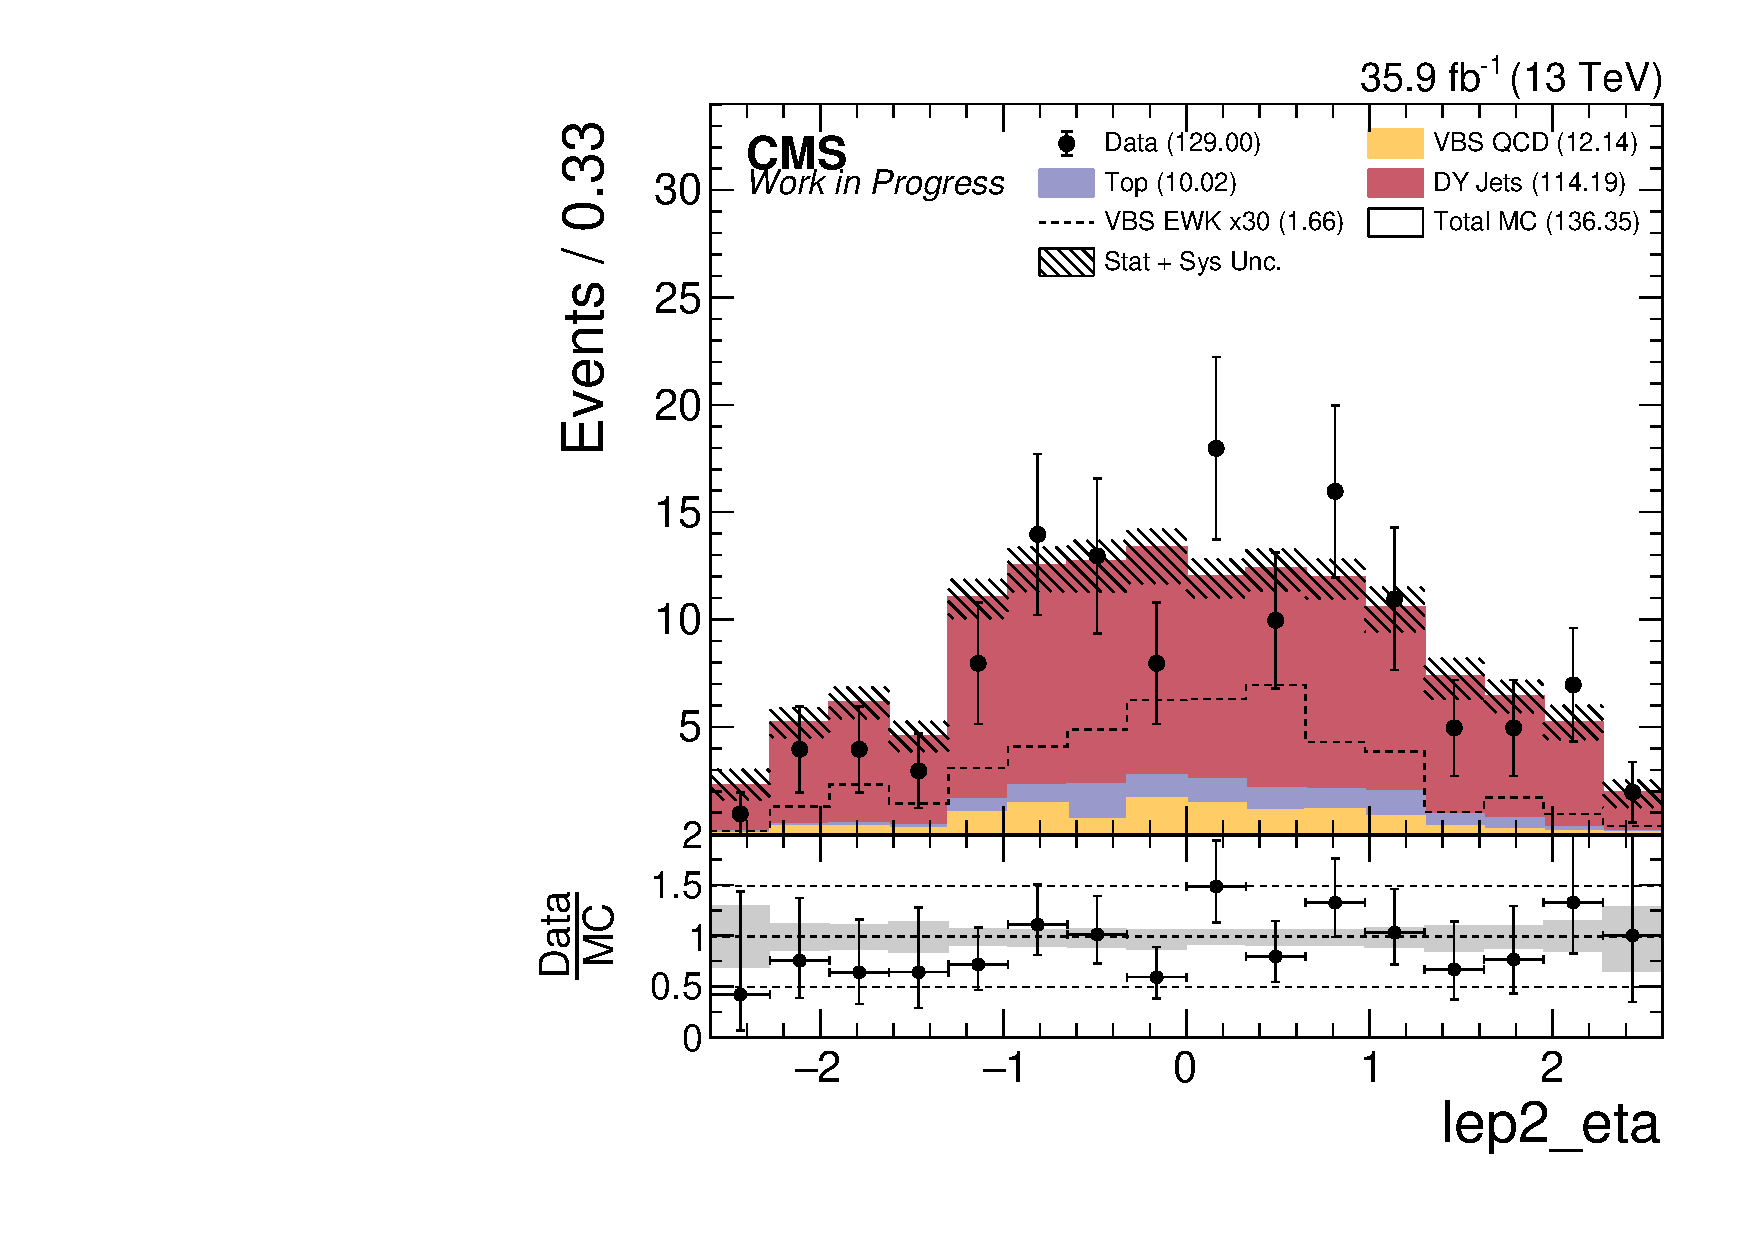
\includegraphics[width=0.30\textwidth]{analysis_plots/2016_zv/cr_vjets_e/lep2_eta.pdf}
  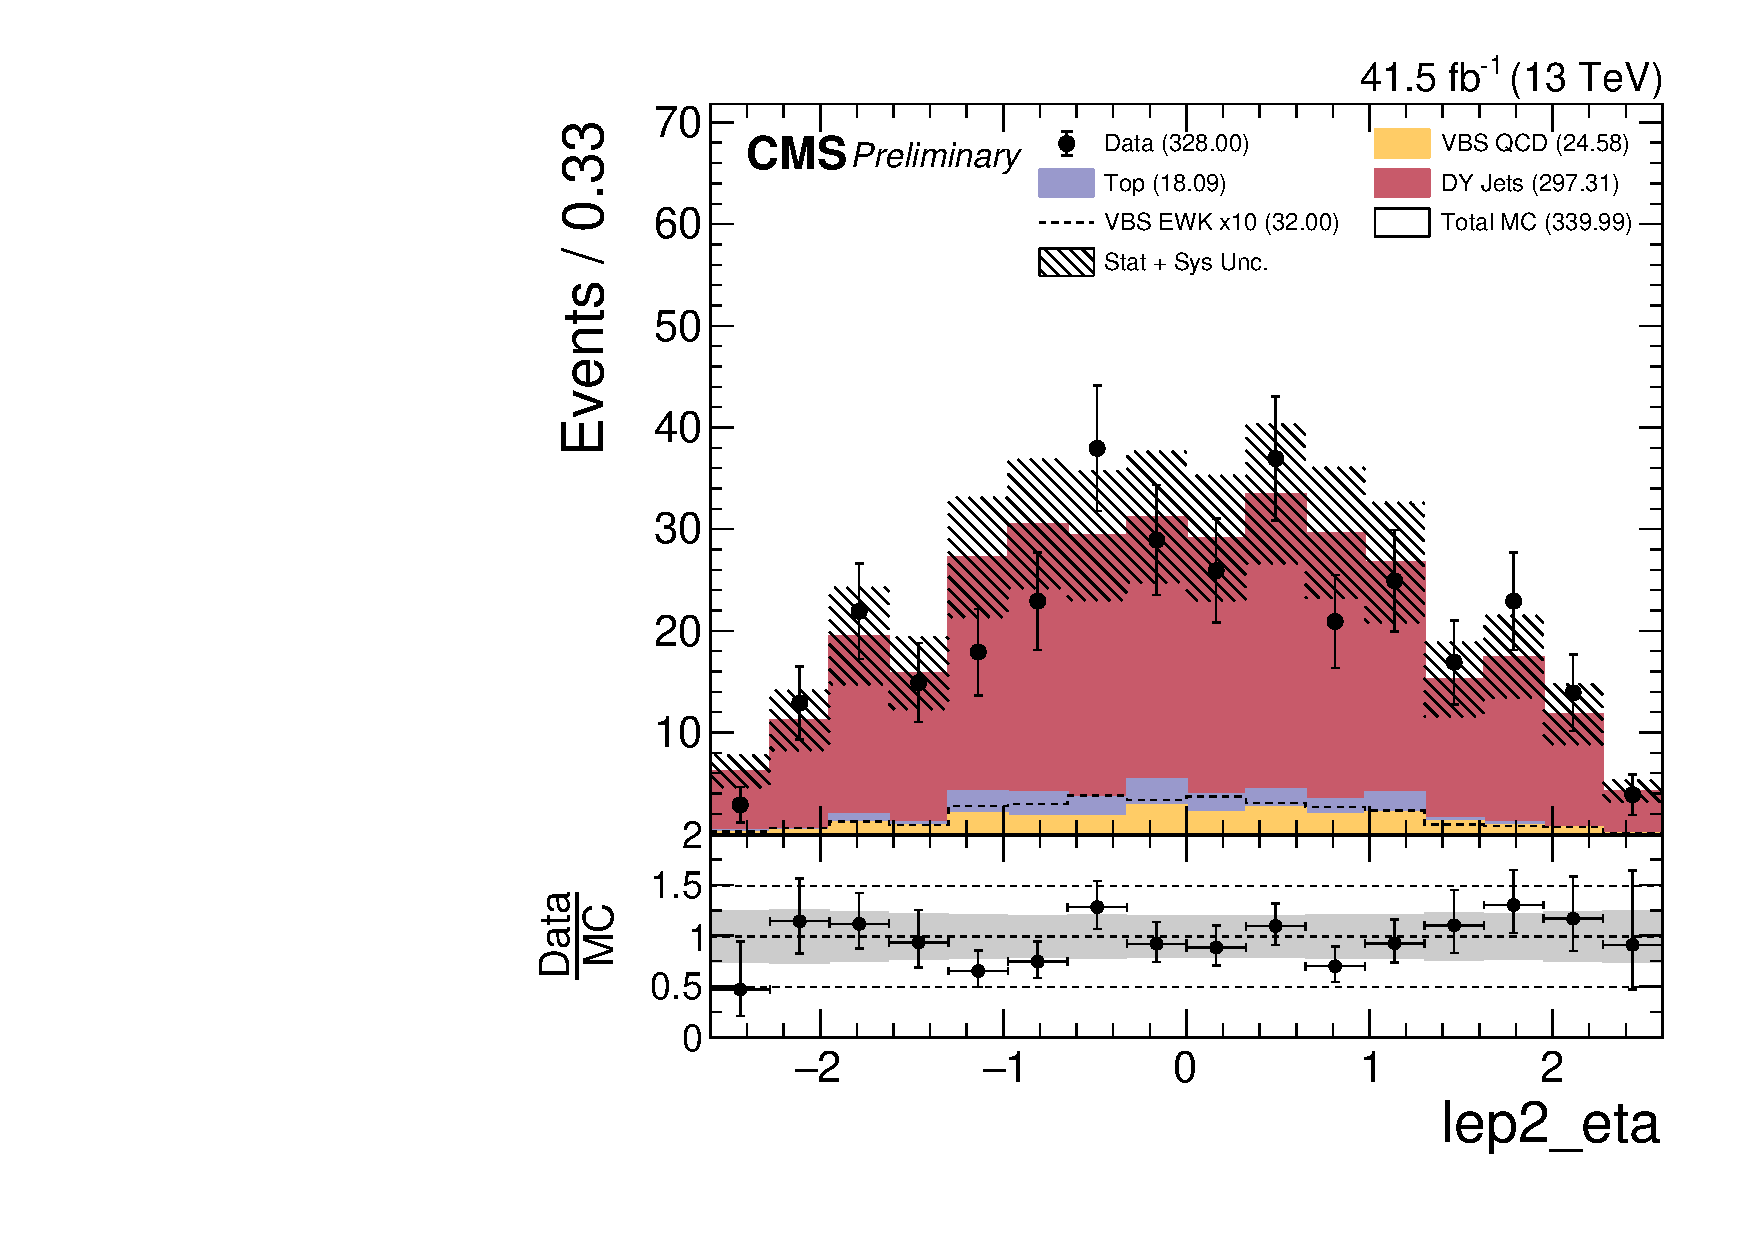
\includegraphics[width=0.30\textwidth]{analysis_plots/2017_zv/cr_vjets_e/lep2_eta.pdf}
  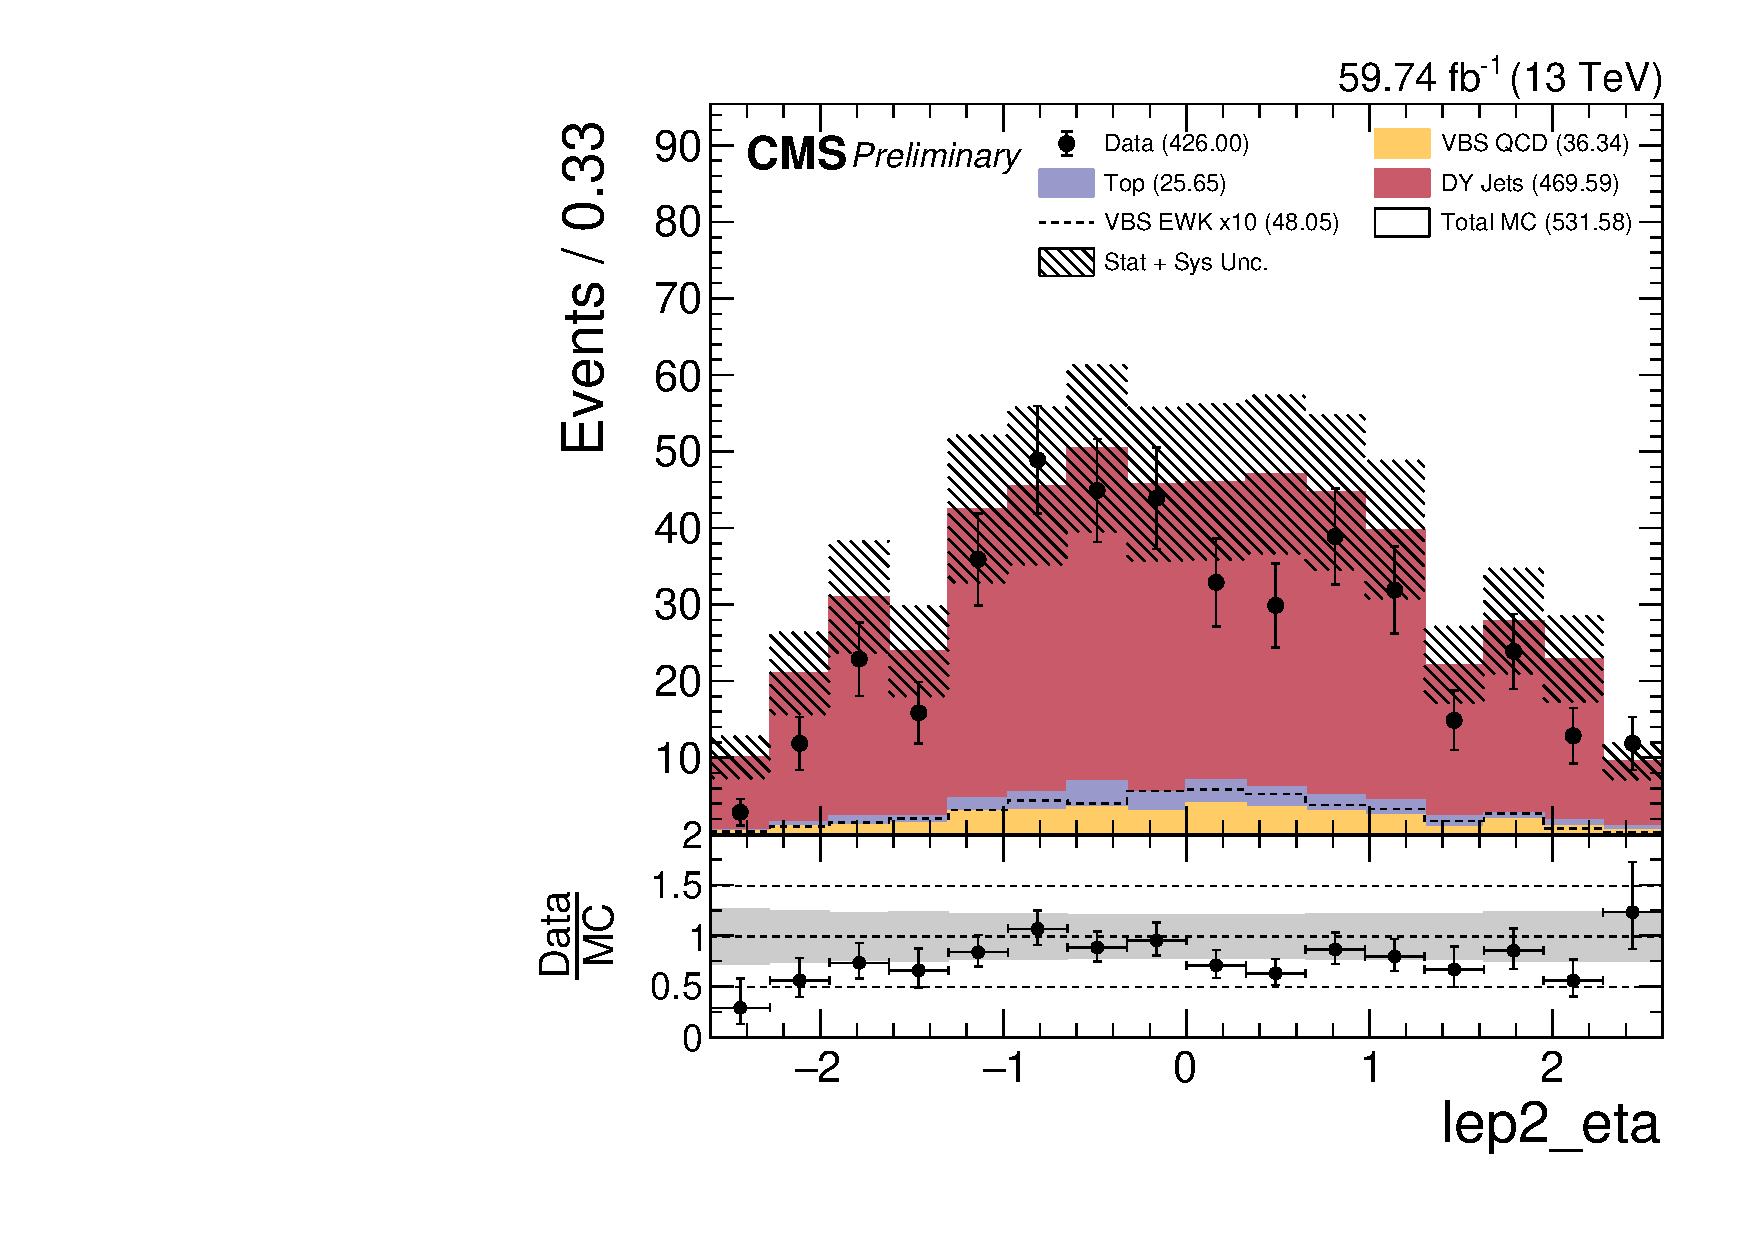
\includegraphics[width=0.30\textwidth]{analysis_plots/2018_zv/cr_vjets_e/lep2_eta.pdf} \\
  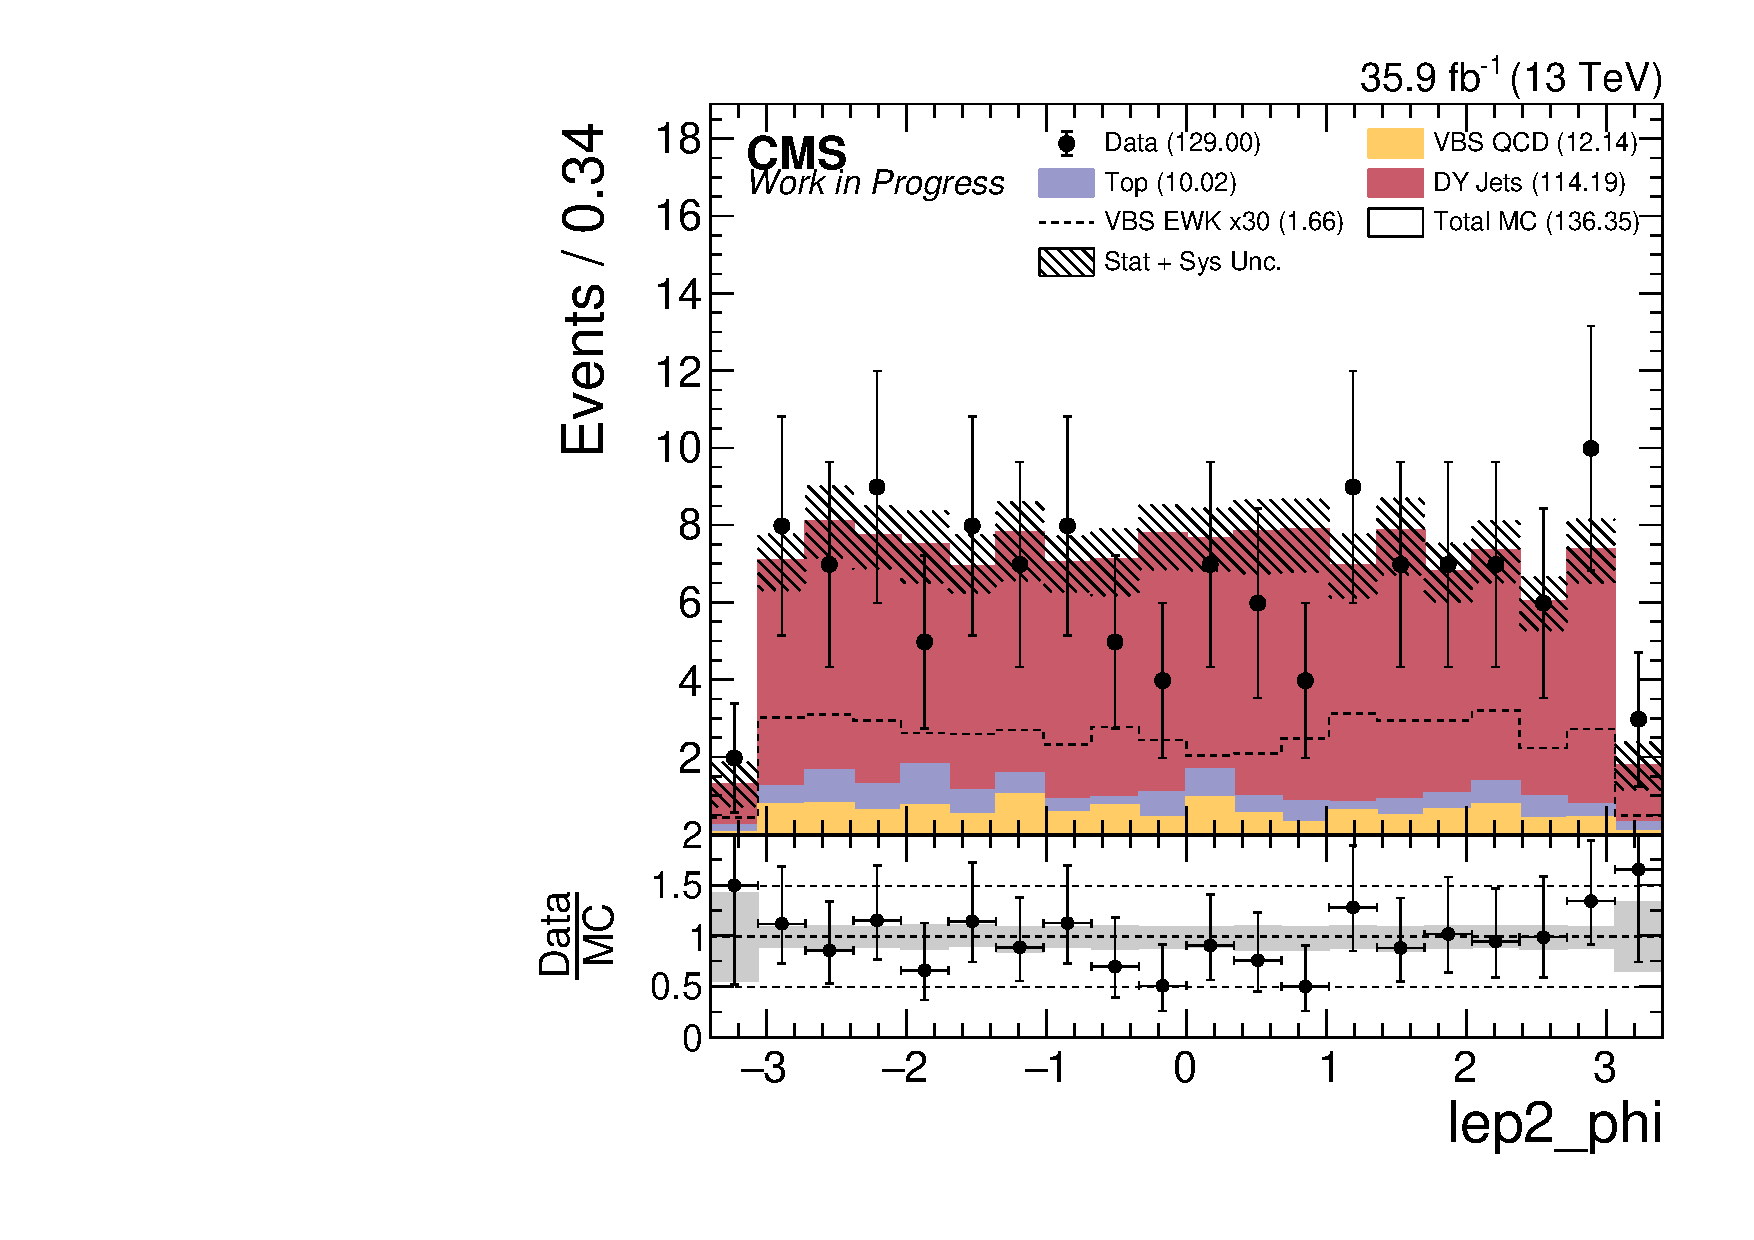
\includegraphics[width=0.30\textwidth]{analysis_plots/2016_zv/cr_vjets_e/lep2_phi.pdf}
  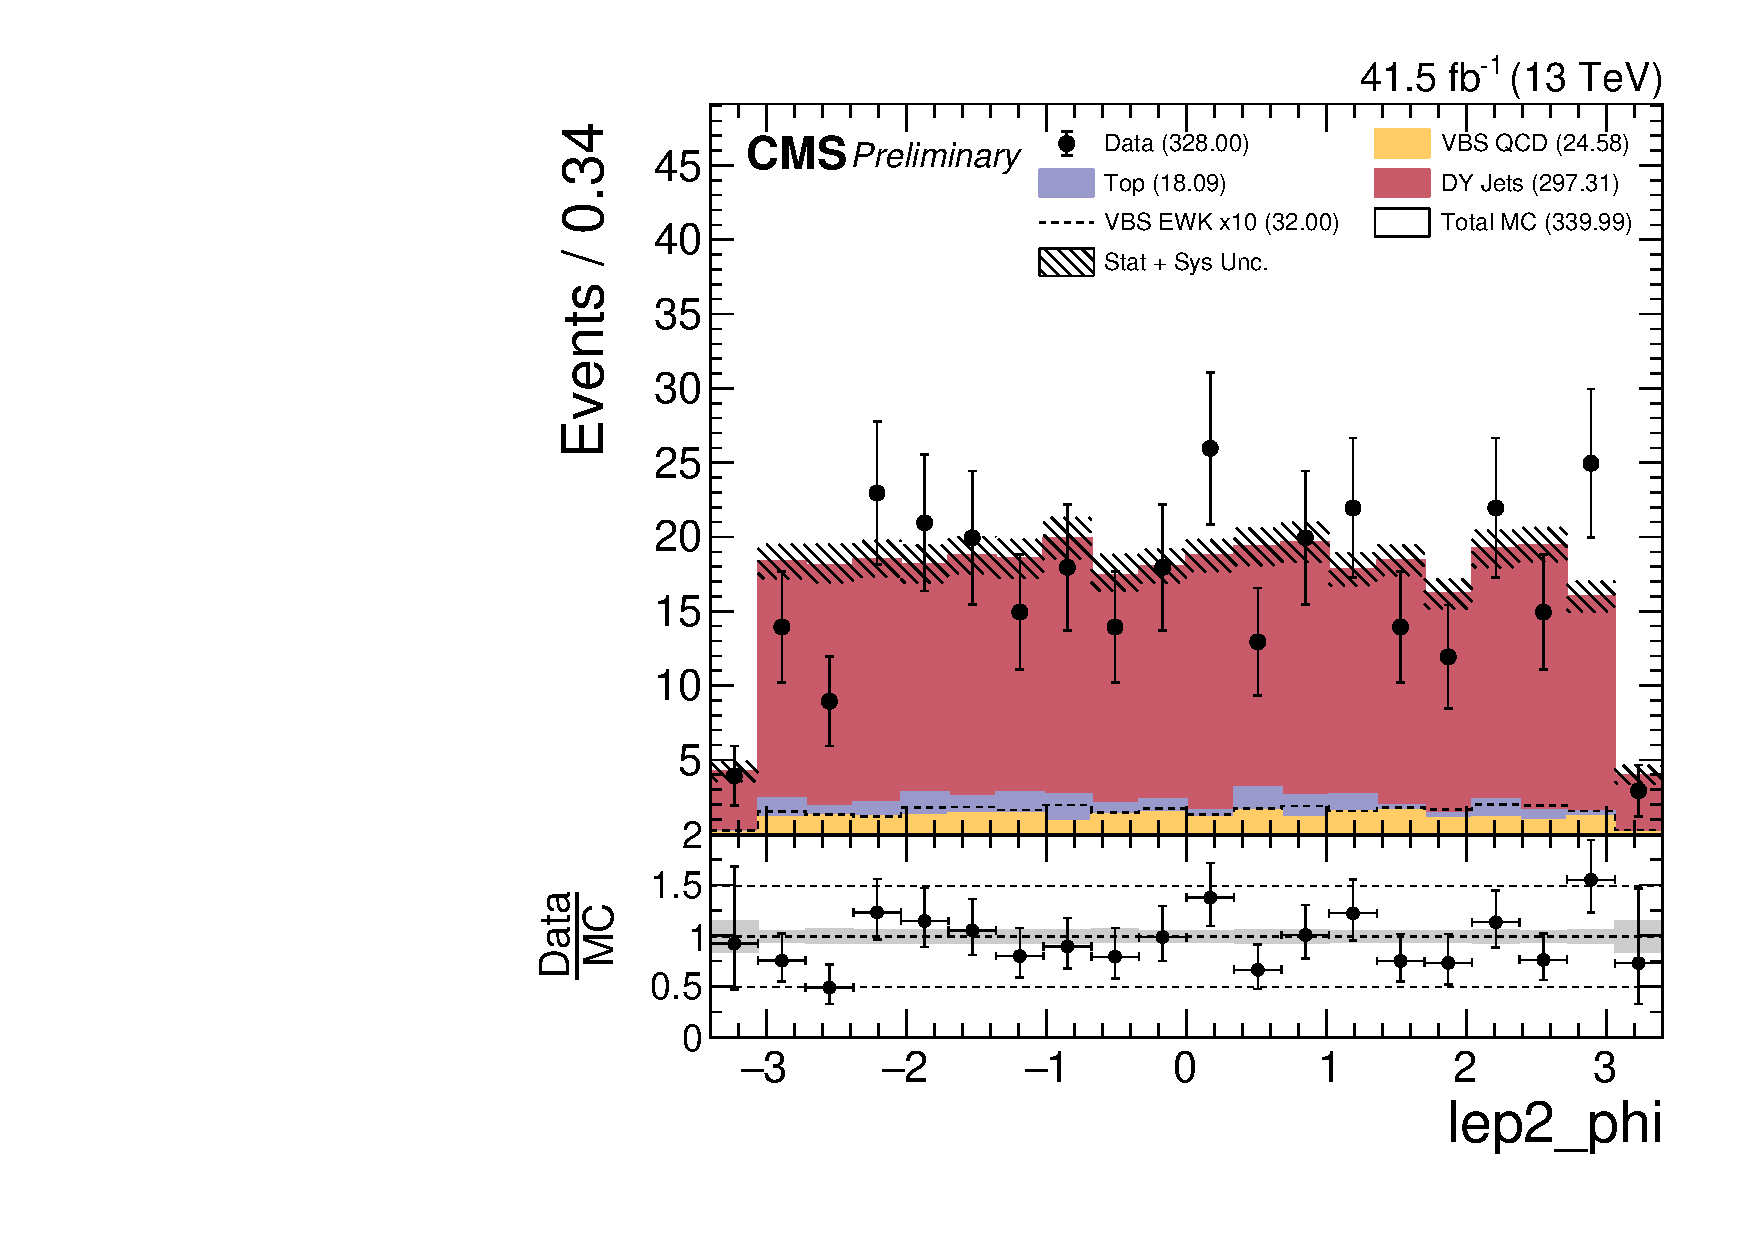
\includegraphics[width=0.30\textwidth]{analysis_plots/2017_zv/cr_vjets_e/lep2_phi.pdf}
  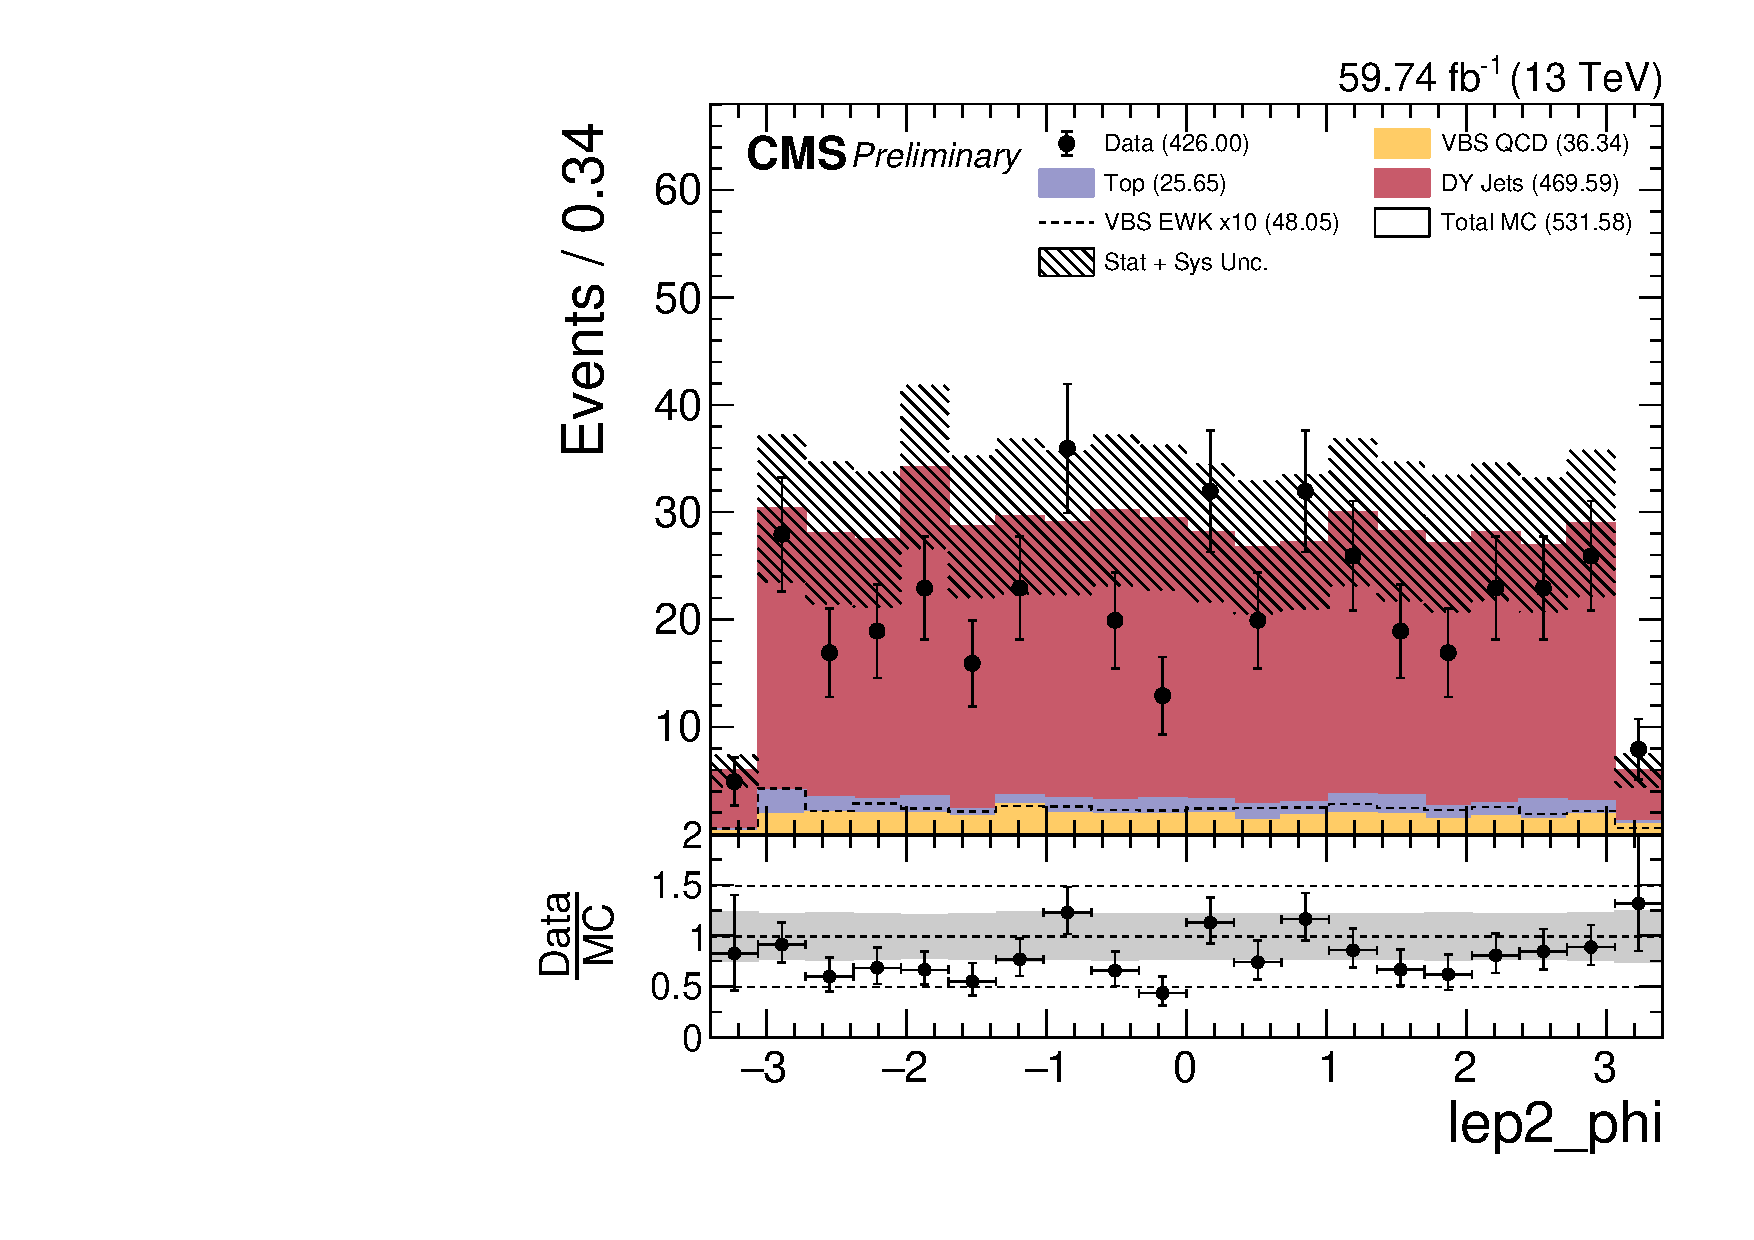
\includegraphics[width=0.30\textwidth]{analysis_plots/2018_zv/cr_vjets_e/lep2_phi.pdf} \\
  \caption[DY+Jets Control Region: Trailing electron kinematics in Boosted ZV Channel]%
  {DY+Jets Control Region: Trailing electron kinematics in Boosted ZV Channel. From Left to Right: 2016,
    2017, and 2018. From Top to Bottom: \( p_T \), \( \eta \), \( \phi \).}%
  \label{fig:zv-cr-vjets-e-lep2-pt-eta-phi}
\end{figure}

\begin{figure}[!ht]
  \centering
  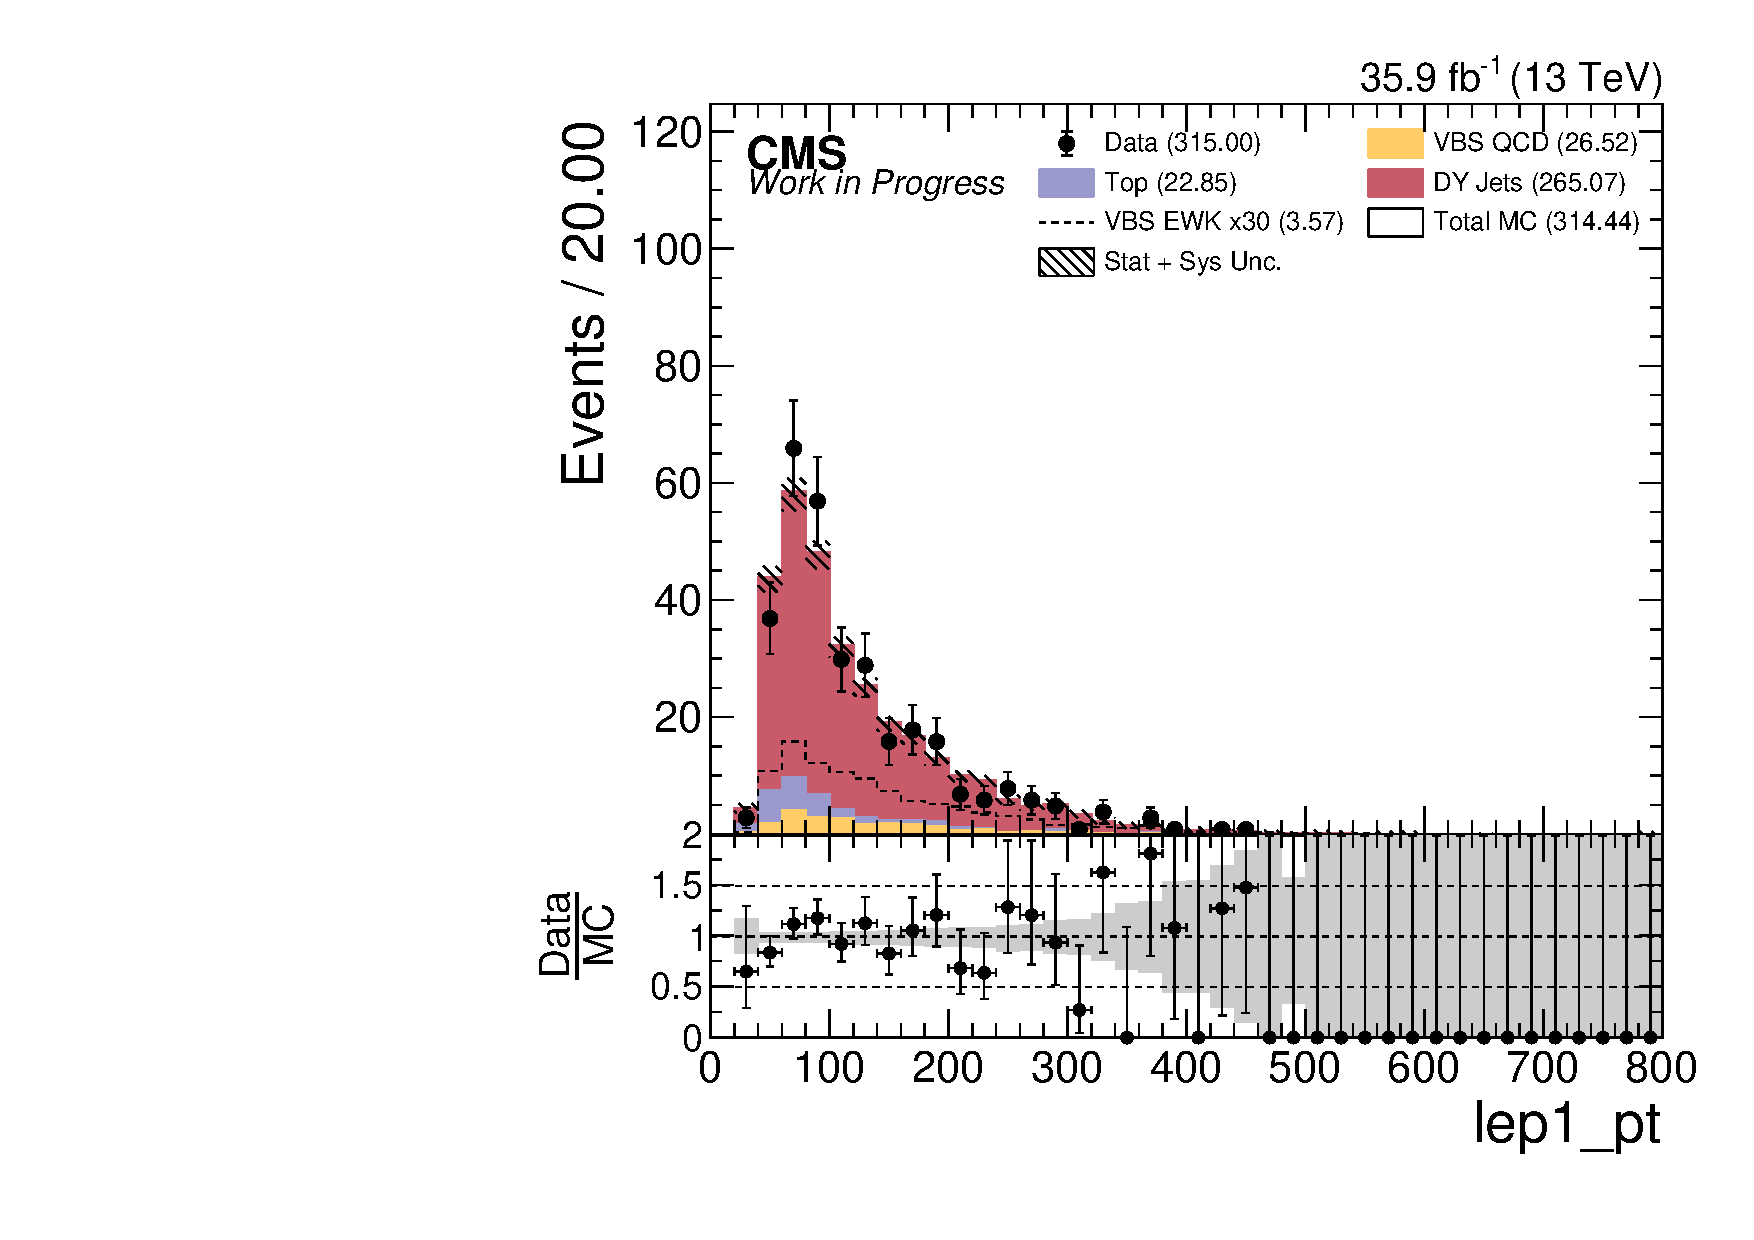
\includegraphics[width=0.30\textwidth]{analysis_plots/2016_zv/cr_vjets_m/lep1_pt.pdf}
  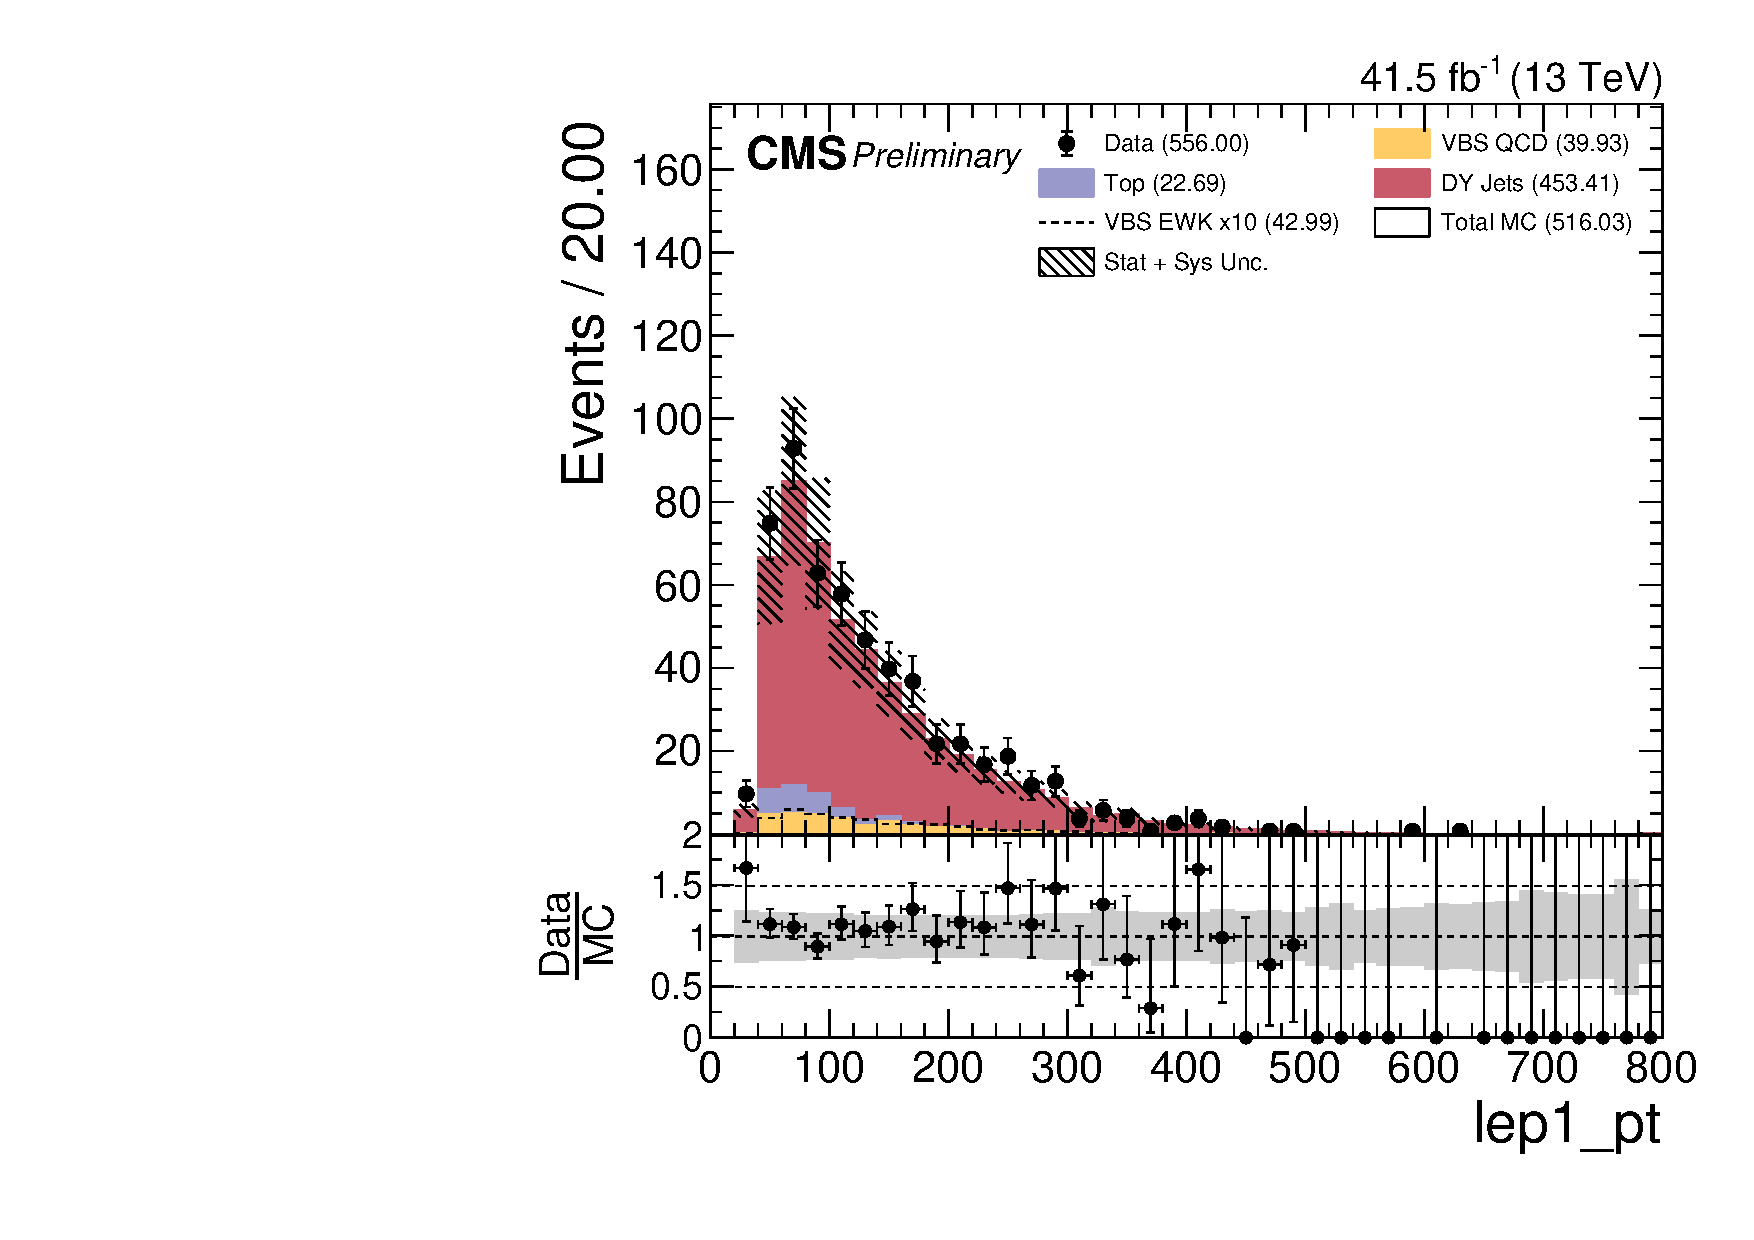
\includegraphics[width=0.30\textwidth]{analysis_plots/2017_zv/cr_vjets_m/lep1_pt.pdf}
  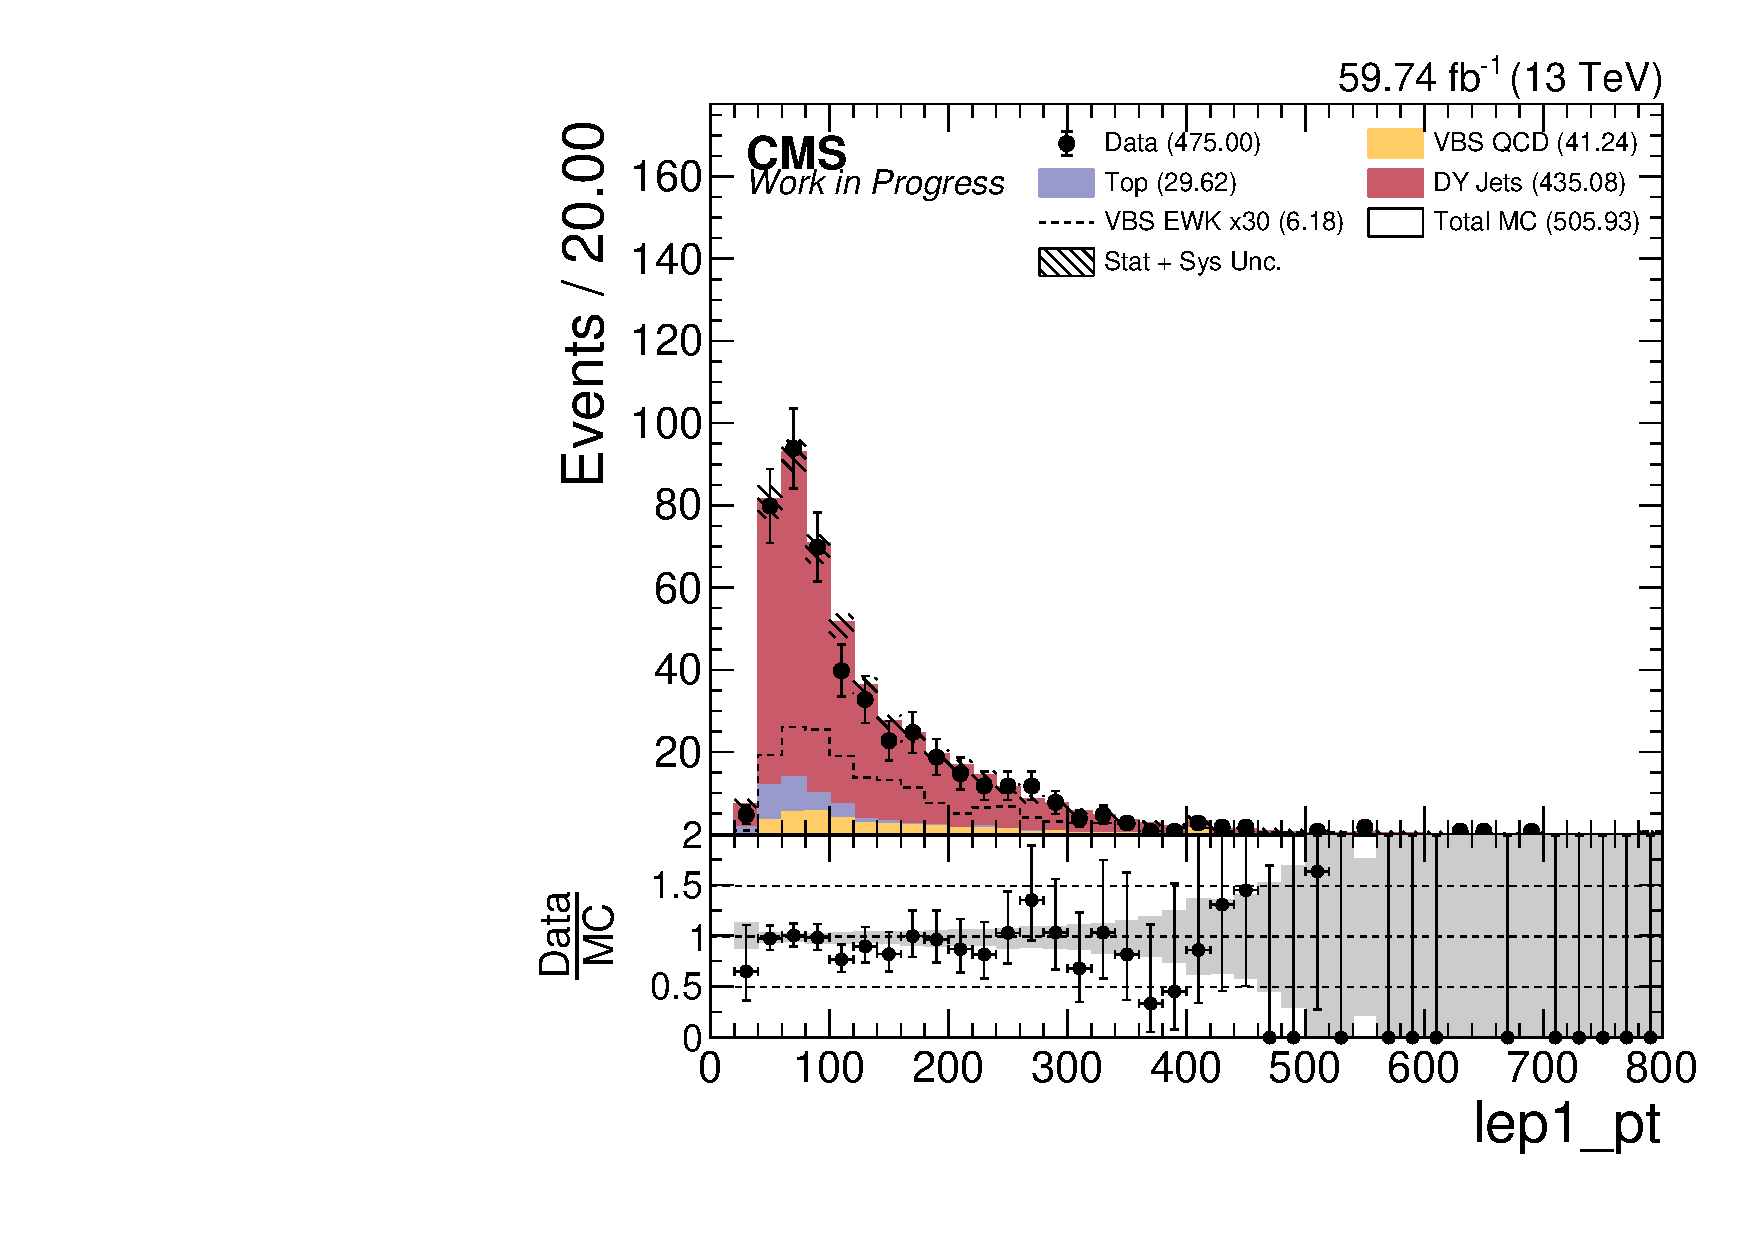
\includegraphics[width=0.30\textwidth]{analysis_plots/2018_zv/cr_vjets_m/lep1_pt.pdf} \\
  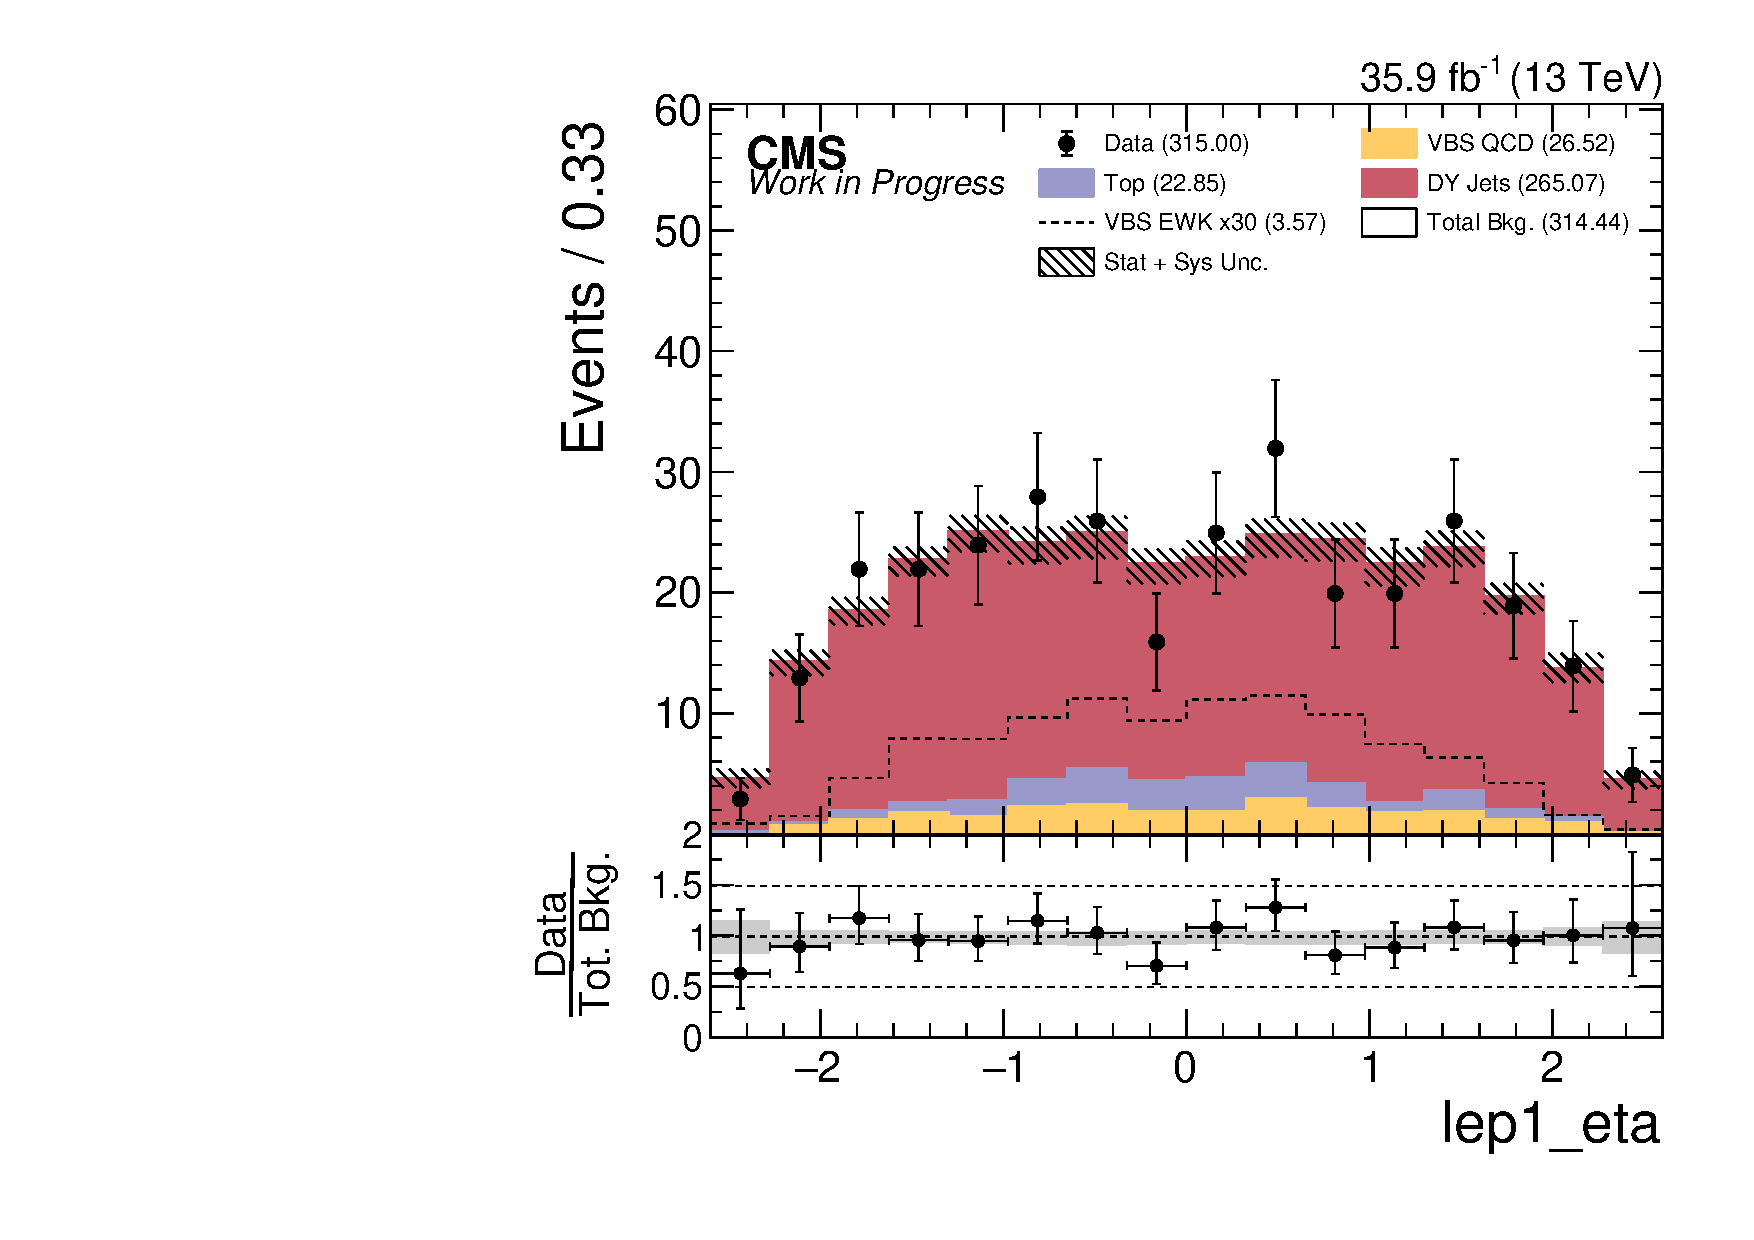
\includegraphics[width=0.30\textwidth]{analysis_plots/2016_zv/cr_vjets_m/lep1_eta.pdf}
  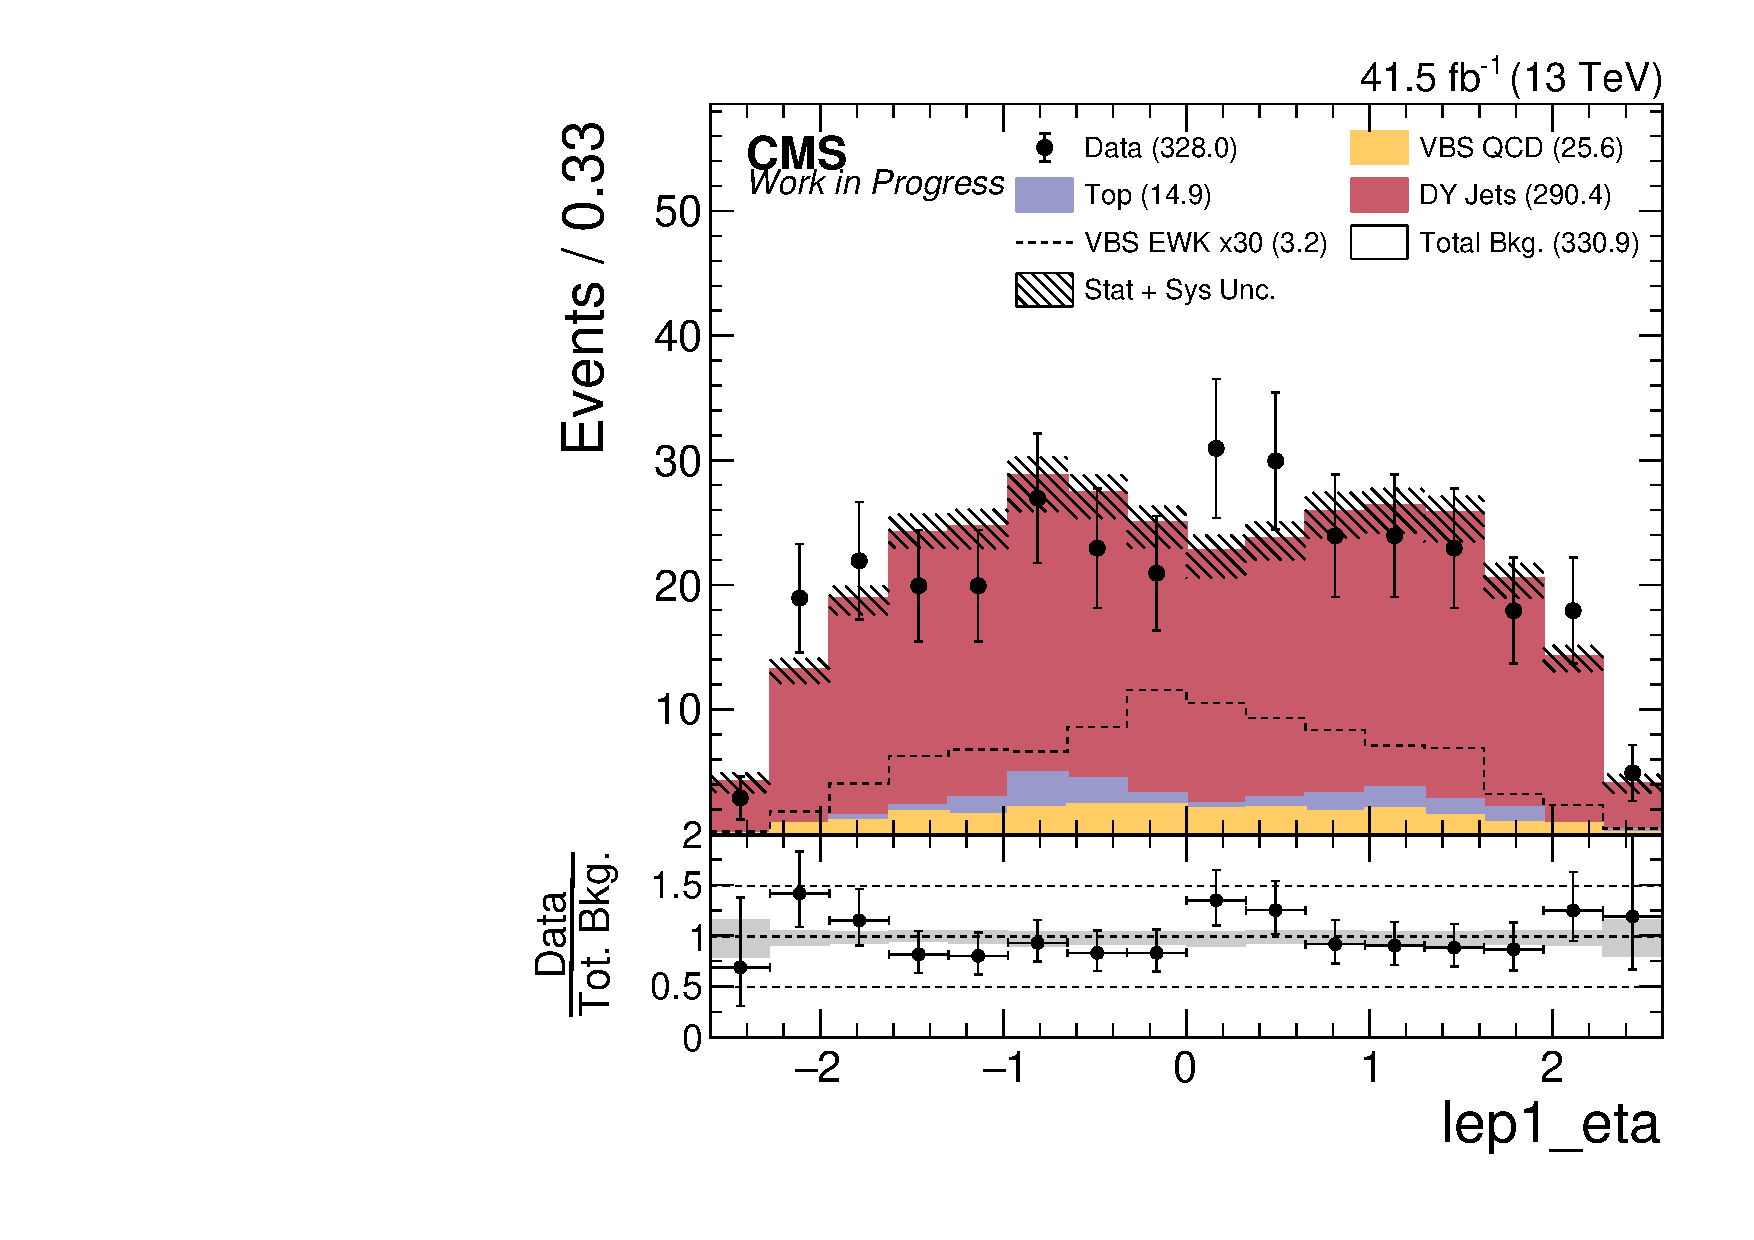
\includegraphics[width=0.30\textwidth]{analysis_plots/2017_zv/cr_vjets_m/lep1_eta.pdf}
  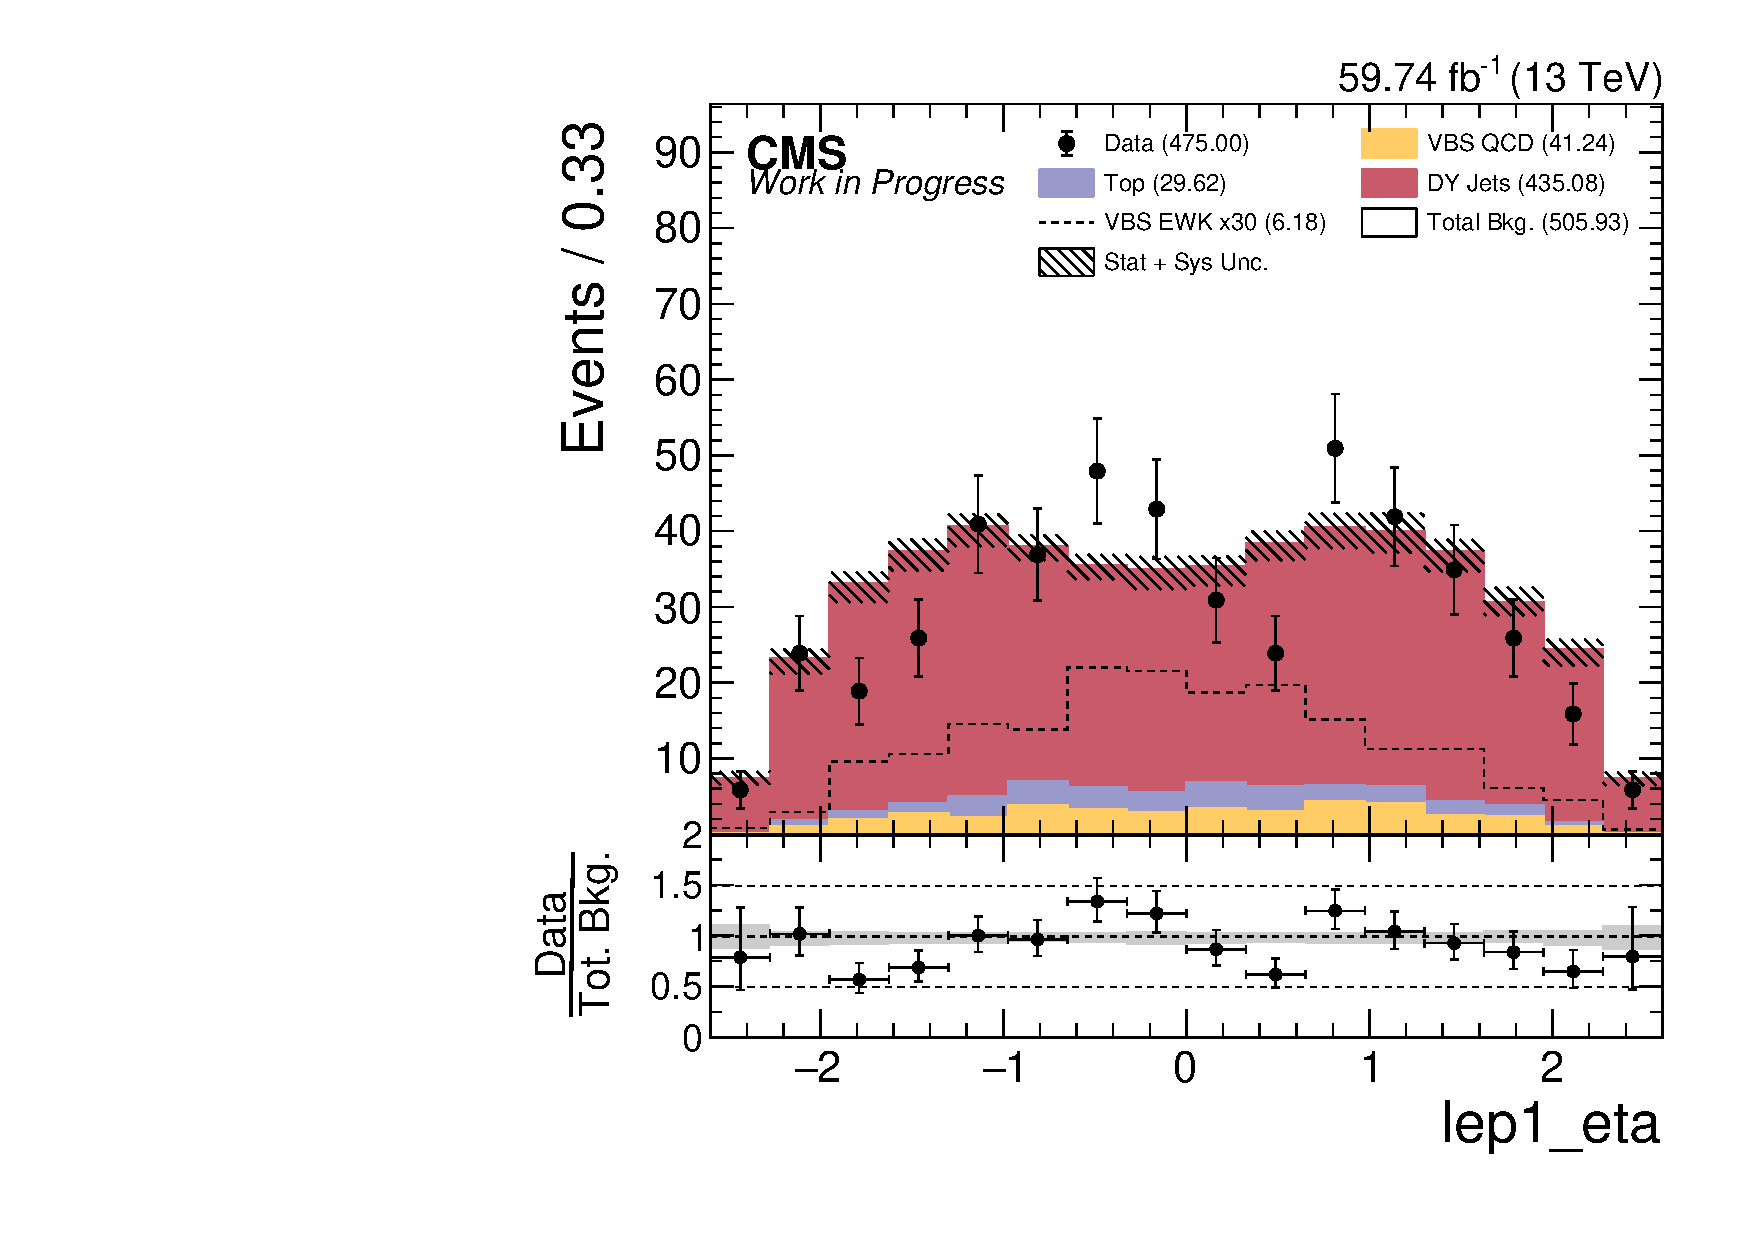
\includegraphics[width=0.30\textwidth]{analysis_plots/2018_zv/cr_vjets_m/lep1_eta.pdf} \\
  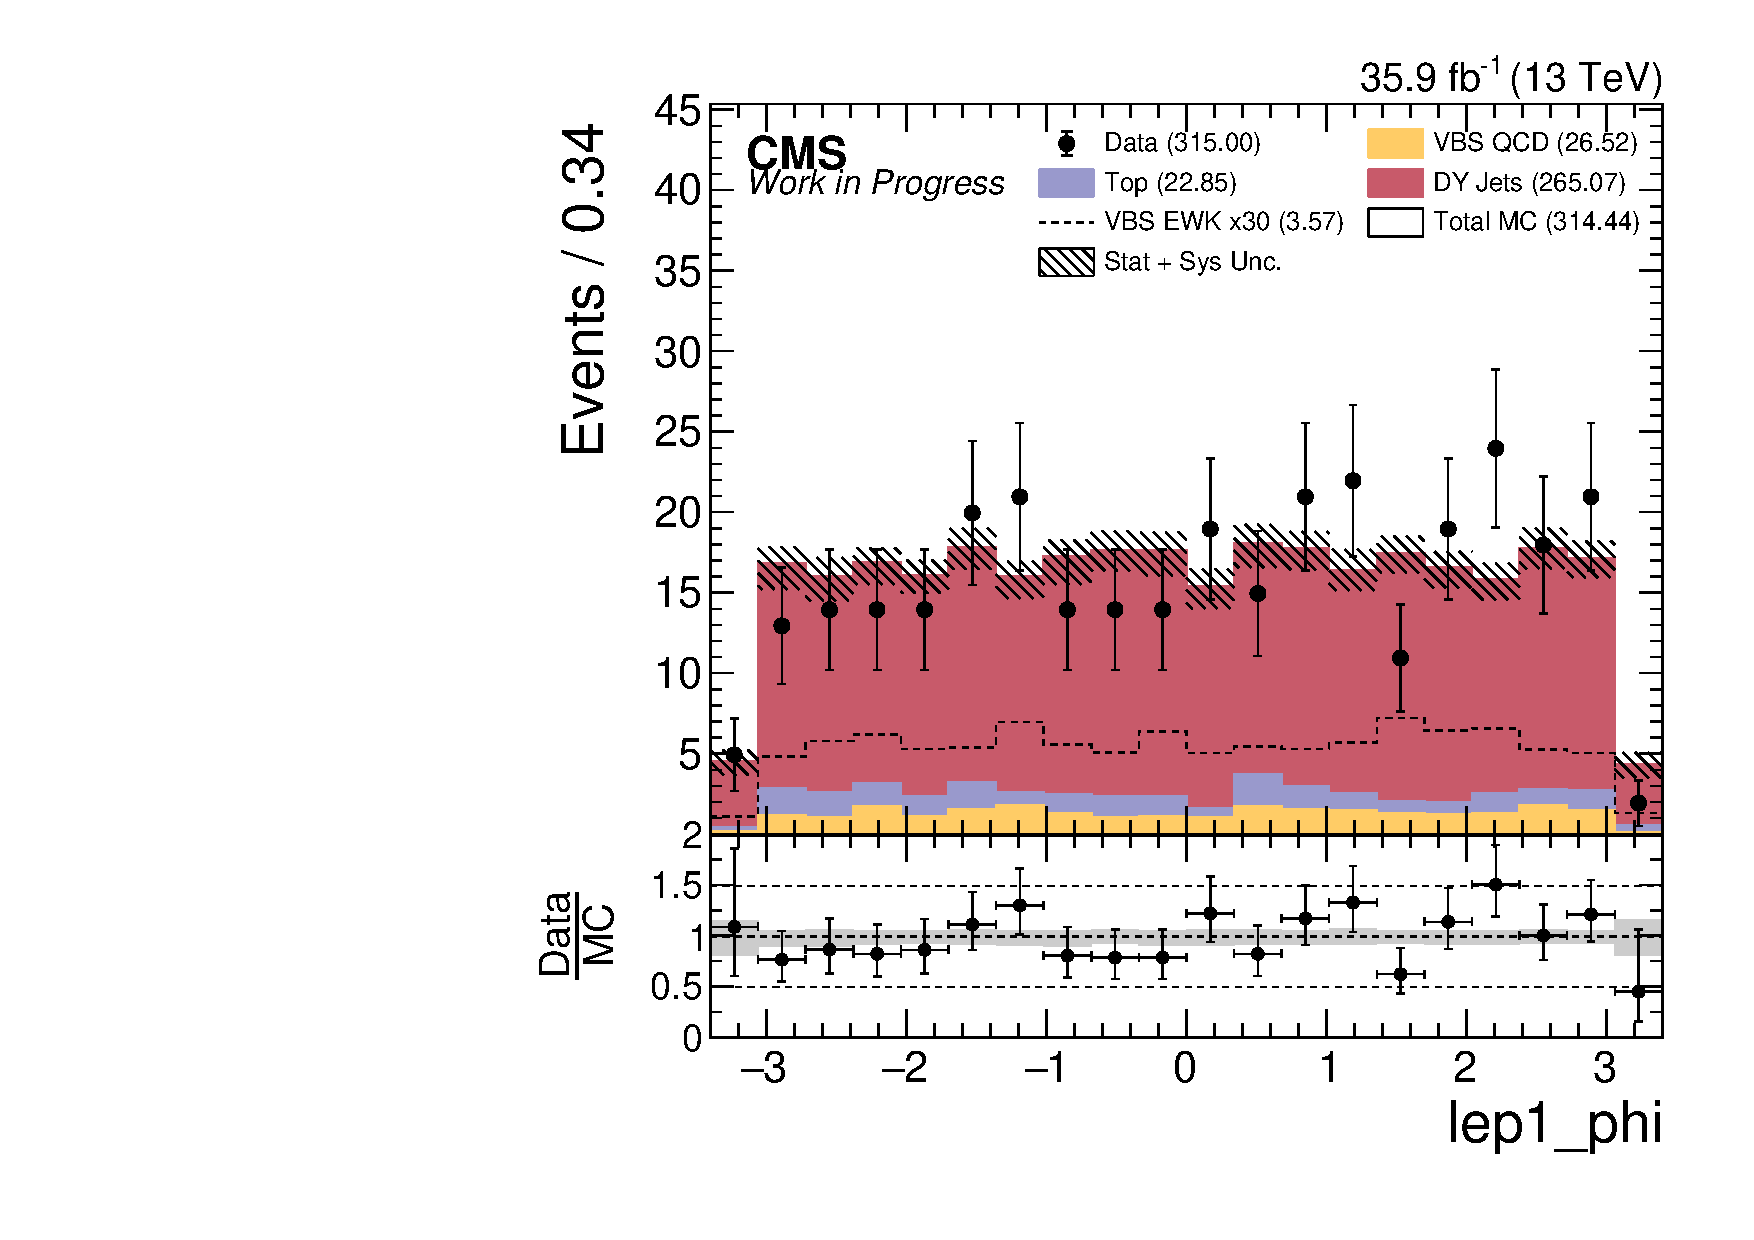
\includegraphics[width=0.30\textwidth]{analysis_plots/2016_zv/cr_vjets_m/lep1_phi.pdf}
  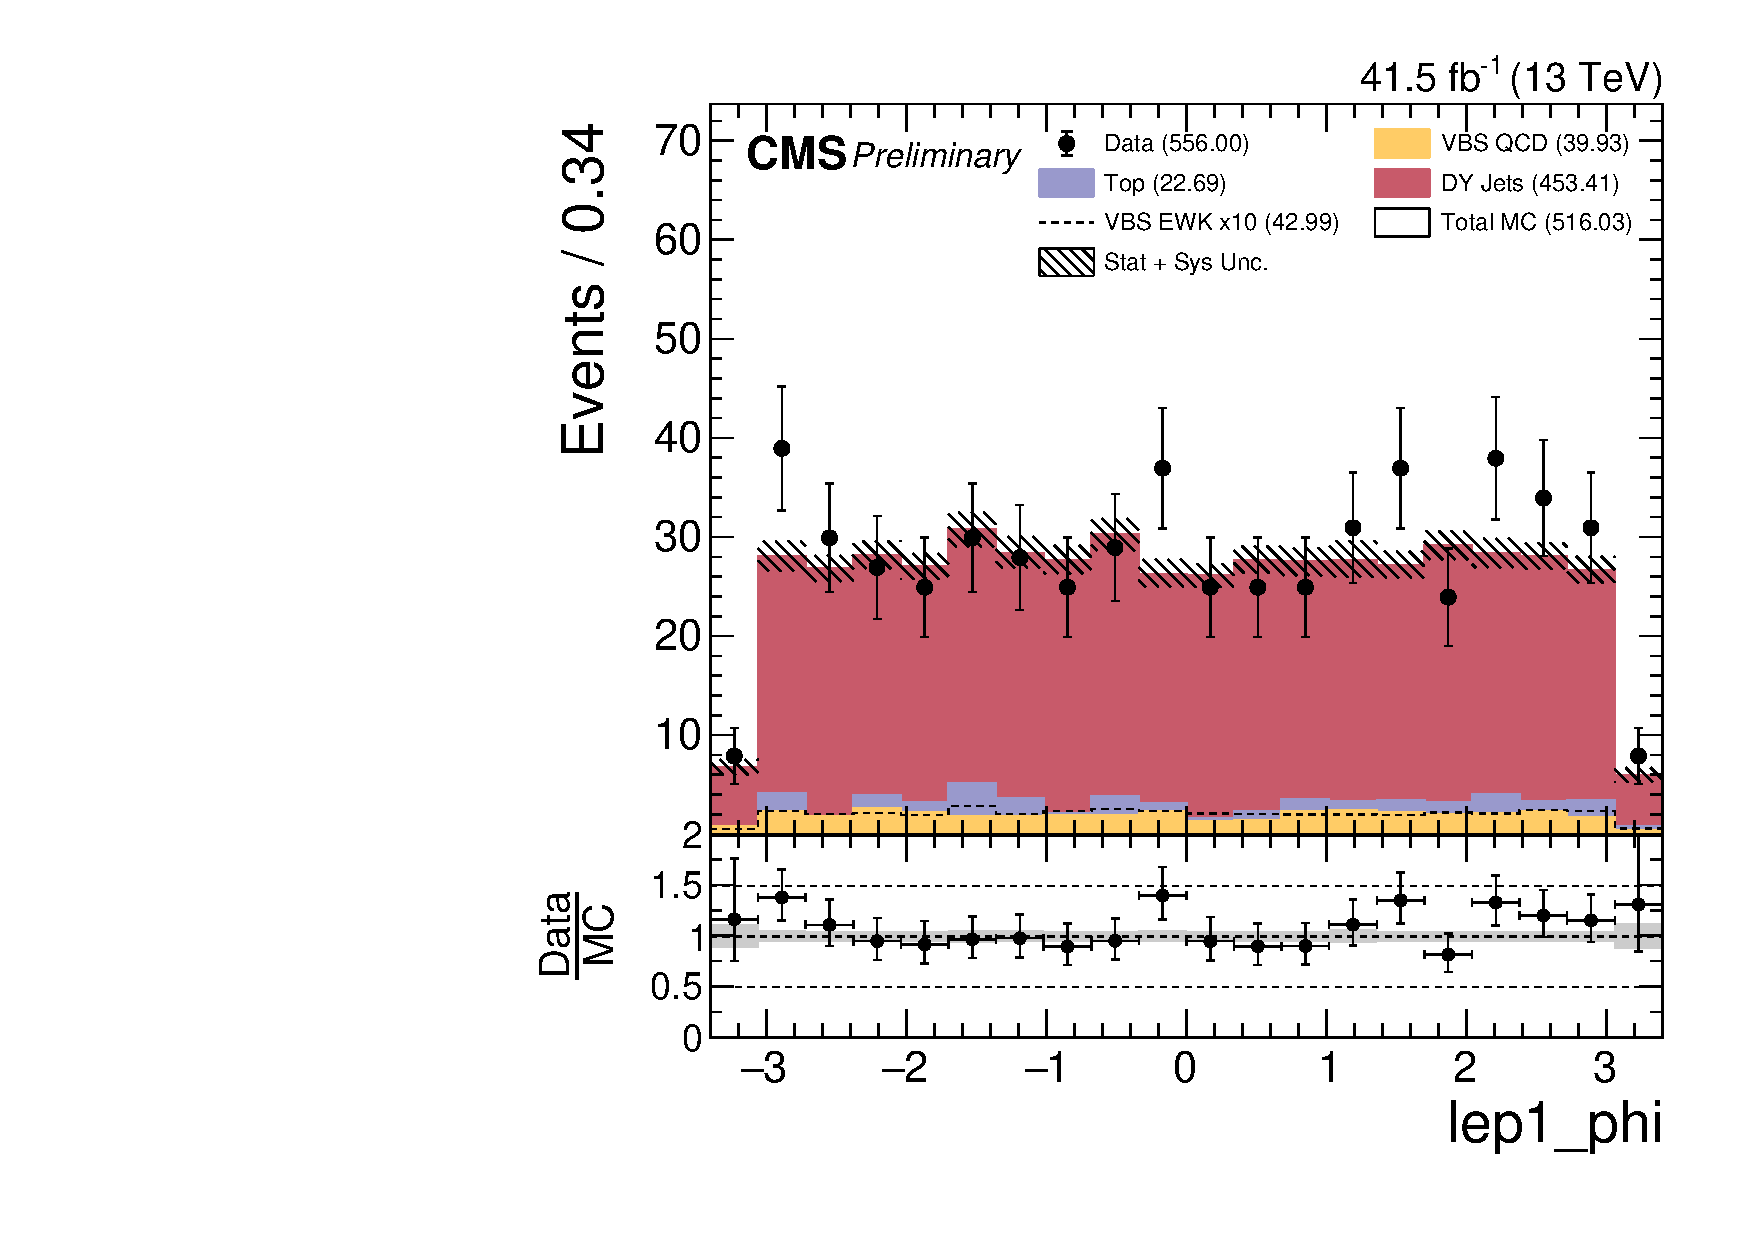
\includegraphics[width=0.30\textwidth]{analysis_plots/2017_zv/cr_vjets_m/lep1_phi.pdf}
  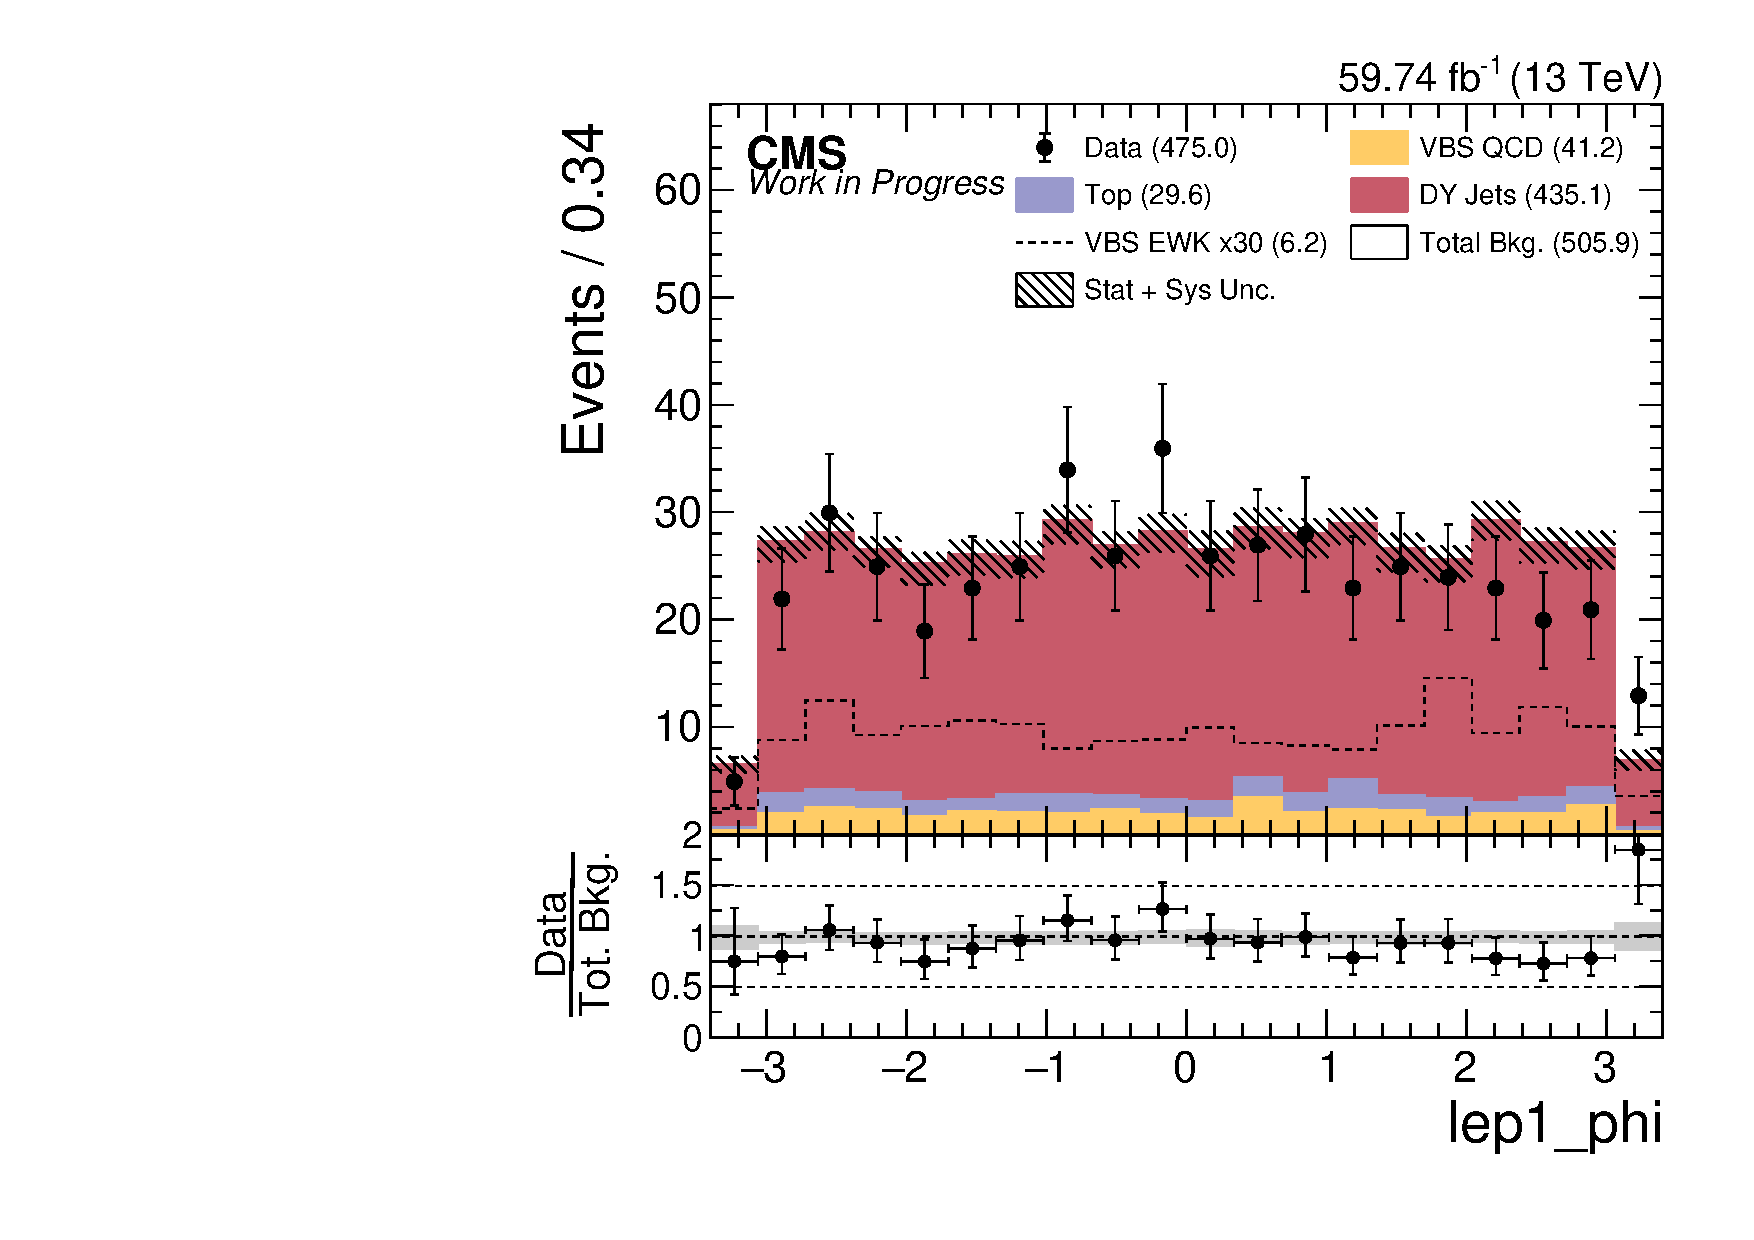
\includegraphics[width=0.30\textwidth]{analysis_plots/2018_zv/cr_vjets_m/lep1_phi.pdf} \\
  \caption[DY+Jets Control Region: Leading muon kinematics in Boosted ZV Channel]%
  {DY+Jets Control Region: Leading muon kinematics in Boosted ZV Channel. From Left to Right: 2016,
    2017, and 2018. From Top to Bottom: \( p_T \), \( \eta \), \( \phi \).}%
  \label{fig:zv-cr-vjets-m-lep1-pt-eta-phi}
\end{figure}

\begin{figure}[!ht]
  \centering
  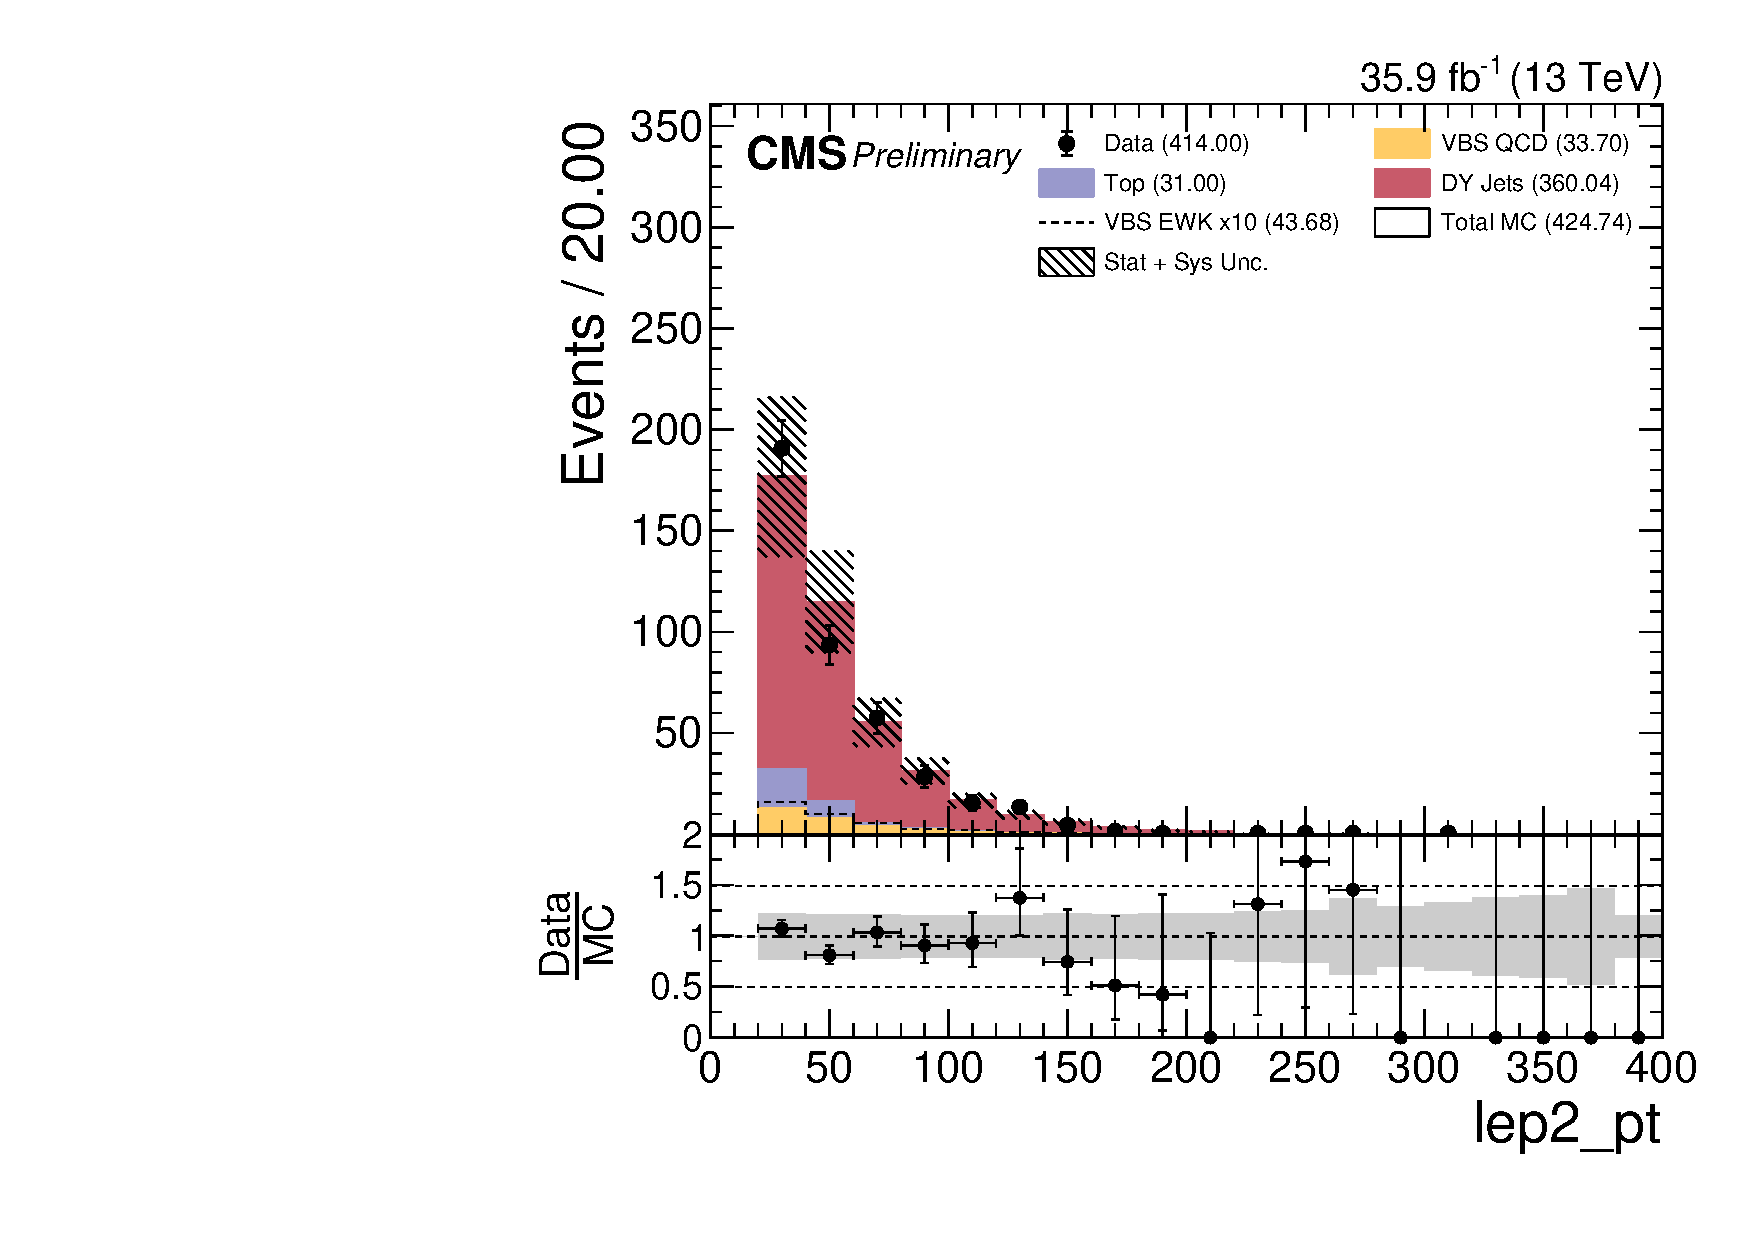
\includegraphics[width=0.30\textwidth]{analysis_plots/2016_zv/cr_vjets_m/lep2_pt.pdf}
  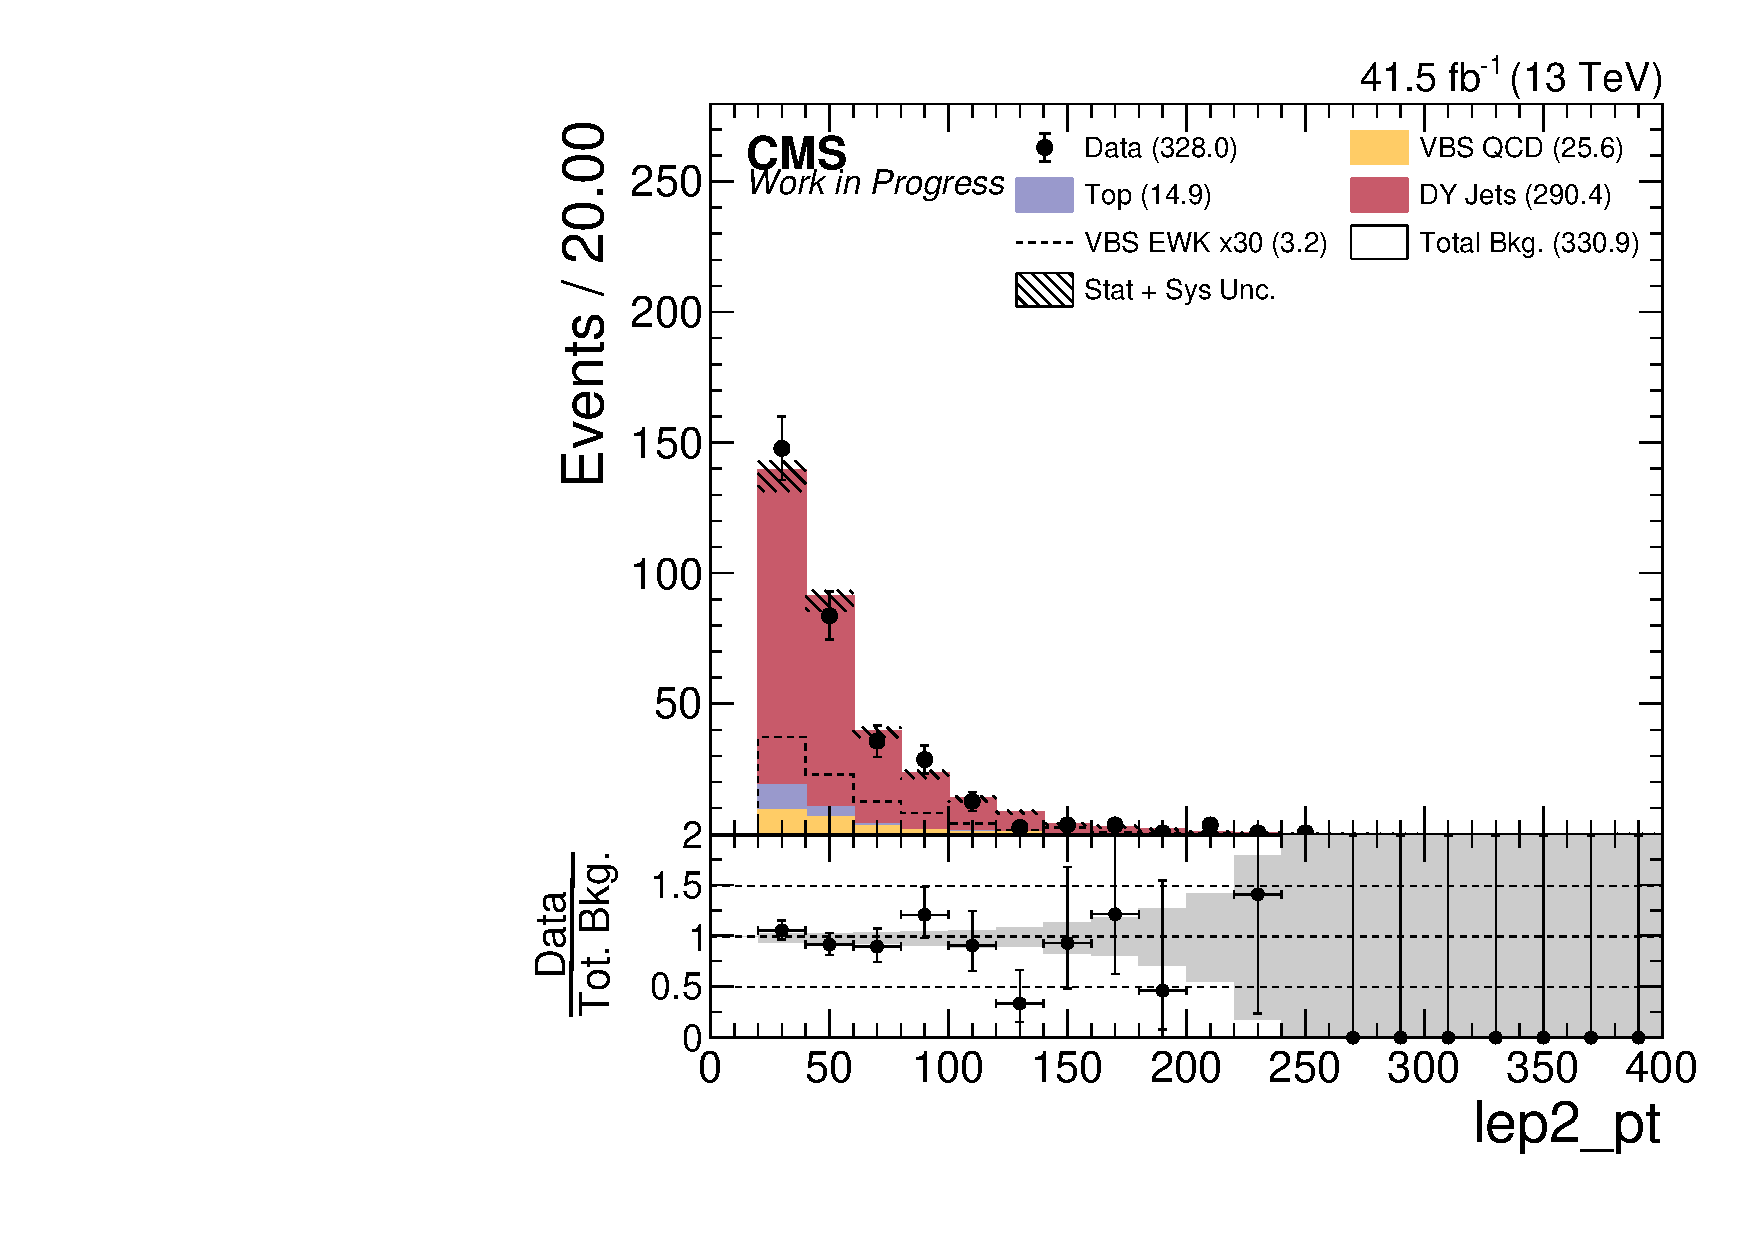
\includegraphics[width=0.30\textwidth]{analysis_plots/2017_zv/cr_vjets_m/lep2_pt.pdf}
  \includegraphics[width=0.30\textwidth]{analysis_plots/2018_zv/cr_vjets_m/lep2_pt.pdf} \\
  \includegraphics[width=0.30\textwidth]{analysis_plots/2016_zv/cr_vjets_m/lep2_eta.pdf}
  \includegraphics[width=0.30\textwidth]{analysis_plots/2017_zv/cr_vjets_m/lep2_eta.pdf}
  \includegraphics[width=0.30\textwidth]{analysis_plots/2018_zv/cr_vjets_m/lep2_eta.pdf} \\
  \includegraphics[width=0.30\textwidth]{analysis_plots/2016_zv/cr_vjets_m/lep2_phi.pdf}
  \includegraphics[width=0.30\textwidth]{analysis_plots/2017_zv/cr_vjets_m/lep2_phi.pdf}
  \includegraphics[width=0.30\textwidth]{analysis_plots/2018_zv/cr_vjets_m/lep2_phi.pdf} \\
  \caption[DY+Jets Control Region: Trailing muon kinematics in Boosted ZV Channel]%
  {DY+Jets Control Region: Trailing muon kinematics in Boosted ZV Channel. From Left to Right: 2016,
    2017, and 2018. From Top to Bottom: \( p_T \), \( \eta \), \( \phi \).}%
  \label{fig:zv-cr-vjets-m-lep2-pt-eta-phi}
\end{figure}

\begin{figure}[!ht]
  \centering
  \includegraphics[width=0.30\textwidth]{analysis_plots/2016_zv/cr_vjets_l/fatjet_pt.pdf}
  \includegraphics[width=0.30\textwidth]{analysis_plots/2017_zv/cr_vjets_l/fatjet_pt.pdf}
  \includegraphics[width=0.30\textwidth]{analysis_plots/2018_zv/cr_vjets_l/fatjet_pt.pdf} \\
  \includegraphics[width=0.30\textwidth]{analysis_plots/2016_zv/cr_vjets_l/fatjet_eta.pdf}
  \includegraphics[width=0.30\textwidth]{analysis_plots/2017_zv/cr_vjets_l/fatjet_eta.pdf}
  \includegraphics[width=0.30\textwidth]{analysis_plots/2018_zv/cr_vjets_l/fatjet_eta.pdf} \\
  \includegraphics[width=0.30\textwidth]{analysis_plots/2016_zv/cr_vjets_l/fatjet_m.pdf}
  \includegraphics[width=0.30\textwidth]{analysis_plots/2017_zv/cr_vjets_l/fatjet_m.pdf}
  \includegraphics[width=0.30\textwidth]{analysis_plots/2018_zv/cr_vjets_l/fatjet_m.pdf} \\
  \caption[DY+Jets Control Region: Hadronic boson kinematics in Boosted ZV Channel]%
  {DY+Jets Control Region: Hadronic boson kinematics in Boosted ZV Channel. From Left to Right: 2016,
    2017, and 2018. From Top to Bottom: \( p_T \), \( \eta \), mass \( m \).}%
  \label{fig:zv-cr-vjets-l-fatjet-pt-eta-m}
\end{figure}

\begin{figure}[!ht]
  \centering
  \includegraphics[width=0.30\textwidth]{analysis_plots/2016_zv/cr_vjets_l/vbf_j1_pt.pdf}
  \includegraphics[width=0.30\textwidth]{analysis_plots/2017_zv/cr_vjets_l/vbf_j1_pt.pdf}
  \includegraphics[width=0.30\textwidth]{analysis_plots/2018_zv/cr_vjets_l/vbf_j1_pt.pdf} \\
  \includegraphics[width=0.30\textwidth]{analysis_plots/2016_zv/cr_vjets_l/vbf_j1_eta.pdf}
  \includegraphics[width=0.30\textwidth]{analysis_plots/2017_zv/cr_vjets_l/vbf_j1_eta.pdf}
  \includegraphics[width=0.30\textwidth]{analysis_plots/2018_zv/cr_vjets_l/vbf_j1_eta.pdf} \\
  \includegraphics[width=0.30\textwidth]{analysis_plots/2016_zv/cr_vjets_l/vbf_j1_phi.pdf}
  \includegraphics[width=0.30\textwidth]{analysis_plots/2017_zv/cr_vjets_l/vbf_j1_phi.pdf}
  \includegraphics[width=0.30\textwidth]{analysis_plots/2018_zv/cr_vjets_l/vbf_j1_phi.pdf} \\
  \caption[DY+Jets Control Region: Leading VBS tagged jet kinematics in Boosted ZV Channel]%
  {DY+Jets Control Region: Leading VBS tagged jet kinematics in Boosted ZV Channel. From Left to Right: 2016,
    2017, and 2018. From Top to Bottom: \( p_T \), \( \eta \), \( \phi \).}%
  \label{fig:zv-cr-vjets-l-vbs1-pt-eta-m}
\end{figure}

\begin{figure}[!ht]
  \centering
  \includegraphics[width=0.30\textwidth]{analysis_plots/2016_zv/cr_vjets_l/vbf_j2_pt.pdf}
  \includegraphics[width=0.30\textwidth]{analysis_plots/2017_zv/cr_vjets_l/vbf_j2_pt.pdf}
  \includegraphics[width=0.30\textwidth]{analysis_plots/2018_zv/cr_vjets_l/vbf_j2_pt.pdf} \\
  \includegraphics[width=0.30\textwidth]{analysis_plots/2016_zv/cr_vjets_l/vbf_j2_eta.pdf}
  \includegraphics[width=0.30\textwidth]{analysis_plots/2017_zv/cr_vjets_l/vbf_j2_eta.pdf}
  \includegraphics[width=0.30\textwidth]{analysis_plots/2018_zv/cr_vjets_l/vbf_j2_eta.pdf} \\
  \includegraphics[width=0.30\textwidth]{analysis_plots/2016_zv/cr_vjets_l/vbf_j2_phi.pdf}
  \includegraphics[width=0.30\textwidth]{analysis_plots/2017_zv/cr_vjets_l/vbf_j2_phi.pdf}
  \includegraphics[width=0.30\textwidth]{analysis_plots/2018_zv/cr_vjets_l/vbf_j2_phi.pdf} \\
  \caption[DY+Jets Control Region: Trailing VBS tagged jet kinematics in Boosted ZV Channel]%
  {DY+Jets Control Region: Trailing VBS tagged jet kinematics in Boosted ZV Channel. From Left to Right: 2016,
    2017, and 2018. From Top to Bottom: \( p_T \), \( \eta \), \( \phi \).}%
  \label{fig:zv-cr-vjets-l-vbs2-pt-eta-m}
\end{figure}

\clearpage
\subsection{
  Resolved ZV DY+Jets Control Region
}

\begin{figure}[!ht]
  \centering
  \includegraphics[width=0.30\textwidth]{analysis_plots/2016_zjj/cr_vjets_e/lep1_pt.pdf}
  \includegraphics[width=0.30\textwidth]{analysis_plots/2017_zjj/cr_vjets_e/lep1_pt.pdf}
  \includegraphics[width=0.30\textwidth]{analysis_plots/2018_zjj/cr_vjets_e/lep1_pt.pdf} \\
  \includegraphics[width=0.30\textwidth]{analysis_plots/2016_zjj/cr_vjets_e/lep1_eta.pdf}
  \includegraphics[width=0.30\textwidth]{analysis_plots/2017_zjj/cr_vjets_e/lep1_eta.pdf}
  \includegraphics[width=0.30\textwidth]{analysis_plots/2018_zjj/cr_vjets_e/lep1_eta.pdf} \\
  \includegraphics[width=0.30\textwidth]{analysis_plots/2016_zjj/cr_vjets_e/lep1_phi.pdf}
  \includegraphics[width=0.30\textwidth]{analysis_plots/2017_zjj/cr_vjets_e/lep1_phi.pdf}
  \includegraphics[width=0.30\textwidth]{analysis_plots/2018_zjj/cr_vjets_e/lep1_phi.pdf} \\
  \caption[DY+Jets Control Region: Leading electron kinematics in Resolved ZV Channel]%
  {DY+Jets Control Region: Leading electron kinematics in Resolved ZV Channel. From Left to Right: 2016,
    2017, and 2018. From Top to Bottom: \( p_T \), \( \eta \), \( \phi \).}%
  \label{fig:zjj-cr-vjets-e-lep1-pt-eta-phi}
\end{figure}

\begin{figure}[!ht]
  \centering
  \includegraphics[width=0.30\textwidth]{analysis_plots/2016_zjj/cr_vjets_e/lep2_pt.pdf}
  \includegraphics[width=0.30\textwidth]{analysis_plots/2017_zjj/cr_vjets_e/lep2_pt.pdf}
  \includegraphics[width=0.30\textwidth]{analysis_plots/2018_zjj/cr_vjets_e/lep2_pt.pdf} \\
  \includegraphics[width=0.30\textwidth]{analysis_plots/2016_zjj/cr_vjets_e/lep2_eta.pdf}
  \includegraphics[width=0.30\textwidth]{analysis_plots/2017_zjj/cr_vjets_e/lep2_eta.pdf}
  \includegraphics[width=0.30\textwidth]{analysis_plots/2018_zjj/cr_vjets_e/lep2_eta.pdf} \\
  \includegraphics[width=0.30\textwidth]{analysis_plots/2016_zjj/cr_vjets_e/lep2_phi.pdf}
  \includegraphics[width=0.30\textwidth]{analysis_plots/2017_zjj/cr_vjets_e/lep2_phi.pdf}
  \includegraphics[width=0.30\textwidth]{analysis_plots/2018_zjj/cr_vjets_e/lep2_phi.pdf} \\
  \caption[DY+Jets Control Region: Trailing electron kinematics in Resolved ZV Channel]%
  {DY+Jets Control Region: Trailing electron kinematics in Resolved ZV Channel. From Left to Right: 2016,
    2017, and 2018. From Top to Bottom: \( p_T \), \( \eta \), \( \phi \).}%
  \label{fig:zjj-cr-vjets-e-lep2-pt-eta-phi}
\end{figure}

\begin{figure}[!ht]
  \centering
  \includegraphics[width=0.30\textwidth]{analysis_plots/2016_zjj/cr_vjets_m/lep1_pt.pdf}
  \includegraphics[width=0.30\textwidth]{analysis_plots/2017_zjj/cr_vjets_m/lep1_pt.pdf}
  \includegraphics[width=0.30\textwidth]{analysis_plots/2018_zjj/cr_vjets_m/lep1_pt.pdf} \\
  \includegraphics[width=0.30\textwidth]{analysis_plots/2016_zjj/cr_vjets_m/lep1_eta.pdf}
  \includegraphics[width=0.30\textwidth]{analysis_plots/2017_zjj/cr_vjets_m/lep1_eta.pdf}
  \includegraphics[width=0.30\textwidth]{analysis_plots/2018_zjj/cr_vjets_m/lep1_eta.pdf} \\
  \includegraphics[width=0.30\textwidth]{analysis_plots/2016_zjj/cr_vjets_m/lep1_phi.pdf}
  \includegraphics[width=0.30\textwidth]{analysis_plots/2017_zjj/cr_vjets_m/lep1_phi.pdf}
  \includegraphics[width=0.30\textwidth]{analysis_plots/2018_zjj/cr_vjets_m/lep1_phi.pdf} \\
  \caption[DY+Jets Control Region: Leading muon kinematics in Resolved ZV Channel]%
  {DY+Jets Control Region: Leading muon kinematics in Resolved ZV Channel. From Left to Right: 2016,
    2017, and 2018. From Top to Bottom: \( p_T \), \( \eta \), \( \phi \).}%
  \label{fig:zjj-cr-vjets-m-lep1-pt-eta-phi}
\end{figure}

\begin{figure}[!ht]
  \centering
  \includegraphics[width=0.30\textwidth]{analysis_plots/2016_zjj/cr_vjets_m/lep2_pt.pdf}
  \includegraphics[width=0.30\textwidth]{analysis_plots/2017_zjj/cr_vjets_m/lep2_pt.pdf}
  \includegraphics[width=0.30\textwidth]{analysis_plots/2018_zjj/cr_vjets_m/lep2_pt.pdf} \\
  \includegraphics[width=0.30\textwidth]{analysis_plots/2016_zjj/cr_vjets_m/lep2_eta.pdf}
  \includegraphics[width=0.30\textwidth]{analysis_plots/2017_zjj/cr_vjets_m/lep2_eta.pdf}
  \includegraphics[width=0.30\textwidth]{analysis_plots/2018_zjj/cr_vjets_m/lep2_eta.pdf} \\
  \includegraphics[width=0.30\textwidth]{analysis_plots/2016_zjj/cr_vjets_m/lep2_phi.pdf}
  \includegraphics[width=0.30\textwidth]{analysis_plots/2017_zjj/cr_vjets_m/lep2_phi.pdf}
  \includegraphics[width=0.30\textwidth]{analysis_plots/2018_zjj/cr_vjets_m/lep2_phi.pdf} \\
  \caption[DY+Jets Control Region: Trailing muon kinematics in Resolved ZV Channel]%
  {DY+Jets Control Region: Trailing muon kinematics in Resolved ZV Channel. From Left to Right: 2016,
    2017, and 2018. From Top to Bottom: \( p_T \), \( \eta \), \( \phi \).}%
  \label{fig:zjj-cr-vjets-m-lep2-pt-eta-phi}
\end{figure}

\begin{figure}[!ht]
  \centering
  \includegraphics[width=0.30\textwidth]{analysis_plots/2016_zjj/cr_vjets_l/dijet_j1_pt.pdf}
  \includegraphics[width=0.30\textwidth]{analysis_plots/2017_zjj/cr_vjets_l/dijet_j1_pt.pdf}
  \includegraphics[width=0.30\textwidth]{analysis_plots/2018_zjj/cr_vjets_l/dijet_j1_pt.pdf} \\
  \includegraphics[width=0.30\textwidth]{analysis_plots/2016_zjj/cr_vjets_l/dijet_j1_eta.pdf}
  \includegraphics[width=0.30\textwidth]{analysis_plots/2017_zjj/cr_vjets_l/dijet_j1_eta.pdf}
  \includegraphics[width=0.30\textwidth]{analysis_plots/2018_zjj/cr_vjets_l/dijet_j1_eta.pdf} \\
  \includegraphics[width=0.30\textwidth]{analysis_plots/2016_zjj/cr_vjets_l/dijet_m.pdf}
  \includegraphics[width=0.30\textwidth]{analysis_plots/2017_zjj/cr_vjets_l/dijet_m.pdf}
  \includegraphics[width=0.30\textwidth]{analysis_plots/2018_zjj/cr_vjets_l/dijet_m.pdf} \\
  \caption[DY+Jets Control Region: Hadronic boson leading jet kinematics in Resolved ZV Channel]%
  {DY+Jets Control Region: Hadronic boson leading jet kinematics in Resolved ZV Channel. From Left to Right: 2016,
    2017, and 2018. From Top to Bottom: \( p_T \), \( \eta \), invariant mass \( m_{jj} \).}%
  \label{fig:zjj-cr-vjets-l-dijet1-pt-eta-m}
\end{figure}

\begin{figure}[!ht]
  \centering
  \includegraphics[width=0.30\textwidth]{analysis_plots/2016_zjj/cr_vjets_l/dijet_j2_pt.pdf}
  \includegraphics[width=0.30\textwidth]{analysis_plots/2017_zjj/cr_vjets_l/dijet_j2_pt.pdf}
  \includegraphics[width=0.30\textwidth]{analysis_plots/2018_zjj/cr_vjets_l/dijet_j2_pt.pdf} \\
  \includegraphics[width=0.30\textwidth]{analysis_plots/2016_zjj/cr_vjets_l/dijet_j2_eta.pdf}
  \includegraphics[width=0.30\textwidth]{analysis_plots/2017_zjj/cr_vjets_l/dijet_j2_eta.pdf}
  \includegraphics[width=0.30\textwidth]{analysis_plots/2018_zjj/cr_vjets_l/dijet_j2_eta.pdf} \\
  \includegraphics[width=0.30\textwidth]{analysis_plots/2016_zjj/cr_vjets_l/dijet_m.pdf}
  \includegraphics[width=0.30\textwidth]{analysis_plots/2017_zjj/cr_vjets_l/dijet_m.pdf}
  \includegraphics[width=0.30\textwidth]{analysis_plots/2018_zjj/cr_vjets_l/dijet_m.pdf} \\
  \caption[DY+Jets Control Region: Hadronic boson trailing jet kinematics in Resolved ZV Channel]%
  {DY+Jets Control Region: Hadronic boson trailing jet kinematics in Resolved ZV Channel. From Left to Right: 2016,
    2017, and 2018. From Top to Bottom: \( p_T \), \( \eta \), invariant mass \( m_{jj} \).}%
  \label{fig:zjj-cr-vjets-l-dijet2-pt-eta-m}
\end{figure}

\begin{figure}[!ht]
  \centering
  \includegraphics[width=0.30\textwidth]{analysis_plots/2016_zjj/cr_vjets_l/vbf_j1_pt.pdf}
  \includegraphics[width=0.30\textwidth]{analysis_plots/2017_zjj/cr_vjets_l/vbf_j1_pt.pdf}
  \includegraphics[width=0.30\textwidth]{analysis_plots/2018_zjj/cr_vjets_l/vbf_j1_pt.pdf} \\
  \includegraphics[width=0.30\textwidth]{analysis_plots/2016_zjj/cr_vjets_l/vbf_j1_eta.pdf}
  \includegraphics[width=0.30\textwidth]{analysis_plots/2017_zjj/cr_vjets_l/vbf_j1_eta.pdf}
  \includegraphics[width=0.30\textwidth]{analysis_plots/2018_zjj/cr_vjets_l/vbf_j1_eta.pdf} \\
  \includegraphics[width=0.30\textwidth]{analysis_plots/2016_zjj/cr_vjets_l/vbf_j1_phi.pdf}
  \includegraphics[width=0.30\textwidth]{analysis_plots/2017_zjj/cr_vjets_l/vbf_j1_phi.pdf}
  \includegraphics[width=0.30\textwidth]{analysis_plots/2018_zjj/cr_vjets_l/vbf_j1_phi.pdf} \\
  \caption[DY+Jets Control Region: Leading VBS tagged jet kinematics in Resolved ZV Channel]%
  {DY+Jets Control Region: Leading VBS tagged jet kinematics in Resolved ZV Channel. From Left to Right: 2016,
    2017, and 2018. From Top to Bottom: \( p_T \), \( \eta \), \( \phi \).}%
  \label{fig:zjj-cr-vjets-l-vbs1-pt-eta-m}
\end{figure}

\begin{figure}[!ht]
  \centering
  \includegraphics[width=0.30\textwidth]{analysis_plots/2016_zjj/cr_vjets_l/vbf_j2_pt.pdf}
  \includegraphics[width=0.30\textwidth]{analysis_plots/2017_zjj/cr_vjets_l/vbf_j2_pt.pdf}
  \includegraphics[width=0.30\textwidth]{analysis_plots/2018_zjj/cr_vjets_l/vbf_j2_pt.pdf} \\
  \includegraphics[width=0.30\textwidth]{analysis_plots/2016_zjj/cr_vjets_l/vbf_j2_eta.pdf}
  \includegraphics[width=0.30\textwidth]{analysis_plots/2017_zjj/cr_vjets_l/vbf_j2_eta.pdf}
  \includegraphics[width=0.30\textwidth]{analysis_plots/2018_zjj/cr_vjets_l/vbf_j2_eta.pdf} \\
  \includegraphics[width=0.30\textwidth]{analysis_plots/2016_zjj/cr_vjets_l/vbf_j2_phi.pdf}
  \includegraphics[width=0.30\textwidth]{analysis_plots/2017_zjj/cr_vjets_l/vbf_j2_phi.pdf}
  \includegraphics[width=0.30\textwidth]{analysis_plots/2018_zjj/cr_vjets_l/vbf_j2_phi.pdf} \\
  \caption[DY+Jets Control Region: Trailing VBS tagged jet kinematics in Resolved ZV Channel]%
  {DY+Jets Control Region: Trailing VBS tagged jet kinematics in Resolved ZV Channel. From Left to Right: 2016,
    2017, and 2018. From Top to Bottom: \( p_T \), \( \eta \), \( \phi \).}%
  \label{fig:zjj-cr-vjets-l-vbs2-pt-eta-m}
\end{figure}

\clearpage
\section{
  Machine Learning Modeling
 }

Instead of traditional cut-based analysis, we decided to use \gls{MVA} a.k.a. \gls{ML}
technique to build a signal vs background classifier. The main reasoning behind using
a \gls{MVA} technique is so that we can build a model which can learn our
analysis topology from looser selection regions and still let us keep higher statistics
for final measurement.

\subsection{
  Algorithm: Gradient Boosted Decision Tree
}

Tools used \gls{TMVA} part of \ROOT{} package (FIXME reference). FIXME some details mathematical
details about BDT and specifically gradient BDT\@.

\subsection{
  Training and Results
}

Two models were trained for boosted and resolved topology and
the training was done using combined MC from all years 2016, 2017, 2018
to benefit from larger statistics see Table~\ref{tab:training-stats},
signal MC ``VBS\_EWK'' was trained against background ``DY + Jets LO'' since
that is dominant background in our analysis.
Each models \gls{BDT} hyper-parameters were tunned to prevent under and over-fitting,
and input variables used were also pruned in order of importance and keeping
model metrics \gls{AUC} of \gls{ROC} relatively unaffected. Distribution of final input variables
used in training are shown in Figure~\ref{fig:vbs-training-input-zv} and Figure~\ref{fig:vbs-training-input-zjj}.

\begin{table}[!ht]
  \centering
  \caption{Training and Testing Statistics}
  \begin{tabular}{lllll}%
    \toprule
             &            & \multicolumn{3}{c}{Number of Events}                    \\
    \cmidrule(lr){3-5}
    Channel  & Dataset    & Training                             & Testing & Total  \\
    \midrule
    Boosted  & Signal     & 7404                                 & 7405    & 14809  \\
    Boosted  & Background & 46991                                & 46991   & 93982  \\
    \midrule
    Resolved & Signal     & 23425                                & 23425   & 46850  \\
    Resolved & Background & 209368                               & 209368  & 418736 \\
    \bottomrule
  \end{tabular}\label{tab:training-stats}
\end{table}

\begin{figure}[!ht]
  \centering
  \includegraphics[width=0.4\textwidth]{analysis_plots/tmva_plots/zv_BDTG14_dibos_m.pdf}
  \includegraphics[width=0.4\textwidth]{analysis_plots/tmva_plots/zv_BDTG14_vbf_m.pdf} \\
  \includegraphics[width=0.4\textwidth]{analysis_plots/tmva_plots/zv_BDTG14_vbf1_AK4_qgid.pdf}
  \includegraphics[width=0.4\textwidth]{analysis_plots/tmva_plots/zv_BDTG14_vbf2_AK4_qgid.pdf} \\
  \includegraphics[width=0.4\textwidth]{analysis_plots/tmva_plots/zv_BDTG14_zeppLep_deta.pdf}
  \caption[Inputs Variables for training Boosted ZV BDT Classifier]%
  {Inputs Variables (combined for Run2 MC) for training Boosted ZV BDT Classifier.
    From top: Diboson invariant mass, VBS tagged jets invariant mass, \gls{QGL} of leading
    VBS tagged jet, \gls{QGL} of trailing VBS tagged jet, Zeppenfeld variable of leptonic boson.}%
  \label{fig:vbs-training-input-zv}
\end{figure}

\begin{figure}[!ht]
  \centering
  \includegraphics[width=0.32\textwidth]{analysis_plots/tmva_plots/zjj_BDTG14_dibos_m.pdf}
  \includegraphics[width=0.32\textwidth]{analysis_plots/tmva_plots/zjj_BDTG14_vbf_m.pdf} \\
  \includegraphics[width=0.32\textwidth]{analysis_plots/tmva_plots/zjj_BDTG14_ht_resolved.pdf}
  \includegraphics[width=0.32\textwidth]{analysis_plots/tmva_plots/zjj_BDTG14_lep2_eta.pdf} \\
  \includegraphics[width=0.32\textwidth]{analysis_plots/tmva_plots/zjj_BDTG14_vbf1_AK4_qgid.pdf}
  \includegraphics[width=0.32\textwidth]{analysis_plots/tmva_plots/zjj_BDTG14_vbf2_AK4_qgid.pdf}
  \includegraphics[width=0.32\textwidth]{analysis_plots/tmva_plots/zjj_BDTG14_zeppLep_deta.pdf}
  \caption[Inputs Variables for training Resolved ZV BDT Classifier]%
  {Inputs Variables (combined for Run2 MC) for training Resolved ZV BDT Classifier.
    From top: Diboson invariant mass, VBS tagged jets invariant mass,
    HT\textsuperscript{*} (\( p_{T} \) sum of jets), trailing lepton \( \eta \),
    \gls{QGL} of leading VBS tagged jet,
    \gls{QGL} of trailing VBS tagged jet, Zeppenfeld variable of leptonic boson.}%
  \label{fig:vbs-training-input-zjj}
\end{figure}

After training \gls{TMVA} \gls{BDT} evaluates input variables
and ranks them in terms of importance and separation
they provide in classification is listed in Table~\ref{tab:training-input-rank},
and the correlation matrix of variable is show in Figure~\ref{fig:vbs-training-correlation}.

\begin{table}[!ht]
  \centering
  \caption{Training Input Variable Ranking}
  \begin{tabular}{lllll}%
    \toprule
    Channel & Variable                   & Variable Name        & Importance & Separation \\
    \midrule
    \multirow{5}{*}{Boosted}
            & \( M_{JJ}^{VBS} \)         & \verb|vbf_m|         & 0.2496     & 0.1348     \\
            & Zeppenfeld \( Z_{V}^{*} \) & \verb|zeppLep_deta|  & 0.2396     & 0.1116     \\
            & QGL \( j_{1}^{VBS} \)      & \verb|vbf2_AK4_qgid| & 0.1889     & 0.02413    \\
            & QGL \( j_{2}^{VBS} \)      & \verb|vbf1_AK4_qgid| & 0.1780     & 0.02330    \\
            & \( M_{VV} \)               & \verb|dibos_m|       & 0.1439     & 0.005308   \\
    \midrule
    \multirow{7}{*}{Resolved}
            & Zeppenfeld \( Z_{V}^{*} \) & \verb|zeppLep_deta|  & 0.1955     & 0.1219     \\
            & \( M_{JJ}^{VBS} \)         & \verb|vbf_m|         & 0.1822     & 0.07998    \\
            & HT\textsuperscript{*}      & \verb|ht_resolved|   & 0.1693     & 0.04201    \\
            & QGL \( j_{1}^{VBS} \)      & \verb|vbf2_AK4_qgid| & 0.1403     & 0.02159    \\
            & QGL \( j_{2}^{VBS} \)      & \verb|vbf1_AK4_qgid| & 0.1341     & 0.03235    \\
            & \( M_{VV} \)               & \verb|dibos_m|       & 0.09098    & 0.01112    \\
            & \( \eta_{lep2} \)          & \verb|lep2_eta|      & 0.08760    & 0.01755    \\
    \bottomrule
  \end{tabular}\label{tab:training-input-rank}
\end{table}

\begin{figure}[!ht]
  \centering
  \includegraphics[width=0.4\textwidth]{analysis_plots/tmva_plots/zv_BDTG14_CorrelationMatrixS.pdf}
  \includegraphics[width=0.4\textwidth]{analysis_plots/tmva_plots/zjj_BDTG14_CorrelationMatrixS.pdf} \\
  \includegraphics[width=0.4\textwidth]{analysis_plots/tmva_plots/zv_BDTG14_CorrelationMatrixB.pdf}
  \includegraphics[width=0.4\textwidth]{analysis_plots/tmva_plots/zjj_BDTG14_CorrelationMatrixB.pdf} \\
  \caption[Correlation Matrix for Signal and Background]%
  {Correlation Matrix for Signal and Background. From Left to Right: Boosted, Resolved.
    From Top to Bottom: Signal, Background}%
  \label{fig:vbs-training-correlation}
\end{figure}

The under and over-fitting of trained model is checked by \gls{K-S} test
and \gls{ROC} curves comparison between training and testing datasets.
If the tests are not acceptable, then the training is redone with adjusted parameters.
The Figure~\ref{fig:vbs-training-score} show \gls{MVA} score and \gls{ROC} curves
of the BDT models. Models final metrics are listed in Table~\ref{tab:training-score}.

\begin{table}[!ht]
  \centering
  \caption{Models Metrics}
  \begin{tabular}{lc}%
    \toprule
    Channel  & AUC (\%) \\
    \midrule
    Boosted  & 78       \\
    \midrule
    Resolved & 79       \\
    \bottomrule
  \end{tabular}\label{tab:training-score}
\end{table}

\begin{figure}[!ht]
  \centering
  \includegraphics[width=0.4\textwidth]{analysis_plots/tmva_plots/zv_BDTG14.pdf}
  \includegraphics[width=0.4\textwidth]{analysis_plots/tmva_plots/zjj_BDTG14.pdf} \\
  \includegraphics[width=0.4\textwidth]{analysis_plots/tmva_plots/zv_BDTG14_roc.pdf}
  \includegraphics[width=0.4\textwidth]{analysis_plots/tmva_plots/zjj_BDTG14_roc.pdf}
  \caption[MVA Score ROC Curve]%
  {From Left to Right: Boosted, Resolved. Top to Bottom: MVA Score of BDT models,
    ROC Curves.}%
  \label{fig:vbs-training-score}
\end{figure}

\clearpage
\subsection{
  MVA Score inference in Signal Region
}

\begin{figure}[!ht]
  \centering
  \includegraphics[width=0.32\textwidth]{analysis_plots/2016_zv/sr_l/mva_score_zv_var2_log.pdf}
  \includegraphics[width=0.32\textwidth]{analysis_plots/2017_zv/sr_l/mva_score_zv_var2_log.pdf}
  \includegraphics[width=0.32\textwidth]{analysis_plots/2018_zv/sr_l/mva_score_zv_var2_log.pdf} \\
  \caption[MVA Score in Signal Region for Boosted ZV Channel]%
  {MVA Score in Signal Region for Boosted ZV Channel.}%
  \label{fig:zv-sr-l-mva-score}
\end{figure}

\begin{figure}[!ht]
  \centering
  \includegraphics[width=0.32\textwidth]{analysis_plots/2016_zjj/sr_l/mva_score_zjj_var2_log.pdf}
  \includegraphics[width=0.32\textwidth]{analysis_plots/2017_zjj/sr_l/mva_score_zjj_var2_log.pdf}
  \includegraphics[width=0.32\textwidth]{analysis_plots/2018_zjj/sr_l/mva_score_zjj_var2_log.pdf} \\
  \caption[MVA Score in Signal Region for Resolved ZV Channel]%
  {MVA Score in Signal Region for Resolved ZV Channel.}%
  \label{fig:zjj-sr-l-mva-score}
\end{figure}

\clearpage
\section{
  Measurement
 }

About \textsc{CombineLimit}\xspace used for calculating significance.

\subsection{
  Statistical and Systematic Uncertainties
}

\subsection{
  Significance
}

\begin{table}[!ht]
  \centering
  \caption{Significance}
  \begin{tabular}{lllll}%
    \toprule
    Channel  & 2016 & 2017 & 2018 & Combined \\
    \midrule
    Boosted  & 0.66 & 0.68 & 0.88 & 1.29     \\
    Resolved & 0.51 & 0.46 & 0.62 & 0.92     \\
    \midrule
    Combined &      &      &      & 1.59     \\
    \bottomrule
  \end{tabular}\label{tab:vbs-significance}
\end{table}

\clearpage
\subsection{
  Impact Plots
}
\begin{figure}[!ht]
  \centering
  \includegraphics[width=\textwidth,page=1]{analysis_plots/impact_plots/impacts_datacard_run2_z.pdf}
  \caption[Impact Plots]%
  {Impact Plots}%
  \label{fig:vbs-impact-plots-page1}
\end{figure}

\begin{figure}[!ht]
  \centering
  \includegraphics[width=\textwidth,page=2]{analysis_plots/impact_plots/impacts_datacard_run2_z.pdf}
  \caption[Impact Plots]%
  {Impact Plots}%
  \label{fig:vbs-impact-plots-page2}
\end{figure}

\begin{figure}[!ht]
  \centering
  \includegraphics[width=\textwidth,page=3]{analysis_plots/impact_plots/impacts_datacard_run2_z.pdf}
  \caption[Impact Plots]%
  {Impact Plots}%
  \label{fig:vbs-impact-plots-page3}
\end{figure}

\clearpage
\subsection{
  Postfit Plots
}

\begin{figure}[!ht]
  \centering
  \includegraphics[width=0.32\textwidth]{analysis_plots/2016_zv.sr_l_postfit/sr_l_postfit/mva_score_zv_var2_log.pdf}
  \includegraphics[width=0.32\textwidth]{analysis_plots/2017_zv.sr_l_postfit/sr_l_postfit/mva_score_zv_var2_log.pdf}
  \includegraphics[width=0.32\textwidth]{analysis_plots/2018_zv.sr_l_postfit/sr_l_postfit/mva_score_zv_var2_log.pdf} \\
  \caption[MVA Score postfit in Signal Region for Boosted ZV Channel]%
  {(Asimov Data) MVA Score postfit in Signal Region for Boosted ZV Channel.}%
  \label{fig:zv-sr-l-mva-score-postfit}
\end{figure}

\begin{figure}[!ht]
  \centering
  \includegraphics[width=0.32\textwidth]{analysis_plots/2016_zjj.sr_l_postfit/sr_l_postfit/mva_score_zjj_var2_log.pdf}
  \includegraphics[width=0.32\textwidth]{analysis_plots/2017_zjj.sr_l_postfit/sr_l_postfit/mva_score_zjj_var2_log.pdf}
  \includegraphics[width=0.32\textwidth]{analysis_plots/2018_zjj.sr_l_postfit/sr_l_postfit/mva_score_zjj_var2_log.pdf} \\
  \caption[MVA Score postfit in Signal Region for Resolved ZV Channel]%
  {(Asimov Data) MVA Score postfit in Signal Region for Resolved ZV Channel. (Asimov Data)}%
  \label{fig:zjj-sr-l-mva-score-postfit}
\end{figure}
\chapter{
  High Granularity Calorimeter Upgrade
 }\label{ch_hgcal}

By the start of Run4 period of proton-proton collision
at \gls{LHC}, the collision energy is expected to
reach its full design limit of 14 \TeV{} and
commissioning of \gls{HL-LHC} is expected to
increase the luminosity by 10 times and
integrated luminosity collected by the end of Run5 will be 3000 \fbinv{}.

With increased luminosity the \gls{CMS} detector will get
higher dose of radiation and average number of pileup interactions
will be of the order \( O(140) \) and endcap calorimeters \gls{ECAL} and \gls{HCAL} will suffer
irreparable damage due to the much higher radiation dose received
from increased luminosity in those regions.
The \gls{HGCAL} is an upgrade that will replace current endcap calorimeters
\gls{ECAL} and \gls{HCAL}.
\gls{HGCAL} is expected to be completed, and installed
during \gls{LS3} (2026--2028).

This chapter will discuss broadly the design
of \gls{HGCAL}, especially the scintillator section of the \gls{HGCAL}
and studies done at \gls{NICADD} towards its upgrade,
for complete design see the \gls{TDR}~\cite{cms-hgcal-tdr}.

\section{
  Technical Design and Requirements
 }\label{ch_hgcal:technical-design}

As mentioned the \gls{HGCAL} will replace current endcap \gls{ECAL} and
\gls{HCAL}, Figure~\ref{fig:cms-hgcal-quadrant-layout}
shows exactly where the new detector will pe placed. The right image in the
Figure~\ref{fig:cms-hgcal-quadrant-layout} shows side view (\( z-r \) plane)
of the detector, starting from the left i.e.~innermost layers is
\gls{CE-E} whose active layers are made of all silicon cells
(\( \approx 0.5-1 \cm{}^2\)), then
majority of the detector in longitudinal length is \gls{CE-H}
whose starting few active layers are also all silicon cells, and
then its mixed with silicon cells in lower rings of the
layer and the scintillator tiles (\( \approx 5-31 \cm{}^2\)) in the rest.
Silicon is radiation hard material i.e.~the response of silicon cells
will not degrade under high rate of radiation dose, but
silicon is also expensive and for such high cell count in \gls{HGCAL}
it significantly increase the budget of the project, for this
reason scintillator tiles are used wherever radiation doses are low.
Some of the main reasons for high cell count, lateral and longitudinal granularity
are to preserve energy resolution after 3000 \fbinv{}, precision
timing measurement of the showers to reject energy deposit from pileup, and
been able to observe narrower jets with \( R = 0.2 \).
To be able to deliver these requirements both silicon cells and scintillator tiles
need to have good \gls{SNR} even after 3000 \fbinv{}.

\begin{figure}[!ht]
  \centering
  \begin{minipage}[c]{0.49\textwidth}
    \includegraphics[width=\textwidth]{figures/hgcal/hgcal_place.pdf}
  \end{minipage}
  \begin{minipage}[c]{0.49\textwidth}
    \includegraphics[width=0.9\textwidth]{figures/hgcal/hgcal_quadrant.pdf}
  \end{minipage}
  \caption[Overview of HGCAL position and quadrant view of CE]%
  {Overview of HGCAL position and quadrant view of \gls{CE}. Left image
    shows current endcap \gls{ECAL} and \gls{HCAL} highlighted.
    Right image shows quadrant view of \gls{HGCAL} from the side~\cite{image-cms-hgcal-quadrant-layout,image-cms-hgcal-place}.}%
  \label{fig:cms-hgcal-quadrant-layout}
\end{figure}

\clearpage
\section{
  Scintillator Tiles and SiPMs
 }

Silicon cells will be directly fabricated 8 inch silicon wafers (432
cells) as shown
in Figure~\ref{fig:hgcal-layer-22} as yellow and green colored hexagons,
whereas each scintillator tiles will need to prepared separately
and assembled in the form of ``tileboard'' (about \(8\times 8\) tiles).
Figure~\ref{fig:hgcal-layer-22} shows scintillator
tiles boundary with red grid lines, there are 288
scintillator tiles in
each ring, and each layer has different
number of rings of scintillator tiles with maximum of 40 rings. To reduce
the production cost and assembly complexities scintillator size are
same for every two rings, and ring number is used to identify tile
size, for example R18--19 is the tile size of tiles in ring number 18 and 19.

\begin{figure}[!ht]
  \centering
  \includegraphics[trim={129 389 127 113},clip,width=0.5\textwidth]{figures/hgcal/page36_TDR_HGCAL.pdf}
  \caption[CE-H mixed layer 22]
  {CE-H mixed layer 22. Yellow and green hexagons are the
    8 inch silicon modules and the red grid lines shows
    11,520 (40 rings) scintillator tiles.~\cite{cms-hgcal-tdr}.}%
  \label{fig:hgcal-layer-22}
\end{figure}

\subsection{
  Scintillator Materials
}

Materials which scintillates i.e.~emits light
whenever a ionizing radiation passes through it.
Scintillator material can be crystals (current barrel and endcap
\gls{ECAL}), liquid or plastic and are broadly divided into two
categories organic or inorganic scintillators.
\gls{HGCAL} will make use of organic plastic scintillator, and the most
commonly used scintillator of this type are \gls{PVT} and \gls{PS}.
\gls{PVT} and \gls{PS} are base material and
by themselves cannot serve the purpose of scintillator tiles for couple of
reasons the light emitted is at lower wavelengths (ultraviolet)
and they are barely transparent to this light,
for these reasons they have small percentage of dopants added
which absorbs the scintillation light and re-emits at larger wavelengths (visible)
and a second dopant is added to further increase the attenuation length of
the light emitted, so that light can be collected and coupled with light
detection system.

\gls{PVT} based scintillator will be referred to as ``cast'' scintillator,
and they are usually available in large sheets from vendors and
need to be machined to make dimple and reduce size.
\gls{PST} based scintillator are called ``injection molded'' scintillator
because they are molded into desired tile shape.

Cast scintillators are generally brighter (in terms of light output)
than injection molded scintillators, but the cost of
cast scintillator per area is generally higher.
Choice of scintillator in addition to \gls{SiPM}, which will discuss next
impacts how will optimizing
cost and still retain good \gls{SNR} for lifetime of \gls{HGCAL}.

\subsection{
  SiPMs
}

\gls{SiPM} is a device that convert incident photon to electric
current with large gain of \( 10^5 \) to \( 10^6 \) electrons.
\gls{SiPM} achieves this by pixels (10\micron{} to 100\micron{} in size)
connected in parallel, where each pixel is a avalanche photodiode (APD)
combined with quenching resistor. \gls{SiPM} of active
area \( 2\mm{}^2 \) with 15\micron{} pixel has approximately 9,000 pixels,
commercially \gls{SiPM} are also known as \gls{MPPC}~\cite{mppc-13360}. Figure~\ref{fig:hgcal-sipm}
shows \gls{SiPM} next to tip of a pen.

\gls{SiPM} operates in reverse bias (Geiger Mode),
with voltage above breakdown \gls{OV}, with linear relationship
between \gls{OV} and gain.
In addition to low operating voltage (\(40-60\) V) the power
consumption is also low, which increases with the number of pixel.
For \gls{HGCAL} Hamamatsu S14160~\cite{mppc-14160} is being considered with
area 2, 4 and \(9\mm{}^2\). Larger area means large signal, but
also means higher power consumption which can be significant given
the granularity of the \gls{HGCAL}.

For \gls{HGCAL} the \glspl{SiPM} will be mounted on \gls{PCB},
and prepared scintillator tiles will be directly glued on
over \glspl{SiPM} with dimple centering on \gls{SiPM}'s active area.

\begin{figure}[!ht]
  \centering
  \includegraphics[width=0.4\textwidth]{figures/hgcal/sipm.jpg}
  \caption[SiPM]{SiPM}%
  \label{fig:hgcal-sipm}
\end{figure}

\subsection{
  Scintillator Tiles
}\label{ch_hgcal:scint-tiles}

Scintillator tiles coupled directly with \gls{SiPM} alone can not provide
sufficient \gls{SNR} to reject noise with certainty, additionally
the response will be non-uniform centered at \gls{SiPM}. Higher
signal and uniform response, both can be achieved by coating or wrapping in reflective
material~\cite{niu-sipm-on-tile}. \gls{ESR}
is a multi-layer highly reflective material with 65\micron{} thickness,
and is the material chosen for wrapping scintillator tiles with this.

As visible from Figure~\ref{fig:hgcal-layer-22} the number
of individual tiles in each layer is already very high, and to wrap
100--200 thousand tiles with \gls{ESR} is a very challenging task.
At \gls{NICADD} we are building an automated wrapping machine (Section~\ref{ch_hgcal:wrapping}) to
wrap scintillator tiles with speed and repeatability.
Figure~\ref{fig:hgcal-scintillator-tile} shows the
R18--19 size scintillator tile, Figure~\ref{fig:hgcal-esr-wrapper}
is the \gls{ESR} cut into shape for wrapping R18--19 tiles.

\begin{figure}[!ht]
  \centering
  \includegraphics[width=0.5\textwidth]{figures/hgcal/tile_19.jpg}
  \caption[Scintillator tile with dimple]{Scintillator tile with dimple}%
  \label{fig:hgcal-scintillator-tile}
\end{figure}

\begin{figure}[!ht]
  \centering
  \includegraphics[width=0.5\textwidth]{figures/hgcal/esr_wrapper.jpg}
  \caption[ESR wrapper cut for tile size R18--19]
  {ESR wrapper cut for tile size R18--19}%
  \label{fig:hgcal-esr-wrapper}
\end{figure}

The final wrapped tile in complete automated process
with wrapping machine being developed and build at \gls{NICADD}
is shown in Figure~\ref{fig:hgcal-scintillator-tile-wrapped}.

\begin{figure}[!ht]
  \centering
  \includegraphics[width=0.4\textwidth]{figures/hgcal/wrapped_tile_up.jpg}
  \includegraphics[width=0.4\textwidth]{figures/hgcal/wrapped_tile_down.jpg}
  \caption[R18--19 scintillator tile wrapped in ESR]
  {R18--19 scintillator tile wrapped in ESR\@. Left: Up side of the tile, with
    Kapton sticker holding the flaps. Right: Bottom side with center hole
    over dimple.}%
  \label{fig:hgcal-scintillator-tile-wrapped}
\end{figure}

\clearpage
\section{
  Automated Wrapping of Scintillator Tiles
 }\label{ch_hgcal:wrapping}

As mentioned in Section~\ref{ch_hgcal:scint-tiles}, the number
of wrapped scintillator tiles in \gls{ESR} required for the \gls{HGCAL}
is very large, 100--200 thousand tiles. In addition to large number
of tiles, the tiles will be of different sizes and repeatability
in wrapped tile quality is required for reliable performance
of the detector. Figure~\ref{fig:wrapper-overview-1} and~\ref{fig:wrapper-overview-2}
shows the overview
of automated wrapped being developed at \gls{NICADD}.

\begin{figure}[!ht]
  \centering
  \includegraphics[width=\textwidth,page=1]{figures/wrapper_machine_pics.pdf}
  \caption[Automated scintillator tile wrapper overview]
  {Automated scintillator tile wrapper overview. Shown in picture with labels are,
    1--4: Actuator arms for folding the cut ESR flaps over the tiles,
    5: Tile magazine and dispenser assembly, 6: \textit{z}-axis end-effector
    with vacuum suction, 7: Kapton sticker dispenser.}%
  \label{fig:wrapper-overview-1}
\end{figure}

The machine is built to provide motion in \textit{xyz}-axes
and controlled by G-code programming language.
The second main components of the wrapper are actuators and vacuum
suction, actuator have arm that can extend and retract quickly with the
pressurized air, both pressurized air and vacuum are controlled
by solenoid switch which is programmed the help
of programmable logic controller and can be used in G-code programs.

\begin{figure}[!ht]
  \centering
  \includegraphics[width=\textwidth,page=2]{figures/wrapper_machine_pics.pdf}
  \caption[Tile folding station and ESR magazine]
  {Tile folding station and ESR magazine. Shown in picture
    with labels 1: tile folding station, and 2: ESR magazine.}%
  \label{fig:wrapper-overview-2}
\end{figure}

The final wrapped tile as shown in Figure~\ref{fig:hgcal-scintillator-tile-wrapped}
is done by the machine in following steps:

\begin{itemize}
  \item \textbf{ESR Pickup, and Placement}: \textit{z}-axis end-effector
        picks up the cut \gls{ESR} using vacuum suction from the \gls{ESR} magazine,
        and then places it precisely over the tile pocket in the folding station.
        Placed \gls{ESR} over tile pocket is held into its place with
        the help of vacuum suction, which is built into tile pocket
        seat.
  \item \textbf{Tile Dispenser, Pickup, and Placement}:
        Tiles will be stacked in the magazine at the tile dispenser
        location and an actuator arm will push out a tile
        completely and held in place (right image in Figure~\ref{fig:wrapper-overview-3}) until \textit{z}-axis end-effector
        makes contact and vacuum suction is turned on. Now,
        the actuator arm is retracted and tile is
        picked up and placed over \gls{ESR} at the folding station.
  \item \textbf{ESR Flaps Folding}:
        After \gls{ESR} and tile are placed, and since
        they are held strongly in place with vacuum, the tile pocket
        retracts with the help of actuator connected to it from the bottom.
        At this stage tile is inside pocket and flushed, and \gls{ESR}
        flaps are out and vertical.
        Now the four actuator arms as shown in Figure~\ref{fig:wrapper-overview-4}
        extends and closes \gls{ESR} flaps.
  \item \textbf{Sticker Application}:
        Now the folding actuator arms stay in place until sticker is
        applied using \textit{z}-axis end-effector which
        picks up the sticker from sticker dispenser (left image Figure~\ref{fig:wrapper-overview-3}) and applies it on
        the center of the tile where all flaps corners meet.
  \item \textbf{Wrapped Tile}:
        Final step in wrapping is retracting folding actuator arms,
        pushing out the tile and turning of the vacuum suction of tile pocket.
        Now \textit{z}-axis end-effector picks up the wrapped tile and
        drops into the collection basket.
        Wrapped tile in Figure~\ref{fig:hgcal-scintillator-tile-wrapped}
        is wrapped automatically with this machine.
\end{itemize}

\begin{figure}[!ht]
  \centering
  \includegraphics[width=0.49\textwidth,page=3]{figures/wrapper_machine_pics.pdf}
  \includegraphics[width=0.49\textwidth,page=4]{figures/wrapper_machine_pics.pdf}
  \caption[Sticker and tile dispenser.]
  {Sticker and tile dispenser, Left: Sticker dispenser
    with kapton tape roll. Right: Tile dispenser with tile magazine.}%
  \label{fig:wrapper-overview-3}
\end{figure}

\begin{figure}[!ht]
  \centering
  \includegraphics[width=0.49\textwidth,page=6]{figures/wrapper_machine_pics.pdf}
  \includegraphics[width=0.49\textwidth,page=7]{figures/wrapper_machine_pics.pdf}
  \caption[Tile folding station]
  {Tile folding station. Left: Flushed tile pocket at the center
    and retracted actuator arms. Right: After all the
    arms are extended during wrapping.}%
  \label{fig:wrapper-overview-4}
\end{figure}

\clearpage
\section{
  Signal-to-Noise Ratio
 }

As discussed earlier in the Section~\ref{ch_hgcal:technical-design},
for \gls{HGCAL} to retain its precision till the end-of-life it needs
good \gls{SNR}, which is defined as \gls{SNR} \( > 3\). In this section we
will discuss formulation and input to the calculation of \gls{SNR}, and
the results of optimal configuration by minimizing cost and
retaining good \gls{SNR}.

\subsection{
  Formulation
}

\gls{MIP} Signal-to-Noise ratio for the scintillator tile coupled directly
with SiPM is formulated as~\cite{cms-dn-17-001}:

\begin{equation}
  \frac{S}{N} =
  \frac{
  (\texttt{MIP}^{*})
  \sqrt{\frac{A_{t,\texttt{ref}}}{A_{t}}}
  \left(\frac{A_{s}}{A_{s,\texttt{ref}}}\right)
  (\texttt{Radiation Loss})
  }
  {
  (\texttt{SiPM}_\texttt{noise,base})
  \sqrt{\frac{A_{s}}{A_{s,\texttt{base}}}}
  \sqrt{1.88^{\frac{T_{s}-T_{s,\texttt{base}}}{10^{\circ} \text{ C}}}}
  \sqrt{\frac{f}{f_{\texttt{base}}}}
  }
\end{equation}

where,

\begin{itemize}
  \item \( \texttt{MIP}^{*} \): is the \gls{MIP} measurement of the
        scintillator tile with a scale factor to account for \gls{SiPM} device
        \gls{PDE} difference used during testbeam measurement and
        \gls{SiPM} expected to be used.
  \item \( A_t \): is the area of the tile for which the \gls{SNR} is being
        evaluated and subscript \( \texttt{ref} \) means the area of tile
        corresponding to \gls{MIP} measurement.
  \item \( A_s \): similar to \( A_t \), it is instead the area of the
        \gls{SiPM} device coupled to scintillator tile.
  \item \( \texttt{Radiation Loss} \): is the loss in light output
        due to the radiation dose received, it is expressed as:
        \begin{gather}
          e^{-R/D_{c}} \\
          D_c = (6.0 \text{ Mrad})
          {\left( \frac{R}{1 \xspace\text{ krad/hr}} \right)}^{0.35}
        \end{gather}
        where \( R \) is the dose rate in \( \text{krad/hr} \), and \( D_c \) is the
        dose constant, and both are obtained from \textsc{FLUKA} simulations.
  \item \( \texttt{SiPM}_\texttt{noise,base} \):
        is the \gls{RMS} value in \gls{PE} of
        signal noise received from \gls{SiPM} from thermal excitation
        of electrons in pixels, also called \gls{DCR}.
        In addition to thermal effects, irradiation of silicon
        also increases this noise. \( \texttt{base} \)
        in the subscript refers to \gls{DCR} measurement conditions such as
        temperature of the \gls{SiPM} \( T_{s,\texttt{base}}\),
        area of \gls{SiPM} \( A_{s,\texttt{base}}\) and fluence \( f_{\texttt{base}}\).
  \item \( T_s \): is the temperature of the \gls{HGCAL} hence the \gls{SiPM}
        at which it will be operated, which is \( -30^\circ \text{ C} \).
  \item \( f \): is the amount of fluence \gls{SiPM} will receive over its
        lifetime of operation in \gls{HGCAL} i.e.~after 3000 \fbinv{}.
\end{itemize}

\subsection{
  Testbeam and SiPM Noise Inputs
}

\gls{FNAL} conducted testbeam measurement in January 2020 on both cast and injection
molded scintillator tiles wrapped in \gls{ESR} with \gls{SiPM}
using \gls{FNAL} 120 \GeV{} testbeam facility. The scintillator tiles
used in testbeam were of dimensions \( 30 \times 30 \mm{}^{2} \) square tiles,
and \gls{SiPM} device used was Hamamatsu S13360--1350CS (\( 1.3 \times 1.3 \mm{}^{2} \))
~\cite{mppc-13360,testbeam-fnal-2020}.

The \gls{MIP} measured from testbeam are 35 \gls{PE} for cast scintillator tiles,
and 25 \gls{PE} for injection molded with \gls{SiPM} operated at
voltage of 54.26 V, which is \gls{OV} of 2.5V (I-V method) (equivalent
to 3.0V when measured with gain method).
Currently \gls{SiPM} device class expected to used in \gls{HGCAL}
is Hamamatsu S14160 with 15\micron{} pixel size (dubbed as HDR15)
and \(2, 4, 9 \mm{}^{2} \) in
area operated at \gls{OV} of 2V (I-V method),
using ratio of \glspl{PDE} of these devices
we can calculate PDE scale factor as,

\begin{equation}
  = \frac{\text{PDE of S14160 at } V_O = 2V}
  {\text{PDE of S13360 at } V_O = 3V}
  = \frac{34.9}{40}
  = 0.8725
\end{equation}

this gives, \( \texttt{MIP}^{*} \) value to be 30.5 \gls{PE} for cast
and 21.8 \gls{PE} for injection molded scintillator tiles.

\gls{DCR} measurement for HDR15 (\( 2 \mm{}^2 \)) \glspl{SiPM}
irradiated to \( 5 \times {10}^{13} \text{ n}/\cm{}^2 \)
operated at \gls{OV} = 2V (I-V method) and at temperature \( -30^{\circ} \text{ C}\)
is equivalent to \gls{RMS} value of 19 \gls{PE} with 15 \nanoseconds{} integration time
period.

Using the testbeam measurement of scintillator tiles, and irradiated \gls{SiPM}
\gls{DCR} measurement end-of-life scenario estimation of
detector performance was done for combinations
of types of scintillator tiles and different area of HDR15 \glspl{SiPM}.

\subsection{
  Scenarios
}

Five combinations of scintillator material and \gls{SiPM} active area
were considered in two different scenarios as:

\begin{itemize}
  \item \textbf{Scene A}: In this scene, \glspl{SiPM} with larger active area
        are preferred, followed by injection molded over cast scintillator.
        \begin{enumerate}
          \item Injection Molded Scintillator Tiles and SiPM of active area \( 2\mm{}^2 \).
          \item Injection Molded Scintillator Tiles and SiPM of active area \( 4\mm{}^2 \).
          \item Cast Scintillator Tiles and SiPM of active area \( 2\mm{}^2 \).
          \item Cast Scintillator Tiles and SiPM of active area \( 4\mm{}^2 \).
          \item Cast Scintillator Tiles and SiPM of active area \( 9\mm{}^2 \).
        \end{enumerate}
  \item \textbf{Scene B}: In this scene, brighter scintillator
        i.e.~cast over injection is preferred, followed by
        increasing size of \glspl{SiPM}.
        \begin{enumerate}
          \item Injection Molded Scintillator Tiles and SiPM of active area \( 2\mm{}^2 \).
          \item Cast Scintillator Tiles and SiPM of active area \( 2\mm{}^2 \).
          \item Injection Molded Scintillator Tiles and SiPM of active area \( 4\mm{}^2 \).
          \item Cast Scintillator Tiles and SiPM of active area \( 4\mm{}^2 \).
          \item Cast Scintillator Tiles and SiPM of active area \( 9\mm{}^2 \).
        \end{enumerate}
\end{itemize}

Individual's \gls{SNR} of each combination when used alone is shown in
Figure~\ref{fig:hgcal-scint-everywhere} after 3000 \fbinv{}.
Clearly injection molded scintillator cannot be used in leftmost layers,
and even with cast scintillator it is possible only when using
\gls{SiPM} with large active area.

\begin{figure}
  \centering
  \includegraphics[width=0.45\textwidth]{figures/hgcal/plot_zr/mold_mip_25_pdeC_34.9_40_sipmA_2.0_rad_4_sipmN_52_sipmAC_default_tileAC_default_S_N.pdf}\\
  \includegraphics[width=0.45\textwidth]{figures/hgcal/plot_zr/mold_mip_25_pdeC_34.9_40_sipmA_4.0_rad_4_sipmN_52_sipmAC_default_tileAC_default_S_N.pdf}
  \includegraphics[width=0.45\textwidth]{figures/hgcal/plot_zr/cast_mip_35_pdeC_34.9_40_sipmA_2.0_rad_4_sipmN_52_sipmAC_default_tileAC_default_S_N.pdf}\\
  \includegraphics[width=0.45\textwidth]{figures/hgcal/plot_zr/cast_mip_35_pdeC_34.9_40_sipmA_4.0_rad_4_sipmN_52_sipmAC_default_tileAC_default_S_N.pdf}
  \includegraphics[width=0.45\textwidth]{figures/hgcal/plot_zr/cast_mip_35_pdeC_34.9_40_sipmA_9.0_rad_4_sipmN_52_sipmAC_default_tileAC_default_S_N.pdf}
  \caption[Scintillator performance with various active area size
    of \gls{SiPM}]{Scintillator performance with various active area size
    of \gls{SiPM}. Top row from Left to Right: Injection Molded
    Scintillator with \gls{SiPM} \( 2 \) and \( 4\mm{}^2 \) active area device.
    Bottom row from Left to Right: Cast Scintillator with
    \gls{SiPM} \( 2,4 \) and \( 9\mm{}^2 \) active area device.}%
  \label{fig:hgcal-scint-everywhere}
\end{figure}

\subsection{
  Results and Conclusion
}

Since for assembly of scintillator tiles on tileboard, it is preferred
to have single type of scintillator with \gls{SiPM} combination.
For this reason, each scene is evaluated in the preference order
and tileboard is assigned a combination only
if all the rings in it are able to satisfy \gls{SNR} \( > 3\).
Figure~\ref{fig:hgcal-scenes-fnal-jan20} shows final
results of how both scenes fill tileboards in \gls{CE-H}.

\begin{figure}[!ht]
  \centering
  \includegraphics[trim={400 370 20 10},clip,width=0.24\textwidth]{figures/hgcal/plot_scenes/sceneA_jan20_fix_vto2p0_with9mm2.pdf}
  \includegraphics[trim={400 310 20 70},clip,width=0.24\textwidth]{figures/hgcal/plot_scenes/sceneA_jan20_fix_vto2p0_with9mm2.pdf}
  \includegraphics[trim={400 250 20 130},clip,width=0.24\textwidth]{figures/hgcal/plot_scenes/sceneA_jan20_fix_vto2p0_with9mm2.pdf}
  \includegraphics[trim={400 190 20 190},clip,width=0.24\textwidth]{figures/hgcal/plot_scenes/sceneA_jan20_fix_vto2p0_with9mm2.pdf}
  \begin{minipage}[c]{0.49\textwidth}
    \includegraphics[trim={0 0 165pt 0},clip,width=\textwidth]{figures/hgcal/plot_scenes/sceneA_jan20_fix_vto2p0_with9mm2.pdf}
  \end{minipage}
  \begin{minipage}[c]{0.49\textwidth}
    \includegraphics[trim={0 0 165pt 0},clip,width=\textwidth]{figures/hgcal/plot_scenes/sceneB_jan20_fix_vto2p0_with9mm2.pdf}
  \end{minipage}
  \caption[\gls{HGCAL} scenarios]{\gls{HGCAL} scenarios. Left: Scene A, Right: Scene B}%
  \label{fig:hgcal-scenes-fnal-jan20}
\end{figure}

\begin{table}[!ht]
  \centering
  \caption{\gls{HGCAL} scenarios comparison}
  \begin{tabular}{p{1.5in}cll}%
    \toprule
                                                   &                    & Scene A                & Scene B                \\
    \midrule
    \multirow{3}{=}{Cast Scintillator}             & Cell Count         & 84, 096                & 153,216                \\
                                                   & Total Area         & 101.59 \(\text{m}^2 \) & 197.46 \(\text{m}^2 \) \\
                                                   & Percentage         & 27.8 \%                & 54.0 \%                \\
    \cmidrule(lr){2-4}
    \multirow{3}{=}{Injection Molded Scintillator} & Cell Count         & 155, 520               & 63, 360                \\
                                                   & Total Area         & 264.04 \(\text{m}^2 \) & 168.17 \(\text{m}^2 \) \\
                                                   & Percentage         & 72.2 \%                & 46.0 \%                \\
    \cmidrule(lr){2-4}
    \multirow{2}{=}{SiPMs Count}                   & 2 \(\text{mm}^2 \) & 86, 400                & 69, 120                \\
                                                   & 4 \(\text{mm}^2 \) & 138, 240               & 155, 520               \\
                                                   & 9 \(\text{mm}^2 \) & 14, 976                & 14, 976                \\
    \bottomrule
  \end{tabular}
\end{table}
\chapter{
  Summary
 }\label{ch_results}

In this dissertation the related contribution; the
development of \gls{SM} \gls{VBS}
analysis in semileptonic \textit{ZVjj} channel, and
the development and instrumentation of the upgraded endcap calorimeter
\gls{HGCAL} for the \gls{CMS} experiment are discussed.
Measurement of the \gls{VBS} is a key to understanding the nature of \gls{EWSB} at the \TeV{} scale.
EW VBS is a rare process (\(O(\alpha_{EW}^{6})\)).
Higher integrated luminosity and HGCAL upgrade will improve the signal sensitivities of VBS like searches.

This \gls{SM} \gls{VBS} analysis is done with the 137 \fbinv{} of integrated luminosity data
using 13\TeV{} proton-proton collision
dataset collected by the \gls{CMS} experiment during the 2016 to 2018 run period.
To correct
and normalize DY plus jets background model, a control region
defined using hadronic boson mass was used.
\gls{MVA} approach was used to
model signal versus background classifier using gradient boosted
\gls{BDT} in the signal region.
Expected significance of \( ~1.5\sigma \) is reported for
\gls{EW} \gls{VBS} \textit{ZVjj}.

The \gls{HGCAL} in addition to replacing dying \gls{ECAL} and \gls{HCAL}
hardware, will also enhance many \gls{VBS} analysis,
since the jets in endcap suffers the most from pileup
contamination. Reconstructing narrow jets
using the lateral and longitudinal granularity of the silicon and scintillator cells,
can significantly increase the physis sensitivity of the \gls{CMS} data.
\gls{HGCAL} is expected to be installed
during \gls{LS3} which is currently scheduled to be from end of year 2025
to the start of year 2029. Simulation and instrumentation studies,
critical to the configuration and assembly of the scintillator part of
the \gls{HGCAL} are reported on.

In Chapter~\ref{ch_hgcal} of this dissertation, optimal configuration
of scintillator tiles coupled with \glspl{SiPM}
were studied and suggested by simulating end-of-life scenarios
of the \gls{HGCAL}. Results made use of testbeam measurement of
the scintillator tiles conducted by \gls{FNAL}
and the cold noise measurement of \glspl{SiPM}.

% References
\printbibliography[heading=bibintoc, title={References}]

% Appendices
\appendix
\chapter{
  Analysis Code
 }


Analysis code used for the analysis is hosted on
Github (\url{https://github.com}) platform.

\begin{itemize}
  \item Custom NanoAOD production from MiniAOD
        to include missing \gls{PDF} weights.

        \url{https://github.com/singh-ramanpreet/VBS-customNanoAODProduction/}

  \item ``NanoSkim'': Intermediate skimming step for the analysis
        phase space with minimal selection to save time,
        when run it again during analysis development.

        \url{https://github.com/singh-ramanpreet/VVjjSemileptonic-NanoSkim}

  \item ``Selection'': This repo contains the code for main event
        selection of this analysis, it also calculates and embed scale factors
        for various objects.

        \url{https://github.com/singh-ramanpreet/VVjjSemileptonic-Selection}

  \item ``Analysis'': This repo contains code \gls{MVA} training,
        \gls{MVA} inference and embedding, making Data/MC histograms,
        making datacards for the statistical analysis with \texttt{CombineLimit}.

        \url{https://github.com/singh-ramanpreet/VVjjSemileptonic-Analysis}

\end{itemize}

\chapter{
  Additional Kinematic Distributions
 }

Add backup plots.

\end{document}